% ========================================= TEMPLATE INFO ========================================
%
% Author:       P4ntomime
% Version:      1.0.0
% Last updated: 2024-02-18
% Brief:        A LaTeX template for summaries. See README.md for more information.
% 
% ================================================================================================
\documentclass[8pt, a4paper, twoside]{extarticle}
% Font size:    8pt
% Paper size:   A4
% style:        twoside (needed, so odd and even pages have different margins)
% orientation:  portrait. (use 'landscape' for landscape orientation)


% ========================================= DOCUMENT INFO =========================================
\def\title{Energiesysteme}                      % title
\def\shorttitle{EnSys}                          % short title (displayed as PDF title)
\def\dozent{Dr. A Fuchs, Dr. T Demiray}         % lecturer
\def\semester{6. Semester}                      % semester
\def\author{Luca Loop}                          % author(s)
\def\repo{https://github.com/Luca-ET/EnSys.git} % repository link
\def\version{1.0.\today}                        % version
\def\pagelimit{100}                             % page limit -> causes pages after limit to be red
\def\titleoption{compact}                       % options: ultra compact, compact, normal
\def\enableToC{true}

% ================================= PACKAGES, SETUP AND COMMANDS ==================================
\input{preamble.tex}


% =========================================== DOCUMENT ============================================
\begin{document}
    \begin{layout}

        \section{Energie- und Elektrizitätswirtschaft}

\subsection{Masseinheiten}

\begin{tabular}{|l|c|l|}
    \hline
    \textbf{Masseinheit}    & \textbf{Zeichen}  & \textbf{Umrechnung} \\
    \hline
    Watt                    & (W)               & \\ 
    Pferdestärke            & (PS)              & 1 PS $\approx$ 735 W \\ 
    \hline
    Joule                   & (J)               & \\ 
    Wattsekunde             & (Ws)              & 1 Ws = 1 J \\ 
    Kilowattstunde          & (kWh)             & 1 kWh = 3 600 000 J = 3,6 MJ \\ 
    Kalorie                 & (cal)             & 1 cal$_{IT}$ = 4,1868 J \\ 
    \hline
\end{tabular}


\subsection{Umrechnungsfaktoren}

\begin{tabular}{|l|c|c|c|c|}
    \hline
    \textbf{\textbf{Von | Zu}}  & \textbf{J = Ws}           & \textbf{kWh}                  & \textbf{GWh}              & \textbf{cal} \\
    \hline
            J = Ws              & 1                         & $0,2778 \cdot 10^{-6}$        & $0,2778 \cdot 10^{-12}$   & 0,2388 \\
            TJ                  & $1 \cdot 10^{12}$         & $0,2778 \cdot 10^{6}$         & 0,2778                    & $0,2388 \cdot 10^{12}$ \\
            kWh                 & $3,6 \cdot 10^{6}$        & 1                             & $1 \cdot 10^{-6}$         & $0,8598 \cdot 10^{6}$ \\
            GWh                 & $3,6 \cdot 10^{12}$       & $1 \cdot 10^{6}$              & 1                         & $0,8598 \cdot 10^{12}$ \\
            cal                 & 4,1868                    & $1,163 \cdot 10^{-6}$         & $1,163 \cdot 10^{-12}$    & 1 \\
    \hline
\end{tabular}


\subsection{Dezimalfaktoren}
\begin{tabular}{|l|c|r|}
    \hline
    \textbf{Bezeichnung}    & \textbf{Faktor}   & \textbf{Wert} \\
    \hline
    Kilo  (k)               & \(10^3\)          & 1 000 \\
    Mega  (M)               & \(10^6\)          & 1 000 000 \\
    Giga  (G)               & \(10^9\)          & 1 000 000 000 \\
    Tera  (T)               & \(10^{12}\)       & 1 000 000 000 000 \\
    Peta  (P)               & \(10^{15}\)       & 1 000 000 000 000 000 \\
    \hline
\end{tabular}


\subsection{Energien}

\subsubsection{Potentielle Energie $W_{\text{pot}}$}
$\boxed{W_{\text{pot}} = m \cdot g \cdot h}$ \quad $g = 9{,}81\,\mathrm{\frac{m}{s^2}}$

\vspace{0.15cm}

\renewcommand{\arraystretch}{1.2}
\begin{tabular}{@{} l p {4cm} l @{}}
    $[W_{\text{pot}}]$  & Potentielle Energie   \dotfill & $\mathrm{Ws = Nm = J}$ \\
    $[m]$               & Masse                 \dotfill & $\mathrm{kg}$ \\
    $[g]$               & Erdbeschleunigung     \dotfill & $\mathrm{\frac{m}{s^2}}$ \\
    $[h]$               & Höhenunterschied      \dotfill & $\mathrm{m}$ \\
\end{tabular}

\subsubsection{Kinetische Energie $W_{\text{kin}}$}
$\boxed{W_{\text{kin}} = \frac{1}{2} \cdot m \cdot v^2}$

\vspace{0.15cm}

\renewcommand{\arraystretch}{1.2}
\begin{tabular}{@{} l p {4cm} l @{}}
    $[W_{\text{kin}}]$  & Kinetische Energie   \dotfill & $\mathrm{Ws = Nm = J}$ \\
    $[m]$               & Masse                \dotfill & $\mathrm{kg}$ \\
    $[v]$               & Geschwindigkeit      \dotfill & $\mathrm{\frac{m}{s}}$ \\
\end{tabular}

\subsubsection{Federenergie $W_{\text{F}}$}
$\boxed{W_{\text{F}} = \frac{1}{2} \cdot F \cdot s}$

\vspace{0.15cm}

\renewcommand{\arraystretch}{1.2}
\begin{tabular}{@{} l p {4cm} l @{}}
    $[W_{\text{F}}]$  & Federenergie                \dotfill & $\mathrm{Ws = Nm = J}$ \\
    $[F]$             & Kraft                       \dotfill & $\mathrm{N = kg \cdot \frac{m}{s^2}}$ \\
    $[s]$             & Verschiebung (Auslenkung)   \dotfill & $\mathrm{m}$ \\
\end{tabular}

\subsubsection{Kondensatorenergie $W_{\text{C}}$}
$\boxed{W_{\text{C}} = \frac{1}{2} \cdot C \cdot U^2}$

\vspace{0.15cm}

\renewcommand{\arraystretch}{1.2}
\begin{tabular}{@{} l p {4cm} l @{}}
    $[W_{\text{C}}]$  & Kondensatorenergie    \dotfill & $\mathrm{Ws = Nm = J}$ \\
    $[C]$             & Kapazität             \dotfill & $\mathrm{F = \frac{As}{V}}$ \\
    $[U]$             & Spannung              \dotfill & $\mathrm{V}$ \\
\end{tabular}

\subsubsection{Induktivitätsenergie $W_{\text{L}}$}
$\boxed{W_{\text{L}} = \frac{1}{2} \cdot L \cdot I^2}$

\vspace{0.15cm}

\renewcommand{\arraystretch}{1.2}
\begin{tabular}{@{} l p {4cm} l @{}}
    $[W_{\text{L}}]$  & Induktivitätsenergie  \dotfill & $\mathrm{Ws = Nm = J}$ \\
    $[L]$             & Induktivität          \dotfill & $\mathrm{H = \frac{Vs}{A}}$ \\
    $[I]$             & Stromstärke           \dotfill & $\mathrm{A}$ \\
\end{tabular}

\subsubsection{Batterieenergie $W_{\text{bat}}$}
$\boxed{W_{\text{bat}} = Q \cdot U}$

\vspace{0.15cm}

\renewcommand{\arraystretch}{1.2}
\begin{tabular}{@{} l p {4cm} l @{}}
    $[W_{\text{bat}}]$  & Batterieenergie       \dotfill & $\mathrm{Ws = Nm = J}$ \\
    $[Q]$               & Elektrische Ladung    \dotfill & $\mathrm{C = As}$ \\
    $[U]$               & Spannung              \dotfill & $\mathrm{V}$ \\
\end{tabular}

\newcolumn
\subsubsection{Thermische Energie $W_{\text{th}}$}
$\boxed{W_{\text{th}} = m \cdot c \cdot (\vartheta_1 - \vartheta_2)}$ \quad $c_{\text{Wasser}} = 4187\,\mathrm{\frac{J}{kg \cdot K}}$

\vspace{0.15cm}

\renewcommand{\arraystretch}{1.2}
\begin{tabular}{@{} l p {4cm} l @{}}
    $[W_{\text{th}}]$       & Thermische Energie          \dotfill & $\mathrm{Ws = Nm = J}$ \\
    $[m]$                   & Masse                       \dotfill & $\mathrm{kg}$ \\
    $[c]$                   & Spezifische Wärmekapazität  \dotfill & $\mathrm{\frac{J}{kg \cdot K}}$ \\
    $[\vartheta_1]$         & Anfangstemperatur           \dotfill & $^\circ\mathrm{C}$ oder $\mathrm{K}$ \\
    $[\vartheta_2]$         & Endtemperatur               \dotfill & $^\circ\mathrm{C}$ oder $\mathrm{K}$ \\
\end{tabular}


\subsubsection{Spezifische Energie $e$}
$\boxed{e = \frac{W}{m}}$ \quad $\boxed{W = e \cdot m}$

\vspace{0.15cm}

\renewcommand{\arraystretch}{1.2}
\begin{tabular}{@{} l p {4cm} l @{}}
    $[e]$  & Spezifische Energie    \dotfill & $\mathrm{\frac{J}{kg}}$ \\
    $[W]$  & Gesamtenergie          \dotfill & $\mathrm{J}$ \\
    $[m]$  & Masse                  \dotfill & $\mathrm{kg}$ \\
\end{tabular}

\subsubsection{Rotationsenergie $W_{\text{rot}}$}
$\boxed{W_{\text{rot}} = \frac{1}{2} \cdot J \cdot \omega^2 }$ \quad $\boxed{W_{\text{rot}} = 2 \cdot J \cdot \pi^2 \cdot f^2 }$ \quad $\boxed{W_{\text{rot}} = \frac{J \cdot \pi^2 \cdot n^2}{1800}}$

\vspace{0.15cm}

$\boxed{\omega = 2 \cdot \pi \cdot f}$ \quad $\boxed{f = \frac{n}{60}}$ \quad $\boxed{n = f \cdot 60}$

\vspace{0.15cm}

\renewcommand{\arraystretch}{1.2}
\begin{tabular}{@{} l p {5cm} l @{}}
    $[W_{\text{rot}}]$  & Rotationsenergie                      \dotfill & $\mathrm{Ws = Nm = J}$ \\
    $[J]$               & Trägheitsmoment                       \dotfill & $\mathrm{kg \cdot m^2}$ \\
    $[\omega]$          & Winkelgeschwindigkeit                 \dotfill & $\mathrm{\frac{rad}{s}}$ \\
    $[f]$               & Drehfrequenz, Umdrehungen pro Sekunde \dotfill & $\mathrm{\frac{1}{s} = \frac{U}{s}}$ \\
    $[n]$               & Umdrehungen pro Minute                \dotfill & $\mathrm{\frac{1}{min} = \frac{U}{min}}$ \\
\end{tabular}

\vspace{0.15cm}

\myul{\textbf{Massenträgheitsmoment $J$}}\\

\vspace{0.15cm}

\includegraphics[width=0.75\linewidth]{images/Physik_1-Mechanik.png}

\subsection{Vor- und Nachteile Elektroenergie}

\textbf{Vorteile}\\
\begin{itemize}
    \item einfach zu verteilen
    \item beliebig klein dosierbar
    \item gut regulierbar
    \item Einfach in andere Energieformen wandelbar
    \item problemlos und sauber in der Anwendung (keine Emissionen)
    \item Vielfältig einsetzbar
\end{itemize}

\textbf{Nachteile}\\
\begin{itemize}
    \item leitungsgebunden
    \item Gleichzeitigkeit von Erzeugung und Bedarf
    \item kann nicht direkt aus der Natur gewonnen werden
    \item Speicherung ist aufwendig
\end{itemize}

\subsection{Anteil Elektrische Energie}
In der Schweiz beträgt der Anteil Elektrischer Energie bei rund bei rund 25\% bis 30\% des gesamten Endenergieverbrauchs.

\newcolumn
\subsection{Leistung}

\subsubsection{Rotationsleistung $P_{\text{rot}}$}
$\boxed{P = M \cdot \omega}$ \quad $\boxed{P = M \cdot 2 \cdot \pi \cdot f }$ \quad $\boxed{P = \frac{M \cdot 2 \cdot \pi \cdot n}{60} }$

\vspace{0.15cm}

\renewcommand{\arraystretch}{1.2}
\begin{tabular}{@{} l p {4cm} l @{}}
    $[P_{\text{rot}}]$ & Rotationsleistung        \dotfill & $\mathrm{W = \frac{J}{s} = \frac{Nm}{s}}$ \\
    $[M]$              & Drehmoment               \dotfill & $\mathrm{Nm}$ \\
    $[\omega]$         & Winkelgeschwindigkeit    \dotfill & $\mathrm{\frac{rad}{s}}$ \\
    $[f]$              & Drehfrequenz             \dotfill & $\mathrm{Hz = \frac{1}{s}}$ \\
    $[n]$              & Umdrehungen pro Minute   \dotfill & $\mathrm{\frac{1}{min} = \frac{U}{min}}$ \\
\end{tabular}

\subsubsection{Thermische Leistung $P_{\text{th}}$}
$\boxed{P_{\text{th}} = \dot{m} \cdot c \cdot \Delta \vartheta}$ \quad $\boxed{\dot{m} = \rho \cdot \dot{V} }$

\vspace{0.15cm}

\renewcommand{\arraystretch}{1.2}
\begin{tabular}{@{} l p {4cm} l @{}}
    $[P_{\text{th}}]$       & Thermische Leistung           \dotfill & $\mathrm{W = \frac{J}{s}}$ \\
    $[\dot{m}]$             & Massenstrom                   \dotfill & $\mathrm{\frac{kg}{s}}$ \\
    $[c]$                   & Spezifische Wärmekapazität    \dotfill & $\mathrm{\frac{J}{kg \cdot K}}$ \\
    $[\Delta \vartheta]$    & Temperaturdifferenz           \dotfill & $\mathrm{K}$ oder $^\circ\mathrm{C}$ \\
    $[\rho]$                & Dichte                        \dotfill & $\mathrm{\frac{kg}{m^3}}$ \\
    $[\dot{V}]$             & Volumenstrom                  \dotfill & $\mathrm{\frac{m^3}{s}}$ \\
\end{tabular}

\subsubsection{Transmissions-Wärmeverlustleistung $P_{\text{VW}}$}
$\boxed{P_{\text{VW}} = U \cdot A \cdot \Delta \vartheta}$

\vspace{0.15cm}

\renewcommand{\arraystretch}{1.2}
\begin{tabular}{@{} l p {4cm} l @{}}
    $[P_{\text{VW}}]$           & Wärmeverlustleistung          \dotfill & $\mathrm{W = \frac{J}{s}}$ \\
    $[U]$                       & Wärmedurchgangskoeffizient    \dotfill & $\mathrm{\frac{W}{m^2 \cdot K}}$ \\
    $[A]$                       & Fläche                        \dotfill & $\mathrm{m^2}$ \\
    $[\Delta \vartheta]$        & Temperaturdifferenz           \dotfill & $\mathrm{K}$ \\
\end{tabular}

\subsubsection{Mechanische Leistung $P_v$}
$\boxed{P_v = F \cdot v}$ \quad $\boxed{F = m \cdot g}$

\vspace{0.15cm}

\renewcommand{\arraystretch}{1.2}
\begin{tabular}{@{} l p {4cm} l @{}}
    $[P_v]$   & Mechanische Leistung   \dotfill & $\mathrm{W = \frac{J}{s} = \frac{Nm}{s}}$ \\
    $[F]$     & Kraft                  \dotfill & $\mathrm{N = kg \cdot \frac{m}{s^2}}$ \\
    $[m]$     & Masse                  \dotfill & $\mathrm{kg}$ \\
    $[g]$     & Erdbeschleunigung      \dotfill & $\mathrm{\frac{m}{s^2}}$ \\
    $[v]$     & Geschwindigkeit        \dotfill & $\mathrm{\frac{m}{s}}$ \\
\end{tabular}



\subsubsection{Leistung der Solaranlage $P_{\text{PV}}$}
$\boxed{P_{\text{PV}} = \eta \cdot A \cdot E}$

\vspace{0.15cm}

\renewcommand{\arraystretch}{1.2}
\begin{tabular}{@{} l p {4cm} l @{}}
    $[P_{\text{PV}}]$    & Elektrische Leistung         \dotfill & $\mathrm{W = \frac{J}{s}}$ \\
    $[\eta]$             & Wirkungsgrad                 \dotfill & $-$ \\
    $[A]$                & Fläche der Solaranlage       \dotfill & $\mathrm{m^2}$ \\
    $[E]$                & Einstrahlung                 \dotfill & $\mathrm{\frac{W}{m^2}}$ \\
\end{tabular}



\subsubsection{Leistung eines Wasserkraftwerks $P$}
$\boxed{P = \eta \cdot \rho \cdot g \cdot \dot{V} \cdot h}$

\vspace{0.15cm}

\renewcommand{\arraystretch}{1.2}
\begin{tabular}{@{} l p {4cm} l @{}}
    $[P]$         & Elektrische Leistung          \dotfill & $\mathrm{W = \frac{J}{s}}$ \\
    $[\eta]$      & Wirkungsgrad                  \dotfill & $-$ \\
    $[\rho]$      & Dichte                        \dotfill & $\mathrm{\frac{kg}{m^3}}$ \\
    $[g]$         & Erdbeschleunigung             \dotfill & $\mathrm{\frac{m}{s^2}}$ \\
    $[\dot{V}]$   & Volumenstrom                  \dotfill & $\mathrm{\frac{m^3}{s}}$ \\
    $[h]$         & Höhendifferenz                \dotfill & $\mathrm{m}$ \\
\end{tabular}



\subsubsection{Verminderung des Wasserstands in einem Stausee $\Delta h$}
$\boxed{\Delta h = \frac{V}{A_\mathrm{Stausee}} = \frac{Q \cdot t}{A_\mathrm{Stausee}}}$

\renewcommand{\arraystretch}{1.2}
\begin{tabular}{@{} l p{6.5cm} l @{}}
    $[h]$               & Wasserstandssenkung im Stausee \dotfill & $\mathrm{m}$ \\
    $[V]$               & Entnommenes Wasservolumen \dotfill & $\mathrm{m^3}$ \\
    $[A_\mathrm{Stausee}]$ & Oberfläche des Stausees \dotfill & $\mathrm{m^2}$ \\
    $[Q]$               & Volumenstrom (z.\,B. Turbinenstrom) \dotfill & $\frac{\mathrm{m^3}}{\mathrm{s}}$ \\
    $[t]$               & Zeitdauer der Entnahme \dotfill & $\mathrm{s}$ \\
\end{tabular}



\subsubsection{Drehstrom-Leistungsberechnung $P_{\circlearrowleft}$}
$\boxed{P_{\circlearrowleft} = \sqrt{3} \cdot U \cdot I \cdot \cos(\varphi)}$

\vspace{0.15cm}

\renewcommand{\arraystretch}{1.2}
\begin{tabular}{@{} l p {4cm} l @{}}
    $[P_{\circlearrowleft}]$  & Wirkleistung              \dotfill & $\mathrm{W = \frac{J}{s}}$ \\
    $[U]$                     & Verkettete Spannung       \dotfill & $\mathrm{V}$ \\
    $[I]$                     & Stromstärke               \dotfill & $\mathrm{A}$ \\
    $[\cos(\varphi)]$         & Leistungsfaktor           \dotfill & $-$ \\
\end{tabular}



\newcolumn
\subsection{Schweizer Strom-Mix}
$
\begin{array}{|c|l|}
    \hline
    38.1 \% & \text{Kernkraft} \\ \hline
    32.3 \% & \text{Speicherkraftwerke} \\ \hline
    24.2 \% & \text{Laufkraftwerke} \\ \hline
    5.4 \% & \text{konventionell-thermische Kraftwerke} \\ \hline
\end{array}
$

$
\begin{tabular}{|c|l|}
    \hline
    1.52 \% & Kehrichtverbrennungsanlagen \\ \hline
    0.29 \% & Biomasse \\ \hline
    0.19 \% & Abwasserreinigungsanlagen \\ \hline
    0.13 \% & Photovoltaik \\ \hline
    0.06 \% & Windkraft \\ \hline
\end{tabular}
$


\subsection{Investitions- und Kostenrechnung}

\subsubsection{Annuitätsfaktor $A$}
$\boxed{A = \frac{(1 + i)^n \cdot i}{(1 + i)^n - 1}}$

\vspace{0.15cm}

\renewcommand{\arraystretch}{1.2} % Erhöht Zeilenhöhe für bessere Lesbarkeit
\begin{tabular}{@{} l p {4cm} l @{}}
    $[A]$       & Annuitätsfaktor           \dotfill & $1$ \\
    $[i]$       & Zinsen                    \dotfill & $1$ \\
    $[n]$       & Anzahl Jahre Laufzeit     \dotfill & $1$ \\
\end{tabular}


\subsubsection{Kapitalkosten $K_{\text{K}}$}
$\boxed{K_{\text{K}} = A \cdot I}$

\vspace{0.15cm}

\renewcommand{\arraystretch}{1.2} % Erhöht Zeilenhöhe für bessere Lesbarkeit
\begin{tabular}{@{} l p {4cm} l @{}}
    $[K_{\text{K}}]$    & Kapitalkosten     \dotfill & CHF oder € \\
    $[A]$               & Annuitätsfaktor   \dotfill & $1$ \\
    $[I]$               & Investitionen     \dotfill & CHF oder € \\
\end{tabular}


\subsubsection{Unterhaltskosten $K_{\text{U}}$}
$\boxed{K_{\text{U}} = p_{\text{U}} \cdot I}$

\vspace{0.15cm}

\renewcommand{\arraystretch}{1.2} % Erhöht Zeilenhöhe für bessere Lesbarkeit
\begin{tabular}{@{} l p {4cm} l @{}}
    $[K_{\text{U}}]$    & Unterhaltskosten              \dotfill & CHF oder € \\
    $[p_{\text{U}}]$    & Unterhaltskosten-Prozentsatz  \dotfill & $1$ \\
    $[I]$               & Investitionen                 \dotfill & CHF oder € \\
\end{tabular}


\subsubsection{Fix-Kosten $K_{\text{Fix}}$}
$\boxed{K_{\text{Fix}} = K_{\text{K}} + K_{\text{U}} = (A + p_{\text{U}}) \cdot I}$

\vspace{0.15cm}

\renewcommand{\arraystretch}{1.2} % Erhöht Zeilenhöhe für bessere Lesbarkeit
\begin{tabular}{@{} l p {4cm} l @{}}
    $[K_{\text{Fix}}]$    & Fix-Kosten              \dotfill & CHF oder € \\
\end{tabular}


\subsubsection{Erlös oder Deckungsbeitrag $E$}
$\boxed{E = t_{\text{VL}} \cdot C \cdot P}$

\vspace{0.15cm}

\renewcommand{\arraystretch}{1.2} % Erhöht Zeilenhöhe für bessere Lesbarkeit
\begin{tabular}{@{} l p {4cm} l @{}}
    $[E]$               & Erlös             \dotfill & CHF oder € \\
    $[t_{\text{VL}}]$   & Volllaststunden   \dotfill & $\mathrm{h}$ \\
    $[C]$               & Grenzkosten       \dotfill & $\frac{\text{CHF}}{\text{MWh}}$ oder $\frac{\text{€}}{\text{MWh}}$ \\
    $[P]$               & Leistung          \dotfill & $\mathrm{W = \frac{Nm}{s} = \frac{J}{s}}$ \\
\end{tabular}


\subsubsection{Ergebnis (Gewinn oder Verlust) $G$}
$\boxed{G = E - K_{\text{Fix}} - K_{\text{Var}}}$

\subsubsection{Variable Kosten $K_{\text{V}}$}

\vspace{0.15cm}

\renewcommand{\arraystretch}{1.2} % Erhöht Zeilenhöhe für bessere Lesbarkeit
\begin{tabular}{@{} l p {4cm} l @{}}
    $[G]$               & Ergebnis        \dotfill & CHF oder € \\
    $[E]$               & Erlös           \dotfill & CHF oder € \\
    $[K_{\text{Fix}}]$  & Fix-Kosten      \dotfill & CHF oder € \\
    $[K_{\text{Var}}]$  & Variable Kosten \dotfill & CHF oder € \\
\end{tabular}

\subsection{Kraftwerke im Vergleich}
\begin{tabular}{|l|l|l|l|}
\hline
Kraftwerksart & $P_{el}$/MW & $\eta$/\% & $W/P_{el}$ kWh/kW \\
\hline
Kernkraftwerke & 500...1300 & 33...37 & 1,3...4 \\
Dampfkraftwerke & 100...1000 & 35...43 & 0,5...1,1 \\
Wasserkraftwerke & 10...820 & 85...95 & 0,2...0,4 \\
GuD-Kraftwerke & 100...300 & 50...58 & 0,8...1,1 \\
Gasturbinenkraftwerke & 10...265 & 34...39,5 & 0,2...0,5 \\
BHKW & 0,05...20 & 32...40 & 0,8...1,3 \\
Windkraftanlagen & 0,01...5 & 20...30 & 7 $\cdot 10^3$...20 $\cdot 10^3$ \\
Solarkraftwerke & ...80 & 10...14 & 5...10 \\
PV-Kraftwerke & ...7 & 6...12 & 7 $\cdot 10^3$...20 $\cdot 10^3$ \\
\hline
\end{tabular}

    \newpage
\section{Wasserdargebot für Wasserkraft}

\subsection{Abflussganglinie}
Abfluss $Q_b$ in $\frac{m^3}{s}$ während eines Jahres (365 Tage)\\
\begin{minipage}[c]{0.58\columnwidth}
    \begin{center}
        \includegraphics[width=0.95\textwidth, align=c]{images/Abflussganglinie.png}
    \end{center}
\end{minipage}

\vspace{0.25cm}



\subsection{Abflussdauerkurve}
Abfluss $Q_b$ in $\frac{m^3}{s}$ während eines Jahres (365 Tage), sortiert der Grösse nach\\
\begin{minipage}[c]{0.48\columnwidth}
    \begin{center}
        \includegraphics[width=0.95\textwidth, align=c]{images/Abflussdauerkurve.png}
    \end{center}
\end{minipage}

\vspace{0.15cm}

\textbf{Abfluss ist an 275 Tagen mindestens $Q_x$}



\subsection{Nutzwassermenge}
\includegraphics[width=0.8\columnwidth, align=c]{images/Nutzwassermenge.png}

\vspace{0.1cm}

$\boxed{Q_{Nutz} = Q_B - Q_{Rest}}$

\vspace{0.1cm}

\renewcommand{\arraystretch}{1.2} % Erhöht Zeilenhöhe für bessere Lesbarkeit
\begin{tabular}{@{} l p {6cm} l @{}}
    $[Q_{Nutz}]$    & Nutzwassermenge   \dotfill & $\frac{m^3}{s}$ \\
    $[Q_B]$         & Abflussmenge      \dotfill & $\frac{m^3}{s}$ \\
    $[Q_{Rest}]$    & Restwassermenge   \dotfill & $\frac{m^3}{s}$ \\
\end{tabular}

\subsubsection{Mindest Restwassermenge $Q_{\mathrm{Rest}}$}

$Q_{\mathrm{Rest}}$ muss aufgrund von ökologischen Mindestanforderungen \textbf{immer} gewährleistet sein.

\begin{tabular}{>{\raggedright}p{6.5cm} r}
\toprule
\textbf{Abflussmenge $Q_{347}$} & \textbf{Restwassermenge} \\
\midrule
bis 60 l/s Abflussmenge $Q_{347}$ & 50 l/s \\
und für je weitere 10 l/s Abflussmenge $Q_{347}$ & 8 l/s mehr \\
\addlinespace
bis 160 l/s Abflussmenge $Q_{347}$ & 130 l/s \\
und für je weitere 10 l/s Abflussmenge $Q_{347}$ & 4{,}4 l/s mehr \\
\addlinespace
bis 500 l/s Abflussmenge $Q_{347}$ & 280 l/s \\
und für je weitere 100 l/s Abflussmenge $Q_{347}$ & 31 l/s mehr \\
\addlinespace
bis 2500 l/s Abflussmenge $Q_{347}$ & 900 l/s \\
und für je weitere 100 l/s Abflussmenge $Q_{347}$ & 21{,}3 l/s mehr \\
\addlinespace
bis 10\,000 l/s Abflussmenge $Q_{347}$ & 2\,500 l/s \\
und für je weitere 1\,000 l/s Abflussmenge $Q_{347}$ & 150 l/s mehr \\
\addlinespace
ab 60\,000 l/s Abflussmenge $Q_{347}$ & 10\,000 l/s \\
\bottomrule
\end{tabular}





\subsection{Triebwassersystem}
Ein Triebwassersystem führt das Wasser vom Speicher zur Turbine eines Wasserkraftwerks. Es beinhaltet die Leitungswege wie Stollen und Druckleitungen. Verluste darin sind bei Speicherkraftwerken bedeutsam, bei Laufwasserkraftwerken jedoch meist vernachlässigbar.
\newcolumn
        
\section{Wasserkraft}

\subsection{Kontinuitätsgleichung des Durchflusses}
\begin{center}
    \includegraphics[width=0.9\columnwidth, align=c]{images/Kontinuitaet.png}
\end{center}

Die Kontinuitätsgleichung beschreibt die Erhaltung des Volumenstroms in einer strömenden Flüssigkeit:

\vspace{0.15cm}

$
\boxed{
    Q = A \cdot v 
} 
\quad
\boxed{
    Q_1 = Q_2 
} 
\quad
\boxed{
    A_1 \cdot v_1 = A_2 \cdot v_2
}
\quad
\boxed{
    Q = \dot{V} = \frac{\Delta V}{\Delta t} = \text{const} 
} 
$

\vspace{0.15cm}

\renewcommand{\arraystretch}{1.2} % Erhöht Zeilenhöhe für bessere Lesbarkeit
\begin{tabular}{@{} l p{6cm} l @{}}
    $[Q_x]$        & Durchflussrate                     \dotfill & $\mathrm{\frac{m^3}{s}}$ \\
    $[A_x]$        & Querschnittsfläche                 \dotfill & $\mathrm{m^2}$ \\
    $[v_x]$        & Fliessgeschwindigkeit              \dotfill & $\mathrm{\frac{m}{s}}$ \\
    $[\dot{V}]$    & Volumenstrom (Volumen pro Zeit)    \dotfill & $\mathrm{\frac{m^3}{s}}$ \\
    $[\Delta V]$   & Volumenänderung                    \dotfill & $\mathrm{m^3}$ \\
    $[\Delta t]$   & Zeitänderung                       \dotfill & $\mathrm{s}$ \\
\end{tabular}



\subsection{Bernoulli-Druck-Gleichung für Speicherwasserkraftwerke}

\begin{center}
    \includegraphics[width=0.9\columnwidth, align=c]{images/Bernoulli.png}
\end{center}

$\boxed{\frac{1}{2} \cdot \rho \cdot v^2 + \rho \cdot g \cdot z + p =E_{kin}+E_{pot}+p= E_{tot}=H\cdot\rho\cdot g=\mathrm{const.}}$
$\boxed{E_{kin}=\frac{1}{2} \rho v^2}$

$\\
\boxed{
p_1 + \rho \cdot g \cdot h_1 + \frac{1}{2} \rho \cdot v_1^2 
= 
p_2 + \rho \cdot g \cdot h_2 + \frac{1}{2} \rho \cdot v_2^2
}
$
$\boxed{p = \left(H-z-\frac{v^2}{2g}\right)\cdot\rho\cdot g}$
$\boxed{E_{pot} = \rho g z}$
\vspace{0.15cm}

\renewcommand{\arraystretch}{1.2} % Erhöht Zeilenhöhe für bessere Lesbarkeit
\begin{tabular}{@{} l p {6cm} l @{}}
    $[E_{kin}]$ & Kinetische Energie (pro Kubikmeter) \dotfill & $\mathrm{\frac{J}{m^3}}$ \\
    $[E_{pot}]$             & Potentielle Energie (pro Kubikmeter)                \dotfill & $\mathrm{\frac{J}{m^3}}$ \\
    $[p]$                    & Druckenergie (pro Kubikmeter)                       \dotfill & $\mathrm{\frac{J}{m^3}}$ \\
\end{tabular}


\subsection{Bernoulli-Höhen-Gleichung für Speicherwasserkraftwerke}

$\boxed{H = z + \frac{p}{\rho \cdot g} + \frac{v^2}{2 \cdot g} + \sum H_v}$
$\boxed{h_p = H-z-\frac{v^2}{2g}}$
$\boxed{h_v = \frac{v^2}{2g}}$
$\boxed{l_h = \frac{z}{H}\cdot100}$\\


\renewcommand{\arraystretch}{1.3} % Erhöht Zeilenhöhe für bessere Lesbarkeit
\begin{tabular}{@{} l p {4cm} l @{}}
    $[H]$                           & Bruttofallhöhe                              \dotfill & $\mathrm{m}$ \\
    $[z]$                           & Höhe                                   \dotfill & $\mathrm{m}$ \\
    $[p]$                           & Druck                                       \dotfill & $\mathrm{Pa} = \mathrm{\frac{N}{m^2}}$ \\
    $[\rho]$                        & Dichte des Wassers $1000\,\mathrm{\frac{kg}{m^3}}$\dotfill & $\mathrm{\frac{kg}{m^3}}$ \\
    $[g]$                           & Erdbeschleunigung                           \dotfill & $\mathrm{\frac{m}{s^2}}$ \\
    $[v]$                           & Geschwindigkeit                             \dotfill & $\mathrm{\frac{m}{s}}$ \\
    $[h_p]$                         & Druckhöhe                               \dotfill & $\mathrm{m}$ \\
    $[h_v]$   & Geschwindigkeitshöhe                       \dotfill & $\mathrm{m}$ \\
    $[\sum H_v]$                    & Hydraulische Energieverluste               \dotfill & $\mathrm{m}$ \\
    $[l_h]$                    & Höhenlage               \dotfill & $\mathrm{\%}$ \\
\end{tabular}


Umrechnung in Energie: alle Höhen mit $\rho\cdot g = 1000\, \mathrm{kg/m^3} \cdot 9.81\, \mathrm{m/s^2}$ multiplizieren.

\includegraphics[width=0.9\columnwidth, align=c, trim={0 90 0 5},clip]{images/Bild_übersicht_Wasserkraft.png}





\subsection{Örtliche Energieverluste}

$\boxed{h_v = \zeta \cdot \frac{v^2}{2g}}$

\vspace{0.15cm}

\renewcommand{\arraystretch}{1.2} % Erhöht Zeilenhöhe für bessere Lesbarkeit
\begin{tabular}{@{} l p {4cm} l @{}}
    $[h_v]$     & Örtliche Energieverlusthöhe   \dotfill & $\mathrm{m}$ \\
    $[\zeta]$   & Verlustbeiwert (dimensionslos) \dotfill & $-$ \\
    $[v]$       & Geschwindigkeit               \dotfill & $\mathrm{\frac{m}{s}}$ \\
    $[g]$       & Erdbeschleunigung             \dotfill & $\mathrm{\frac{m}{s^2}}$ \\
\end{tabular}

Berechnung des Verlustbeiwert $\zeta\in[0,1]$ aus zwei gegebenen  Durchmesser $d_1$ und $d_2$.
Für Rohrerweiterung:
\[
\zeta = \left(1 - \left(\frac{d_1}{d_2}\right)^2\right)^2
\]
für $d_1<d_2$

\subsection{Reibungsverluste (Formel von Strickler)}

$\boxed{h_{\text{v,r}} = \frac{v^2 \cdot L}{K_{St}^2 \cdot R_h^{4/3}}}$

\vspace{0.15cm}

\renewcommand{\arraystretch}{1.2} % Erhöht Zeilenhöhe für bessere Lesbarkeit
\begin{tabular}{@{} l p {4cm} l @{}}
    $[h_{\text{v,r}}]$  & Reibungsverlusthöhe           \dotfill & $\mathrm{m}$ \\
    $[v]$               & Strömungsgeschwindigkeit      \dotfill & $\mathrm{\frac{m}{s}}$ \\
    $[L]$               & Länge der Strömungsstrecke    \dotfill & $\mathrm{m}$ \\
    $[K_{St}]$          & Rauhigkeitsbeiwert nach Strickler \dotfill & $\mathrm{\frac{m^{1/3}}{s}}$ \\
    $[R_h]$             & Hydraulischer Radius          \dotfill & $\mathrm{m}$ \\
\end{tabular}



\subsubsection{Tabelle Rauhigkeitsbeiwert $K_{St}$ nach Strickler}
\begin{tabular}{|l|l|c|}
    \hline
    \textbf{Material} & \textbf{Zustand} & \textbf{$K_{St}$ [m$^{1/3}$/s]} \\
    \hline
    Stahl & neu & 75 \\
    \hline
    Stahl & schlechter Zustand, verrostet, verkrustet & 60 \\
    \hline
    Beton & glatt & 85 \\
    \hline
    Beton & rauh & 60 \\
    \hline
    PE, PVC &  & 100 \\
    \hline
\end{tabular}


\subsubsection{Hydraulischer Radius}

\begin{minipage}[c]{0.48\columnwidth}
    \myul{\textbf{Rechteckqueerschnitt}}\\
    \begin{center}
        \includegraphics[width=0.9\textwidth, align=c]{images/Hydraulischer_Radius_Rechteck.png}
    \end{center}
\end{minipage}
\hfill
\vrule width 1pt % Vertikale Trennlinie mit 1pt Breite
\hfill
\begin{minipage}[c]{0.48\columnwidth}
    \myul{\textbf{Kreisqueerschnitt}}\\
    \begin{center}
        \includegraphics[width=0.65\textwidth, align=c]{images/Hydraulischer_Radius_Kreis.png}
    \end{center}
\end{minipage}

\vspace{0.25cm}

\begin{minipage}[c]{0.48\columnwidth}
    $\boxed{F = b \cdot h}$

    \vspace{0.15cm}

    $\boxed{P = b + 2 \cdot h}$

    \vspace{0.15cm}

    $\boxed{R_h = \frac{b \cdot h}{b + 2 \cdot h}}$ $\boxed{R_h = \frac{F}{P}}$
\end{minipage}
\hfill
\vrule width 1pt % Vertikale Trennlinie mit 1pt Breite
\hfill
\begin{minipage}[c]{0.48\columnwidth}
    $\boxed{F = \frac{D^2 \cdot \pi}{4}}$

    \vspace{0.15cm}

    $\boxed{P = D \cdot \pi}$

    \vspace{0.15cm}

    $\boxed{R_h = \frac{D}{4}}$ $\boxed{R_h = \frac{F}{P}}$
\end{minipage}

\vspace{0.15cm}

\renewcommand{\arraystretch}{1.2} % Erhöht Zeilenhöhe für bessere Lesbarkeit
\begin{tabular}{@{} l p {6cm} l @{}}
    $[F]$    & Abflussquerschnittsfläche         \dotfill & $\mathrm{m^2}$ \\
    $[P]$    & Benetzter Umfang                  \dotfill & $\mathrm{m}$ \\
    $[R_h]$  & Hydraulischer Radius              \dotfill & $\mathrm{m}$ \\
\end{tabular}





\subsection{Verlusthöhe durch Rohrreibung (Alternative zu Strickler)}

$\boxed{h_{\text{v,r}} = \lambda\frac{L\cdot v^2}{2 \cdot g \cdot d_{\text{hy}}}  =\lambda  \frac{8 \cdot L \cdot Q^2}{g \cdot \pi^2 \cdot d_i^5}}$

\vspace{0.15cm}

\renewcommand{\arraystretch}{1.2} % Erhöht Zeilenhöhe für bessere Lesbarkeit
\begin{tabular}{@{} l p {6cm} l @{}}
    $[h_{\text{v,r}}]$  & Verlusthöhe durch Reibung      \dotfill & $\mathrm{m}$ \\
    $[L]$               & Länge                          \dotfill & $\mathrm{m}$ \\
    $[v_m]$             & Mittlere Geschwindigkeit       \dotfill & $\mathrm{\frac{m}{s}}$ \\
    $[Q]$               & Durchfluss                     \dotfill & $\mathrm{\frac{m^3}{s}}$ \\
    $[d_i]$             & Innendurchmesser               \dotfill & $\mathrm{m}$ \\
    $[d_{\text{hy}}]$   & Hydraulischer Durchmesser      \dotfill & $\mathrm{m}$ \\
    $[l_u]$             & Benetzter Umfang               \dotfill & $\mathrm{m}$ \\
    $[\lambda]$         & Verlustbeiwert                 \dotfill & $-$ \\
\end{tabular}


\vspace{0.15cm}

Zusammenhang des hydraulischen Durchmessers:

\vspace{0.15cm}

$
\boxed{d_{\text{hy}} = d_{\text{Kreisrohr}} = d_i = 4 \cdot R_{\text{hy}} = 4 \cdot \left(\frac{A}{l_u}\right)}
$

\subsection{Reynolds-Zahl \texorpdfstring{$\text{Re}$}{Re}}

Die Reynolds-Zahl $\text{Re}$ beschreibt das Verhältnis von Trägheitskräften zu Zähigkeitskräften in einer Strömung und wird wie folgt berechnet:

\vspace{0.15cm}

$\boxed{\text{Re} = \frac{v_m \cdot d_{\text{hy}}}{\nu}}$ \quad Bemerkung: $d_{\text{hy}} = d_{\text{Kreisrohr}} = d_i$

\vspace{0.15cm}

\renewcommand{\arraystretch}{1.2} % Erhöht Zeilenhöhe für bessere Lesbarkeit
\begin{tabular}{@{} l p {6cm} l @{}}
    $[\text{Re}]$     & Reynolds-Zahl (dimensionslos)                        \dotfill & $-$ \\
    $[v_m]$           & Mittlere Strömungsgeschwindigkeit                    \dotfill & $\mathrm{\frac{m}{s}}$ \\
    $[d_{\text{hy}}]$ & Hydraulischer Durchmesser                            \dotfill & $\mathrm{m}$ \\
    $[d_i]$           & Innendurchmesser (für Kreisrohr gleich $d_{\text{hy}}$) \dotfill & $\mathrm{m}$ \\
    $[\nu]$           & Kinematische Viskosität                              \dotfill & $\mathrm{\frac{m^2}{s}}$ \\
\end{tabular}

\begin{tabular}{|c|c|c|c|c|}
\hline
    Temperatur $\mathrm{^\circ}C$ &0&10&20&30  \\
    \hline
    kinematische Viskosität $\nu$ & $1.78\cdot10^{-6}$ & $1.30\cdot10^{-6}$ &$1.00\cdot10^{-6}$ &$8.06\cdot10^{-7}$\\
    \hline
\end{tabular}


\subsection{Verlustbeiwert }

$
\boxed{
\lambda = \left(\frac{1}{-2 \cdot \log \left( \frac{\varepsilon}{3{,}71} \right)}\right)^2
}
\quad
\boxed{
\lambda = \left(\frac{1}{-2 \cdot \log \left( \frac{k}{d_{hy} \cdot 3{,}71} \right)}\right)^2
}
$

\vspace{0.15cm}

\renewcommand{\arraystretch}{1.2}
\begin{tabular}{@{} l p{6cm} l @{}}
    $[\lambda]$ & Verlustbeiwert \dotfill & $-$ \\
    $[k]$ & äquivalente Rauheit \dotfill & mm \\
    $[d_{\text{hy}}]$ & Hydraulischer Durchmesser \dotfill & m \\
\end{tabular}



\subsection{Nettogefälle \texorpdfstring{$H_n$}{Hn}}
$
\boxed{
H_n = H - \sum H_v - \frac{v^2}{2g}
}
\quad
\boxed{\sum H_v = C \cdot Q^2}
$

Achtung: Falls örtliche Energieverluste bereits berechnet wurde, kann auf den Term $\frac{v^2}{2g}$ verzichtet werden.

\vspace{0.15cm}

\renewcommand{\arraystretch}{1.2}
\begin{tabular}{@{} l p{6cm} l @{}}
    $[H_n]$       & Nettofallhöhe \dotfill & m \\
    $[H]$         & Bruttogefälle \dotfill & m \\
    $\left[\sum H_v\right]$ & Summe der hydraulischen Verluste \dotfill & m \\
    $[C]$         & Faktor bei Bestimmung der Verluste \dotfill & $\frac{\text{s}^{2}}{\text{m}^5}$ \\
    $[Q]$         & Volumenstrom \dotfill & $\frac{\text{m}^3}{\text{s}}$ \\
    $[v]$         & Strömungsgeschwindigkeit im Unterwasser \dotfill & $\frac{\text{m}}{\text{s}}$ \\
    $[g]$         & Erdbeschleunigung $g = 9{,}81$ \dotfill & $\frac{\text{m}}{\text{s}^2}$ \\
\end{tabular}



\subsection{\texorpdfstring{Hydraulische Leistung $P_{\text{hyd}}$}{Hydraulische Leistung Phyd}}

$
\boxed{P_{\text{hyd}} = \frac{m \cdot g \cdot H_n}{t} }
\quad
\boxed{P_{\text{el}} = \rho \cdot Q \cdot g \cdot H_n \cdot \eta_{\text{ges}}}
\quad
\boxed{\frac{\text{m}}{\text{t}} = \rho \cdot Q}
$

\vspace{0.15cm}

\renewcommand{\arraystretch}{1.2}
\begin{tabular}{@{} l p{6cm} l @{}}
    $[P_{\text{hyd}}]$  & Hydraulische Leistung \dotfill                & $\text{W}$ \\
    $[m]$               & Masse \dotfill                                & $\text{kg}$ \\
    $[H_n]$             & Nettofallhöhe \dotfill                        & $\text{m}$ \\
    $[t]$               & Zeit \dotfill                                & $\text{s}$ \\
    $[\rho]$            & Dichte des Wassers, $\rho = 1000$ \dotfill    & $\frac{\text{kg}}{\text{m}^3}$ \\
    $[Q]$               & Nutzwassermenge \dotfill                      & $\frac{\text{m}^3}{\text{s}}$\\ 
    $[\eta]$            & Wirkungsgrad (Turbine, Generator) \dotfill & $-$ \\
\end{tabular}

\subsection[\texorpdfstring{Mechanische Leistung $P_{\text{mech}}$ (Turbinenleistung)}{Mechanische Leistung Pmech (Turbinenleistung)}]
{Mechanische Leistung $P_{\text{mech}}$ (Turbinenleistung)}

$
\boxed{P_{\text{mech}} = \eta_t \cdot P_{\text{hyd}}} 
\quad 
\boxed{P_{\text{mech}} = \eta_t \cdot \rho \cdot Q \cdot g \cdot H_n}
$

\vspace{0.15cm}

\renewcommand{\arraystretch}{1.2}
\begin{tabular}{@{} l p{7cm} l @{}}
    $[P_{\text{hyd}}]$   & Hydraulische Leistung \dotfill                               & $\text{W}$ \\
    $[\eta_t]$           & Turbinenwirkungsgrad \dotfill                               & $-$ \\
\end{tabular}



\subsection[\texorpdfstring{Elektrische Leistung $P_{\text{el}}$}{Elektrische Leistung Pel}]
            {Elektrische Leistung $P_{\text{el}}$}

$
\boxed{P_{\text{el}} = \eta_g \cdot P_{\text{mech}}} 
\quad 
\boxed{P_{\text{el}} = \eta_g \cdot \eta_t \cdot \rho \cdot Q \cdot g \cdot H_n}
$

Falls mehr Wirkungsgrade als nur die der Turbine und des Generators angegeben sind, müssen diese zwingend ebenfalls berücksichtigt werden.

\vspace{0.15cm}

\renewcommand{\arraystretch}{1.2}
\begin{tabular}{@{} l p{6cm} l @{}}
    $[\eta_g]$            & Generatorwirkungsgrad \dotfill                         & $-$ \\
\end{tabular}



\subsection[\texorpdfstring{Elektrische Energie $E$}{Elektrische Energie E}]
            {Elektrische Energie $E$}

$
\boxed{E = \int P_{\text{el}} \cdot dt}
\quad
\boxed{E = \int \eta_g \cdot \eta_t \cdot Q \cdot H_n \cdot \rho \cdot g \cdot dt}
\quad
\boxed{E = \rho \cdot g \cdot \int \eta_g \cdot \eta_t \cdot Q \cdot H_n \cdot dt}
$

\vspace{0.15cm}

\renewcommand{\arraystretch}{1.2}
\begin{tabular}{@{} l p{6cm} l @{}}
    $[\eta_g]$          & Generatorwirkungsgrad \dotfill                         & $-$ \\
    $[\eta_t]$          & Turbinenwirkungsgrad \dotfill                          & $-$ \\
    $[Q]$               & Nutzwassermenge \dotfill                               & $\frac{\text{m}^3}{\text{s}}$ \\
    $[H_n]$             & Nettofallhöhe \dotfill                                 & $\text{m}$ \\
    $[\rho]$            & Dichte des Wassers, $\rho = 1000$ \dotfill             & $\frac{\text{kg}}{\text{m}^3}$ \\
    $[t]$               & Zeit \dotfill                                           & $\text{s}$ \\
\end{tabular}
























































 \section{Talsperren}


\subsection{Bogenstaumauer}

\begin{minipage}[c]{0.38\columnwidth}
    \includegraphics[width=0.98\columnwidth, align=c]{images/Talsperre_1.jpg}
\end{minipage}
\hfill
\begin{minipage}[t]{0.58\columnwidth}
    \begin{itemize}
    \item Beton
    \item Schlank
    \item Kraft wird links und rechts in den Hang geleitet (Gewölbewirkung)
    \item Beispiel: Verzasca Damm (Tessin)
    \end{itemize}
\end{minipage}



\subsection{Gewichtsstaumauer}
\begin{minipage}[c]{0.38\columnwidth}
    \includegraphics[width=0.98\columnwidth, align=c]{images/Talsperre_2.jpg}
\end{minipage}
\hfill
\begin{minipage}[c]{0.58\columnwidth}
    \begin{itemize}
  \item Beton oder Mauerwerk
  \item Hohes Eigengewicht
  \item Kraft wird durch Eigengewicht gehalten
  \item Beispiel: Grande Dixence (Wallis) Höchste Gewichtsstaumauer der Welt
\end{itemize}

\end{minipage}

\subsection{Staudamm}


\includegraphics[width=0.8\columnwidth, align=c]{images/Talsperre_3.jpg}

\vspace{0.15cm}

\begin{enumerate}
    \item Kern 
    \item Stützkörper
    \item Schutzschicht
\end{enumerate}

\vspace{0.15cm}

\begin{itemize}
  \item Aufgeschüttet
  \item Flacher Böschungswinkel
  \item Steinschüttung unterschiedlicher Korngrösse
  \item Beispiel: Stausee Mattmark (Wallis) (Höchster Erdschüttdamm der Welt)
\end{itemize}

\vspace{0.15cm}


\subsection{Hochwassersicherheit}

\begin{enumerate}
  \item Überlaufbauwerk, Hochwasserentlastung \\
  => verhindert den Abfluss über Krone
  \item evtl. Mittelablass
  \item Grundablass
\end{enumerate}




\subsection{Wasserfassung}
Wird hier nicht erläutert.


        
\section{Abschlussorgane bei Speicherkraftwerken}

\subsection{Schützen}
\textbf{Aufgabe:}  
Binäre Regelung des Wasserdurchflusses („Auf und zu“)

\textbf{Anwendung:}  
Grundablass, Seeabschluss, Abschluss gegen das Unterwasser

\textbf{\textcolor{green}{Vorteile:}}  
Einfacher Aufbau, sichere Absperrung

\textbf{\textcolor{red}{Nachteile:}}  
Keine Zwischenstellungen („halb offen“ nicht möglich)

\textbf{Beispiel:}  
Regulierschütz und Reserveschütz beim Grundablass

\textbf{Sonstiges:}  
Zwei Schützen pro Grundablass für Betrieb und Revision; schnelle Schliess- und Öffnungszeiten sind entscheidend, um Druckstösse zu vermeiden.

\subsection{Klappen}
\textbf{Aufgabe:}  
Wasserfluss absperren (Notverschluss, Wartung)

\textbf{Anwendung:}  
Saugrohrklappen beim Kraftwerk Mapragg

\textbf{\textcolor{green}{Vorteile:}}  
Schnelles Schliessen, einfacher Aufbau

\textbf{\textcolor{red}{Nachteile:}}  
Keine Regelungsfunktion („halb offen“ nicht möglich)

\textbf{Beispiel:}  
Saugrohrklappen Mapragg

\textbf{Sonstiges:}  
Dienen als definitiver Abschluss bei Stillstand oder Wartung; Schliess- und Öffnungszeiten dürfen nicht verändert werden, um Druckstösse zu vermeiden.

\subsection{Drosselklappen}
\textbf{Aufgabe:}  
Regelbarer Durchfluss durch horizontales Verschieben (Spalt lässt Wasser durch)

\textbf{Anwendung:}  
Einsatz bei variablen Durchflüssen

\textbf{\textcolor{green}{Vorteile:}}  
Regelbarkeit des Durchflusses möglich

\textbf{\textcolor{red}{Nachteile:}}  
Höhere hydraulische Verluste

\textbf{Beispiel:}  
Horizontal verschiebbarer Rohrschieber

\textbf{Sonstiges:}  
Wird nur selten bei Speicher- oder Laufwasserkraftwerken eingesetzt, da dort meist binäre Regelung bevorzugt wird.

\subsection{Kugelschieber}
\textbf{Aufbau:}  
Drehbare Kugel mit Loch

\textbf{Aufgabe:}  
Absperren des Wasserflusses mit nahezu verlustfreiem Durchfluss im offenen Zustand

\textbf{Anwendung:}  
Definitiver Abschluss (Betriebsring und Reservering)

\textbf{\textcolor{green}{Vorteile:}}  
Im offenen Zustand nahezu verlustfrei

\textbf{\textcolor{red}{Nachteile:}}  
Wartung und Betrieb der Dichtung (Betriebsring) aufwändig

\textbf{Beispiel:}  
Kugelschieber in Wasserkraftwerken mit Betriebsring und Reservering

\textbf{Sonstiges:}  
Betriebsring sorgt für Abdichtung zwischen Gehäuse und Kugel, Reservering wird nur bei Revision geschlossen und gegen Wiederöffnen gesichert.

\subsection{Ring- und Eckringschieber}
\textbf{Aufgabe:}  
Steuerung des Wasserflusses innerhalb oder ausserhalb des Rohres

\textbf{Anwendung:}  
Ringschieber: innerhalb des Rohres; Eckringschieber: ausserhalb des Rohres

\textbf{\textcolor{green}{Vorteile:}}  
Flexibler Einbau, verschiedene Steuerungsmöglichkeiten

\textbf{\textcolor{red}{Nachteile:}}  
Erhöhter Konstruktions- und Wartungsaufwand

\textbf{Beispiel:}  
Ringschieber und Eckringschieber bei variablen Wasserführungen

\textbf{Sonstiges:}  
Ermöglichen Zwischenstellungen (feine Regelung), können jedoch zu höheren hydraulischen Verlusten führen.


        \section{Stauanlagen bei Laufwasserkraftwerken}


\subsubsection{Unterschied zu Speicherkraftwerken}
Das Wasser muss immer fliessen können – es kann weder gestoppt noch umgeleitet werden.

\subsubsection{Abfluss}
Muss auch während Instandhaltungsarbeiten gewährleistet sein. Eine mindestens (n-1) -Sicherheit muss für wehrabschlüsse vorhanden sein.
Auch beim Ausfall eines Ablassorgans (Verstopfung) muss das definierte Hächsthochwasser beherrschbar sein.

\subsection{Ausleitungskraftwerke (Umleitungskraftwerke)}

\vspace{0.15cm}

\includegraphics[width=0.98\columnwidth, align=c]{images/Ausleitungskraftwerke.jpg}
\begin{itemize}
  \item Bessere Ausnutzung des Gefälles in flachen Tälern
  \item Wasserwirtschaftliche Belange
  \item Aspekte hinsichtlich des Grundwassers sowie kulturtechnische Erwägungen
  \item Einfacher zum Bauen
\end{itemize}



\subsection{Flusskraftwerke}

\textbf{Bauweise 1}\\
\includegraphics[width=0.98\columnwidth, align=c]{images/Flusskraftwerke_Bauweise_1.jpg}
\vspace{0.15cm}
\textbf{Bauweise 2}\\
\includegraphics[width=0.98\columnwidth, align=c]{images/Flusskraftwerke_Bauweise_2.jpg}
\vspace{0.15cm}
\textbf{Bauweise 3}\\
\includegraphics[width=0.98\columnwidth, align=c]{images/Flusskraftwerke_Bauweise_3.jpg}
\vspace{0.15cm}

Moderne Flusskraftwerke werden heute gemäss Bauweise 1 gebaut.

Der Wirkungsgrad bei Bauweise 2 und 3 ist schlechter als bei Bauweise 1.


\subsection{Arten von Wehr- und Sektorverschlüssen}
\includegraphics[width=0.98\columnwidth, align=c]{images/Arten_Wehr_und_Sektorverschlüsse_1.png}

\includegraphics[width=0.98\columnwidth]{images/Arten_Wehr_und_Sektorverschlüsse_2.png}



\subsection{Ort des Maschinenhauses}
Maschinenhaus auf der Kurvenaussenseite

\textbf{\textcolor{green}{Vorteile:}}  
\begin{itemize}
    \item Druckhöhe vor den Trubinen ist grösser
\end{itemize}

\textbf{\textcolor{red}{Nachteile:}}  

\begin{itemize}
    \item Geschwemsel lagert sich vor allem vor dem Rechen ab
    \item Bei starkem Geschwemseltrieb muss eventuell sogar das Kraftwerk abgestellt werden
\end{itemize}


        \newpage
\section{Wasserkraftwerk-Typen}

\subsection{Klassifizierung}

\begin{itemize}
    \item Laufwasserkraftwerke
    \item Mitteldruckanlagen
    \item Hochdruck- (Speicher-) Anlagen
    \item Pumpspeicherkraftwerke
    \item Gezeitenkraftwerke
    \item Wellenkraftwerke
    \item Wasserwirbelkraftwerke
\end{itemize}


\subsection{Einteilung nach technischen Aspekten}
\begin{itemize}
    \item \textbf{Laufwasserkraftwerke}
    \begin{itemize}
        \item Flusskraftwerke
        \begin{itemize}
            \item Blockbauweise
            \item Buchtenkraftwerke
            \item Zwillingsbauweise (beidseitige Anordnung)
            \item Ausleitkraftwerke
            \item \dots
        \end{itemize}
        \item Ausleitungskraftwerke
    \end{itemize}
    
    \item \textbf{Speicherkraftwerke} mit natürlichem Zufluss
    \item \textbf{Pumpspeicherkraftwerke} (Speicherkraftwerke mit oder ohne natürlichem Zufluss)
    \item Gezeitenkraftwerke
    \item Wellenkraftwerke
\end{itemize}



\subsection{Einteilung nach energiewirtschaftlichen Aspekten}
\begin{itemize}
    \item Grundlastkraftwerke (häufig verwendet, Laufwasser, Speicher mit vielen Volllaststunden)
    \item Mittellastkraftwerke
    \item Spitzenlastkraftwerke (Speicher mit wenig Volllaststunden)
\end{itemize}



\subsection{Einteilung nach Betriebsart}
\begin{itemize}
    \item Verbundbetrieb (im Normalbetrieb alle Kraftwerke in der Schweiz)
    \item Inselbetrieb (Unabhängig vom Netz)
\end{itemize}



\subsection{Einteilung nach der installierten Leistung}
\begin{itemize}
    \item Kleinwasserkraftwerke (in der Regel kleiner 10 MW)
    \item Grosswasserkraftwerke (P > 10 MW)
\end{itemize}



\subsection{Einteilung nach wasserwirtschaftlichen Aspekten}
\begin{itemize}
    \item Wasserkraftwerke, die ausschliesslich elektrische Energie produzieren
    \item Wasserkraftanlagen für mehrere wasserwirtschaftliche Zielsetzungen (Mehrzweckanlagen, z.\,B. Trinkwasser)
\end{itemize}



\subsection{Wasserturbinen und Pumpen}

\begin{itemize}
    \item \textbf{Aktionsturbinen:} Arbeit aus kinetischer Energie-Differenz
    \begin{itemize}
        \item \textbf{Peltonturbinen}
    \end{itemize}

\item \textbf{Reaktionsturbinen:} Arbeit aus Druckdifferenz vor und nach Turbine
    \begin{itemize}
        \item \textbf{Francisturbinen} (spiralförmig)
        \item \textbf{Kaplanturbinen} (propellerförmig)
        \item Rohrturbinen
        \item Kreiselpumpen als Turbinen
    \end{itemize}
\end{itemize}



\subsection{Laufwasserkraftwerke (LWK)}

\begin{center}
    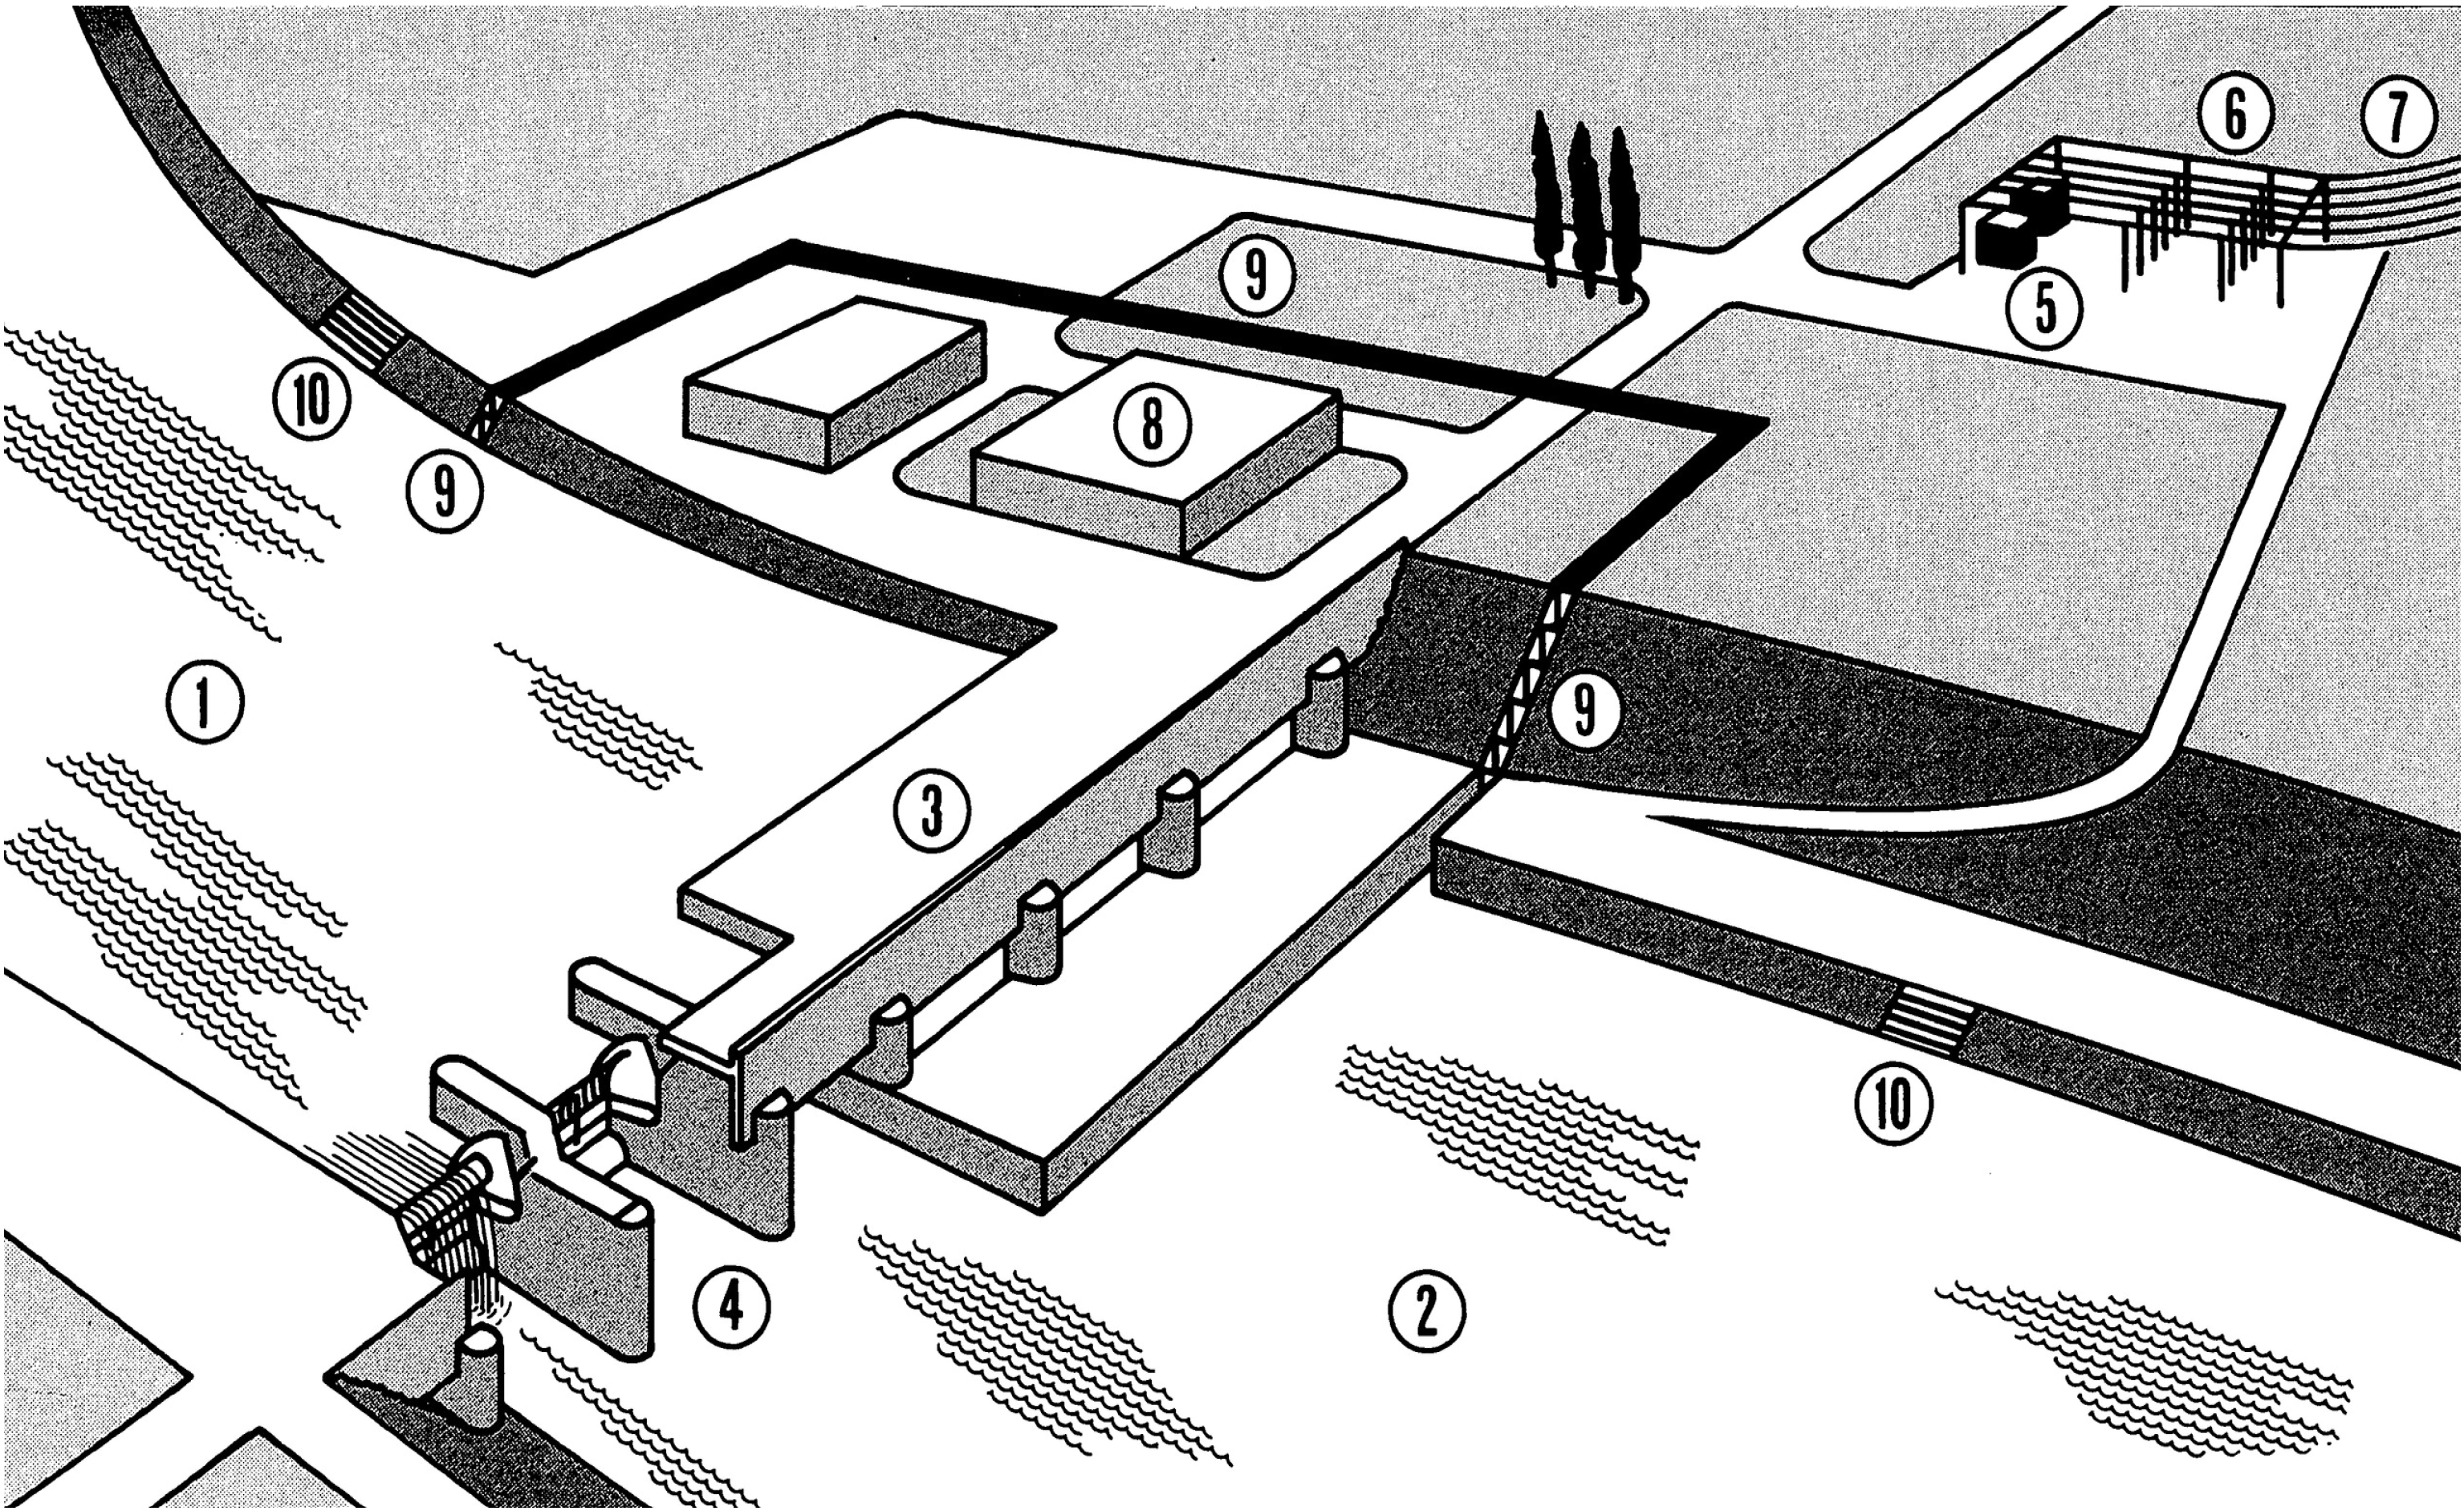
\includegraphics[width=0.95\columnwidth, align=c]{images/Laufwasserkraftwerke.png}
\end{center}

\begin{minipage}[c]{0.38\columnwidth}
    \begin{tabular}{c l}
        1 & Oberwasser \\ 
        2 & Unterwasser \\ 
        3 & Maschinenhaus \\
        4 & Stauwehr \\
        5 & Transformatoren \\
    \end{tabular}
\end{minipage}
\hfill
\begin{minipage}[c]{0.58\columnwidth}
    \begin{tabular}{c l}
        6 & Schaltanlage \\
        7 & Leitungen \\
        8 & Betriebsgebäude \\
        9 & Fischtreppe \\
        10 & Einrichtung für den Schiffstransport \\
    \end{tabular}
\end{minipage}

\newcolumn

\subsection{LWK mit Kaplanturbinen}

\begin{itemize}
    \item Turbine Vertikal verbaut
\end{itemize}

\begin{center}
    \includegraphics[width=0.95\columnwidth, align=c]{images/Laufwasserkraftwerke_Kaplanturbine_Vertikal.png}
\end{center}

\begin{minipage}[t]{0.38\columnwidth}
    \begin{tabular}{c l}
        1 & Oberwasser \\
        2 & Unterwasser \\
        3 & Rechen \\
        4 & Spirale \\
        5 & Stützschaufeln \\
        6 & Leitschaufeln \\
        7 & Laufrad \\
        8 & Laufradschaufeln \\
        9 & Saugrohr \\
    \end{tabular}
\end{minipage}
\hfill
\begin{minipage}[t]{0.58\columnwidth}
    \begin{tabular}{c l}
        10 & Generator \\
        11 & Maschinenhaus \\
        12 & Rechenreinigungsmaschine \\
        13 & Geschwemmselrinne \\
        14 & Zangengreifer \\
        15 & Dammbalken \\
        16 & Nuten für Dammbalken \\
        17 & Dammbalkenkran \\
           &  \\
    \end{tabular}
\end{minipage}



\subsection{LWK mit Rohrturbinen}

\begin{itemize}
    \item Turbine Horizontal verbaut
    \item bis 25m Fallhöhe
\end{itemize}

\begin{center}
    \includegraphics[width=0.95\columnwidth, align=c]{images/Laufwasserkraftwerke_Kaplanturbine_Horizontal.png}
\end{center}

\begin{minipage}[t]{0.38\columnwidth}
    \begin{tabular}{c l}
        1 & Oberwasser \\
        2 & Unterwasser \\
        3 & Rechen \\
        4 & Leitschaufeln \\
        5 & Laufrad \\
        6 & Laufradschaufeln \\
        7 & Turbinenwelle \\
        8 & Generator \\
        9 & Gehäuse \\
    \end{tabular}
\end{minipage}
\hfill
\begin{minipage}[t]{0.58\columnwidth}
    \begin{tabular}{c l}
        10 & Sockel \\
        11 & Einstiegsschächte \\
        12 & Maschinenhalle \\
        13 & Rechenreinigungsmaschine \\
        14 & Geschwemmselrinne \\
        15 & Zangengreifer \\
        16 & Dammbalken \\
        17 & Nuten für die Dammbalken \\
        18 & Dammbalkenkran \\
    \end{tabular}
\end{minipage}
\subsection{Wasserwirbelkraftwerk}

\begin{minipage}[c]{0.58\columnwidth}
    \begin{itemize}
    \item Für Kleinwasserkraft
    \item Geringe Fallhöhen und Durchfluss möglich:\\
    $h \geqq 0.5\text{m}$ und $Q \geqq 0.5 \frac{\text{m}^3}{\text{s}}$
    \item Geringerer Wirkungsgrad
    \item Besser Fischgängig
\end{itemize}
\end{minipage}
\hfill
\begin{minipage}[c]{0.38\columnwidth}
    \includegraphics[width=0.65\columnwidth, align=c]{images/Wasserwirbelkraftwerk.jpg}
\end{minipage}

\newcolumn
\subsection{LWK mit Strafloturbinen}

\begin{itemize}
    \item Weiterentwicklung der Rohrturbine
    \item Rotor Turbine und Generator bilden Einheit
\end{itemize}

\begin{center}
    \includegraphics[width=0.95\columnwidth, align=c]{images/Laufwasserkraftwerke_mit_Strafloturbinen.png}
\end{center}

\begin{minipage}[t]{0.38\columnwidth}
    \begin{tabular}{c l}
        1 & Laufradnabe \\
        2 & Propellerblatt \\
        3 & Rotorring \\
        4 & Entlastungsring \\
        5 & Turbinengehäuse \\
        6 & Leitschaufel \\
        7 & Leitradverstellring \\
    \end{tabular}
\end{minipage}
\hfill
\begin{minipage}[t]{0.58\columnwidth}
    \begin{tabular}{c l}
        8 & Rohrleitung \\
        9 & Generator \\
        10 & Stator \\
        11 & Rotor \\
        12 & Ringdichtungs-Leckwasser-Kollektor \\
        13 & Leckwasserableitung \\
        14 & Kühler \\
    \end{tabular}
\end{minipage}

\subsection{Mitteldruckanlagen}

\begin{itemize}
    \item bis circa 50m Fallhöhe
    \item (<= 5 bar Druck)
\end{itemize}

\subsection{Pumpspeicherkraftwerke (PSW)}

\begin{itemize}
    \item Pumpspeicherkraftwerk mit konventionellem Maschinensatz (Dreimaschinensatz)
    \item Wirkungsgrad der PSW: 65 – 80\%
\end{itemize}

\begin{center}
    \includegraphics[width=0.75\columnwidth, align=c]{images/Pumpspeicherkraftwerke.png}
\end{center}

\begin{minipage}[t]{0.48\columnwidth}
    \begin{tabular}{c l}
        1 & Unteres Becken \\
        2 & Oberes Becken \\
        3 & Energieableitung, Stromleitung \\
        4 & Motorgenerator \\
    \end{tabular}
\end{minipage}
\hfill
\begin{minipage}[t]{0.48\columnwidth}
    \begin{tabular}{c l}
        5 & Kupplung \\
        6 & Kugelschieber \\
        7 & Pumpe \\
        8 & Turbine \\
    \end{tabular}
\end{minipage}

\subsubsection{Maschinensatz}
\begin{tabular}{c c}
    Zweimaschinensatz:  & Motor/Generator und Pumpturbine \\
    Dreimaschinenesatz: & Motor/Generator, Turbine und Pumpe
\end{tabular}
\newcolumn

\subsection{Hochdruck- (Speicher-) Anlagen}

\begin{itemize}
    \item ab circa 50m Fallhöhe
    \item (> 5 bar Druck, bis weit über 100 bar möglich)
\end{itemize}

\begin{center}
    \includegraphics[width=0.85\columnwidth, align=c]{images/Hochdruckspeicheranlagen.png}
\end{center}

\begin{minipage}[t]{0.48\columnwidth}
    \begin{tabular}{c l}
        1 & Stausee \\
        2 & Wasserfassung \\
        3 & Freispiegelstollen (keine Druckleitung) \\
        4 & Staumauer \\
        5 & Grundablass (für kontrollierten Ablauf) \\
        6 & Hochwasserentlastung (= Überlauf) \\
        7 & Einlauf \\
        8 & Drosselklappe\\ & (Wasserfluss Druckstollen steuern) \\
        9 & Druckstollen \\
    \end{tabular}
\end{minipage}
\hfill
\begin{minipage}[t]{0.48\columnwidth}
    \begin{tabular}{c l}
        10 & Wasserschloss (Druckausgleich\\ & Änderung Wasserdurchfluss) \\
        11 & Druckschacht \\
        12 & Zentrale \\
        13 & Turbine \\
        14 & Kugelschieber \\
        15 & Generator \\
        16 & Energieableitung, Transformatoren \\
        17 & Schaltanlage \\
        18 & Unterwasserstollen \\
    \end{tabular}
\end{minipage}
\subsubsection{Stollen und Schächte}

\begin{tabular}{l l}
     Freispiegelstollen: &  flach, nicht voll gefüllt, Umgebungsdruck\\
     Druckstollen (Betonverkl.): & flach, voll gefüllt, Druck $>$ Umgebungsdr. , $v < 5\,\mathrm{m/s}$ \\
     Druckschacht (Stahlpanzerung): & steil, voll gefüllt, Druck $\gg$ Umgebungdr. , $v < 9\,\mathrm{m/s}$ 
\end{tabular}



\subsection{Wasserschloss}
Das Wasserschloss ist ein nach oben offenes Gefäss.
Im Druckstollen sind grosse Wassermassen vorhanden. Diese Wassermassen müssen:

\begin{itemize}
    \item beim Anfahren der Maschinengruppen beschleunigt,
    \item beim Abstellen gebremst werden.
\end{itemize}
Das Wasserschloss dient als Puffer

\begin{center}
    \includegraphics[width=0.75\columnwidth, align=c]{images/Wasserschloss.jpg}
\end{center}


$
\boxed{V_{\mathrm{St}} = l_{\mathrm{St}} \cdot A_{\mathrm{St}}} 
\quad
\boxed{m_{\mathrm{wSt}} = \rho_{\mathrm{w}} \cdot V_{\mathrm{St}}}
\quad
\boxed{v_{\mathrm{St}}= \frac{Q}{A_{\mathrm{St}}}}\\
\quad
\boxed{V_{\mathrm{s}} = l_{\mathrm{s}} \cdot A_{\mathrm{s}}^2}
\quad
\boxed{m_{\mathrm{ws}} = \rho_{\mathrm{w}} \cdot V_{\mathrm{St}}}
\quad
\boxed{v_{\mathrm{s}}= \frac{Q}{A_{\mathrm{s}}}}\\
\quad
\boxed{E_{\mathrm{kSt}} = \frac{m_{\mathrm{wSt}} \cdot V_{\mathrm{St}}}{2}}
\quad
\boxed{E_{\mathrm{ks}} = \frac{m_{\mathrm{ws}} \cdot V_{\mathrm{s}}}{2}}
\quad
\boxed{E_{\mathrm{ktot}} = E_{\mathrm{kSt}}+E_{\mathrm{ks}}}\\
\quad
\boxed{E_{\mathrm{pot}} = E_{\mathrm{ktot}}}
\quad
\quad
\boxed{h_{\mathrm{ws}} = \sqrt{\frac{E_{\mathrm{pot}} \cdot 2}{\rho_{\mathrm{w}} \cdot A_{\mathrm{ws}} \cdot g}}}
$
\vspace{0.15cm}

\renewcommand{\arraystretch}{1.2}
\begin{tabular}{@{} l p{7cm} l @{}}    
    $[l_{\mathrm{St}}]$     & Stollenlänge \dotfill                                         & $\mathrm{m}$ \\
    $[A_{\mathrm{St}}]$     & Stollenfläche \dotfill                                        & $\mathrm{m^2}$ \\
    $[V_{\mathrm{St}}]$     & Stollenvolumen \dotfill                                       & $\mathrm{m^3}$ \\
    $[m_{\mathrm{wSt}}]$    & Wassermasse im Stollen \dotfill                               & $\mathrm{kg}$ \\
    $[v_{\mathrm{wSt}}]$    & Fliessgeschwindigkeit im Stollen \dotfill                     & $\mathrm{m/s}$ \\
    $[\rho_{\mathrm{w}}]$   & Dichte des Wassers ($1000\, \mathrm{kg/m^3}$) \dotfill        & $\mathrm{kg/m^3}$ \\
    $[Q]$                   & Druchfluss \dotfill                                           &$\mathrm{m^3/s}$\\
    $[l_{\mathrm{s}}]$      & Schachtlänge \dotfill                                         & $\mathrm{m}$ \\
    $[A_{\mathrm{s}}]$      & Schachtfläche \dotfill                                        & $\mathrm{m^2}$ \\
    $[V_{\mathrm{s}}]$      & Schachtvolumen \dotfill                                       & $\mathrm{m^3}$ \\
    $[m_{\mathrm{ws}}]$     & Wassermasse im Schacht \dotfill                               & $\mathrm{kg}$ \\
    $[v_{\mathrm{s}}]$      & Fliessgeschwindigkeit im Schacht\dotfill                      & $\mathrm{m/s}$ \\
    $[E_{\mathrm{kSt}}]$    & Kinetische Energie im Stollen                                 & $\mathrm{J}$\\
    $[E_{\mathrm{ks}}]$     & Kinetische Energie im Schacht                                 & $\mathrm{J}$\\
    $[E_{\mathrm{pot}}]$    & Potentielle Energie                                           & $\mathrm{J}$\\
    $[A_{\mathrm{ws}}]$     & Wasserschlossfläche \dotfill                                  & $\mathrm{m^2}$ \\
    $[h_{\mathrm{ws}}]$     & Höhe des Wasserspiegels im Wasserschloss \dotfill             & $\mathrm{m^2}$ \\
    $[g]$                   & Fallbeschleunigung $(9.81\, \mathrm{m/s^2})$ \dotfill         & $\mathrm{m^2}$ \\
    
    
    
    

    
    
\end{tabular}

\subsection{Gezeitenkraftwerke}

\begin{itemize}
    \item Nutzung des Tidenhubs
    \item Früher meist mit Staudammbauweise (hohe Umwelteinwirkungen)
    \item Heute meist Meeresströmungs-Kraftwerk
    \item Grösste Europäische Anlage in Frankreich (240 MW)
\end{itemize}


\subsection{Wellenkraftwerk}

\subsubsection{Wellenkraftwerk mit Pneumatischer Kammer}
\includegraphics[width=0.55\columnwidth, align=c]{images/Wellenkraft mit Pneumatischer Kammer.png}


\subsubsection{Wellenkraftwerk mit Rampe}
\includegraphics[width=0.55\columnwidth, align=c]{images/Wellenkraft mit Rampe.png}


        \newpage
\section{Kenngrössen Turbinen}

\subsection{Hydraulische Leistung}

$\boxed{P_{\text{hyd}} = \rho \cdot Q \cdot g \cdot H_n}$

\vspace{0.15cm}

\renewcommand{\arraystretch}{1.2} % Erhöht Zeilenhöhe für bessere Lesbarkeit
\begin{tabular}{@{} l p {7cm} l @{}}
    $[P_{\text{hyd}}]$  & Hydraulische Leistung \dotfill & $\mathrm{W}$ \\
    $[Q]$               & Nutzwassermenge \dotfill & $\mathrm{\frac{m^3}{s}}$ \\
    $[H_n]$             & Nettofallhöhe \dotfill & $\mathrm{m}$ \\
    $[\rho]$            & Dichte des Wassers ($\rho = 1000$) \dotfill & $\mathrm{\frac{kg}{m^3}}$ \\
    $[g]$               & Erdbeschleunigung ($g = 9.81$) \dotfill & $\mathrm{\frac{m}{s^2}}$ \\
\end{tabular}



\subsection{Mechanische Leistung an der Turbinenwelle}

$\boxed{P_{\text{mech}} = \omega \cdot M} \quad \boxed{P_{\text{mech}} = \eta_t \cdot P_{\text{hyd}}}$

\vspace{0.15cm}

\renewcommand{\arraystretch}{1.2} % Erhöht Zeilenhöhe für bessere Lesbarkeit
\begin{tabular}{@{} l p {6cm} l @{}}
    $[P_{\text{mech}}]$  & Mechanische Leistung   \dotfill & $\mathrm{W}$ \\
    $[\omega]$           & Winkelgeschwindigkeit \dotfill & $\mathrm{\frac{rad}{s}}$ \\
    $[\eta_t]$           & Wirkungsgrad Turbine \dotfill & $-$ \\
    $[M]$                & Drehmoment            \dotfill & $\mathrm{Nm}$ \\
\end{tabular}



\subsection{Winkelgeschwindigkeit}

$\boxed{\omega = 2 \cdot \pi \cdot n}$

\vspace{0.15cm}

\renewcommand{\arraystretch}{1.2} % Erhöht Zeilenhöhe für bessere Lesbarkeit
\begin{tabular}{@{} l p {6cm} l @{}}
    $[\omega]$  & Winkelgeschwindigkeit \dotfill & $\mathrm{\frac{rad}{s}}$ \\
    $[n]$       & Drehzahl              \dotfill & $\mathrm{\frac{1}{s}}$ \\
\end{tabular}



\subsection{Betriebszustände der Maschinengruppe}
\textbf{(Maschinengruppe = Turbine/Pumpe + Generator/Motor)}

\begin{itemize}
    \item Inselbetrieb
    \item Parallelbetrieb, Verbundbetrieb
    \item Instationäre Vorgänge
    \begin{itemize}
        \item Anfahren und Abstellen
        \item Lastabwurf $\Rightarrow$ Überdrehzahl
    \end{itemize}
\end{itemize}

\textbf{Durchgangsdrehzahl $n_D$} (auch Schleuderdrehzahl genannt)

$\Rightarrow$ höchste erreichbare Drehzahl ohne Last (z.B. bei Versagen des Generators)

Die Durchgangsdrehzahl ist eine Bemessungsgröße. 

Die Maschinengruppe darf bei der Durchgangsdrehzahl keinen Schaden erleiden.

\subsection{Spezifische Drehzahl $n_q$}

\noindent
$
\boxed{
n_q = n \cdot \frac{\sqrt{Q}}{H_n^{3/4}}
}
$

\vspace{0.15cm}

\renewcommand{\arraystretch}{1.2}
\begin{tabular}{@{} l p{6cm} l @{}}
    $[n_q]$          & Spezifische Drehzahl \dotfill                               & $\text{U/min}$ \\
    $[n]$            & Drehzahl der Turbine \dotfill                               & $\text{U/min}$ \\
    $[Q]$            & Nutzwassermenge \dotfill                                    & $\frac{\text{m}^3}{\text{s}}$ \\
    $[H_n]$          & Nettofallhöhe \dotfill                                      & $\text{m}$ \\
\end{tabular}

\vspace{0.15cm}

$n_q$ ist die Drehzahl einer Turbine in \(\mathrm{U/min}\), welche bei einem Gefälle von \(1 \,\mathrm{m}\) einen Volumenstrom von \(1 \,\mathrm{m}^3/\mathrm{s}\) aufweist (Ähnlichkeitsgesetz).




\myul{\textbf{Typische $n_q$}}

\vspace{0.15cm}

\textbf{Peltonturbinen} \hspace{1cm} $<$ 20 U/min 

\vspace{0.15cm}

\textbf{Francisturbinen} \hspace{1cm} ca. 20 bis ca. 100 U/min 

\vspace{0.15cm}

\textbf{Kaplanturbinen} \hspace{1cm} $>$ 100 U/min



\newcolumn
\section{Turbinen}

\subsection{Peltonturbine}

\begin{minipage}[c]{0.48\columnwidth}
    \includegraphics[width=0.98\columnwidth, align=c]{images/Pelton_Turbine_1.png}    
\end{minipage}
\hfill
\begin{minipage}[c]{0.48\columnwidth}
    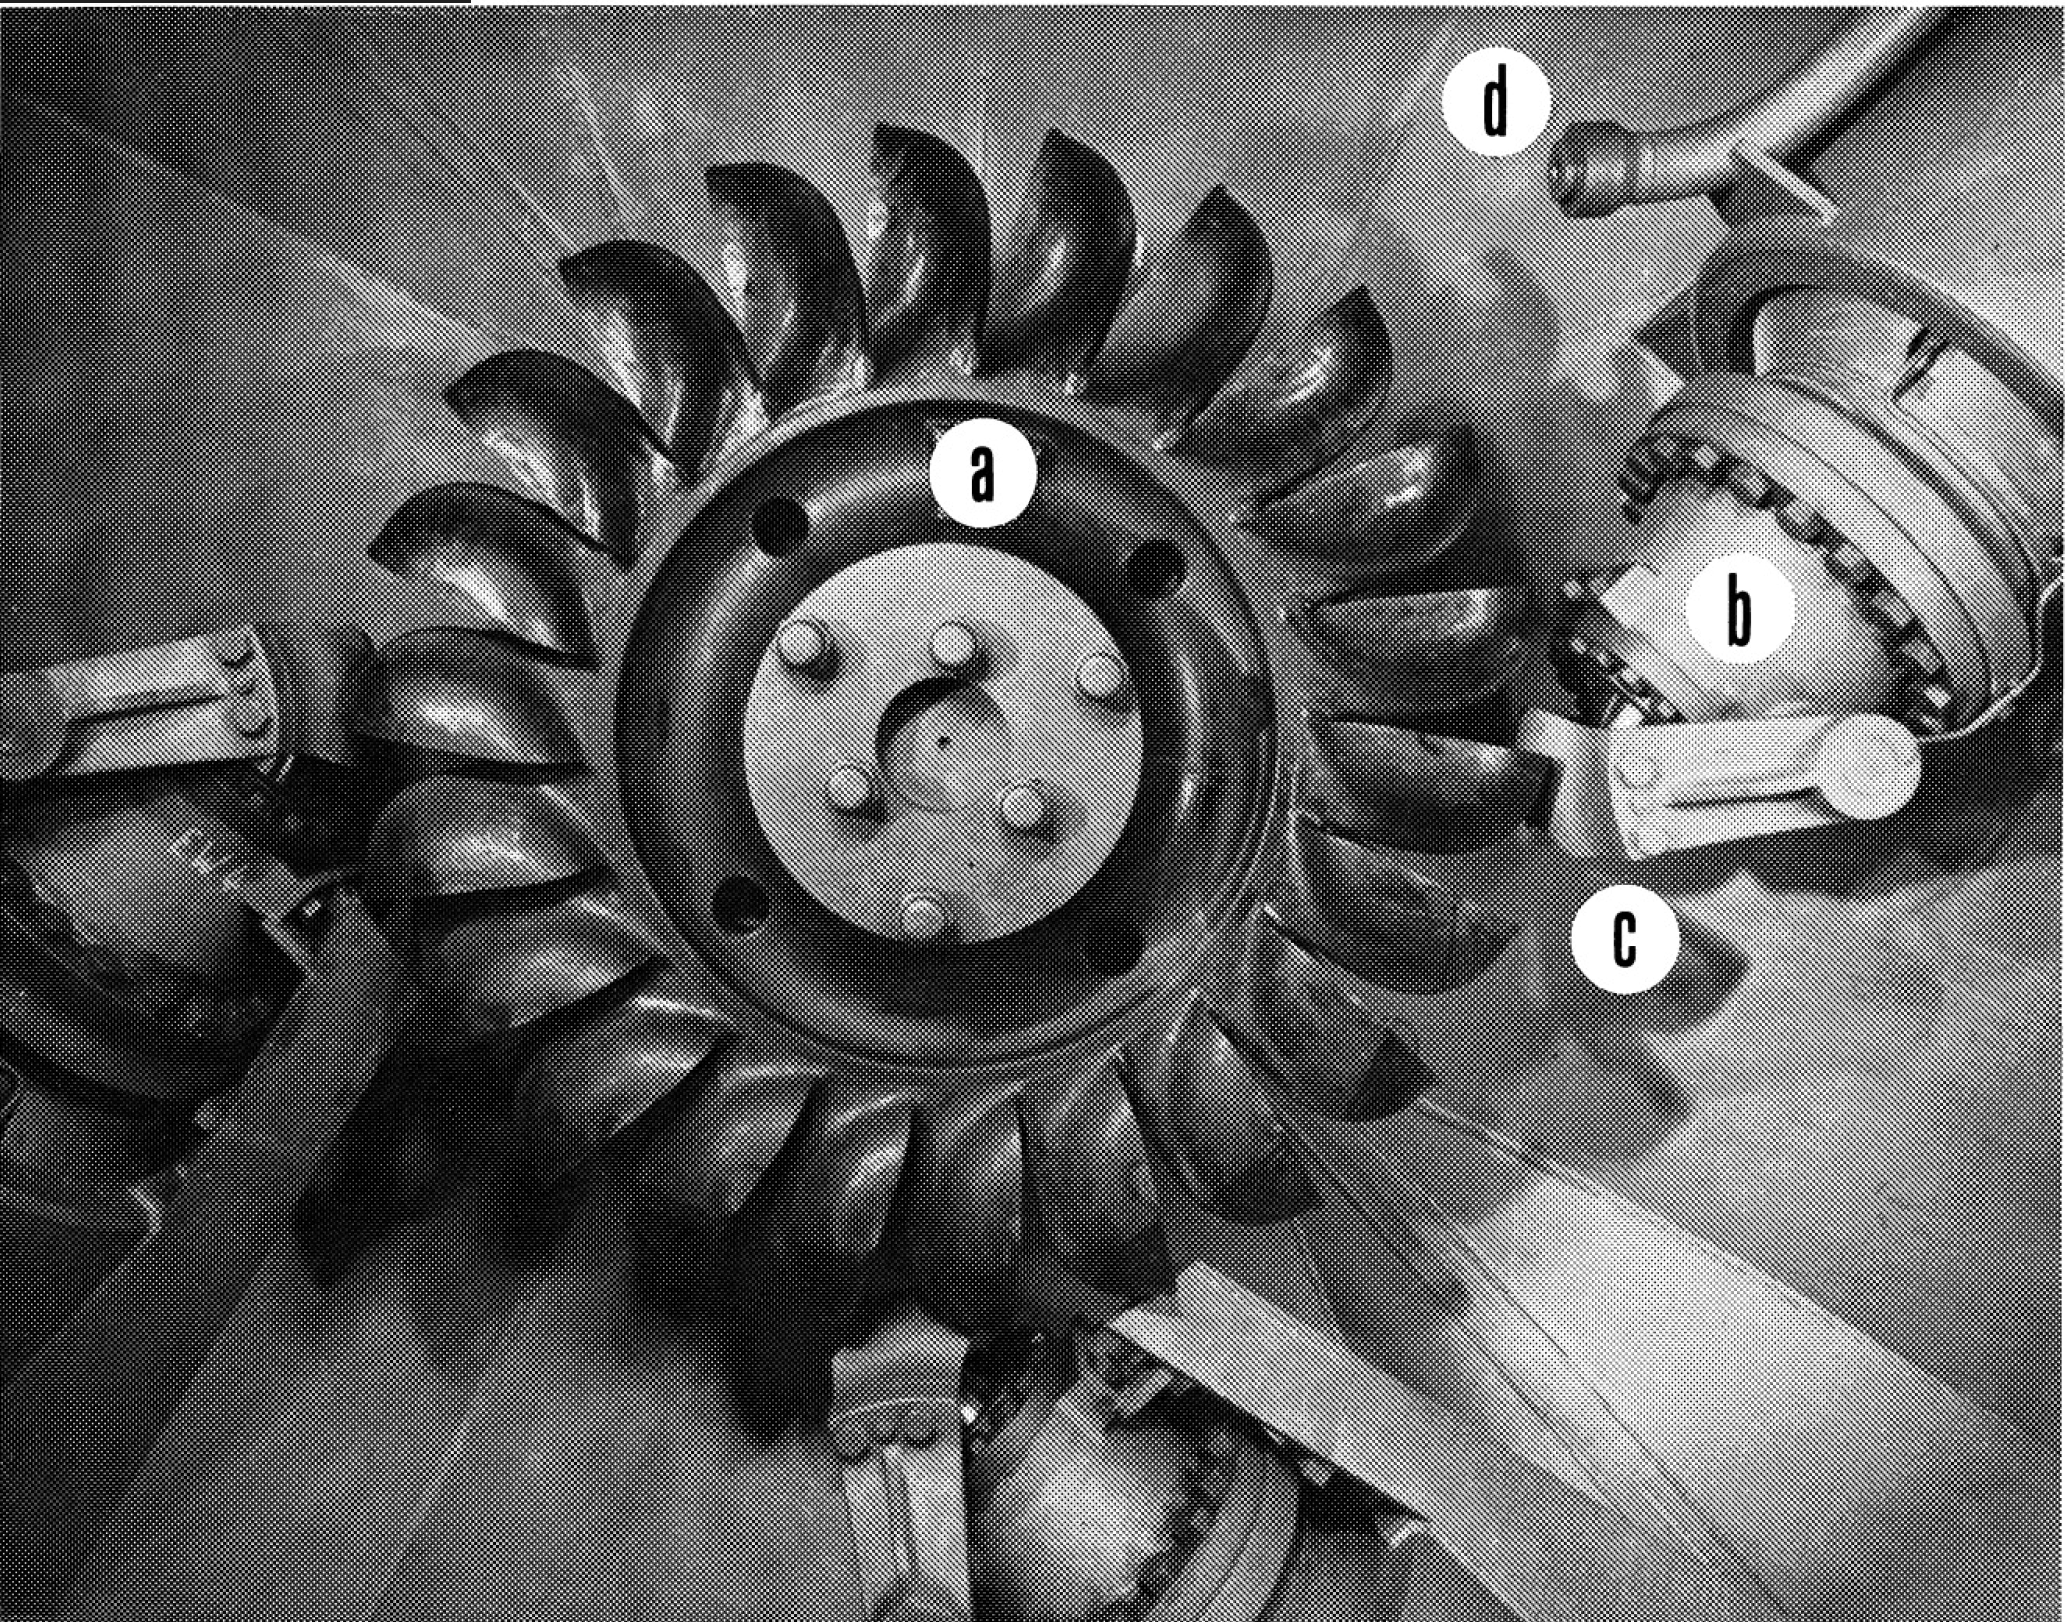
\includegraphics[width=0.98\columnwidth, align=c]{images/Pelton_Turbine_2.png}   
\end{minipage}

\begin{tabular}{c l}
    a & Peltonrad \\
    b & Düse \\
    c & Strahlablenker \\
    d & Bremsdüse \\
\end{tabular}

\vspace{0.15cm}

\begin{minipage}[c]{0.48\columnwidth}
    Düse offen    
\end{minipage}
\hfill
\begin{minipage}[c]{0.48\columnwidth}
    Düse geschlossen   
\end{minipage}

\begin{minipage}[c]{0.48\columnwidth}
    \includegraphics[width=0.98\columnwidth, align=c]{images/Pelton_Turbine_Düse_offen.png}    
\end{minipage}
\hfill
\begin{minipage}[c]{0.48\columnwidth}
    \includegraphics[width=0.98\columnwidth, align=c]{images/Pelton_Turbine_Düse_geschlossen.png}   
\end{minipage}

\begin{tabular}{c l}
        1 & Düsennadel \\
        2 & Kolben \\
        3 & Öl zum öffnen \\
        4 & Öl zum Schliessen \\
        5 & Rückmeldung
\end{tabular}

\subsubsection{Eingenschaften und Merkmale}
\begin{itemize}
    \item Guter Wirkungsgrad über einen großen Einsatzbereich von 10 bis 100\% der max. Leistung
    \item Unkritische Maschine
    \item Der sogenannte Gletscherschliff muss beachtet werden (Erosion am Laufrad)
    \item Verschraubung Rad- / Generatorflansch (Kupplung) mit z.B. mechanisch vorgespannten Dehnschrauben
    \item Trockenenlegung der Kupplung
    \item Wirkungsgradverbesserungen oft möglich
    \item Rissen im Bereich der Becherwurzel (hochbelastete Zone) gilt ein spezielles Augenmerk
\end{itemize}



\subsection{Reaktionsturbinen}

\begin{itemize}
    \item Francisturbinen
    \item Kaplanturbinen
    \item Rohrturbinen
    \item Kreiselpumpen als Turbinen
\end{itemize}



\subsubsection{Funktionsprinzip}

\textbf{Turbinenspirale (TS)}: exzentrisch zur Turbinenachse angeordneter Zulaufkanal, der die durch eine \textbf{Turbinenspirale} erzeugte Drallströmung (\textbf{DS}) veranschaulicht (<<Badewannenablass>>)

\textbf{Laufrad (LR)}: Schaufelrad, welches das in der \textbf{Drallströmung} DS platzierte Laufrad der Turbine darstellt

\includegraphics[width=0.58\columnwidth, align=c]{images/Laufradturbinen.png}   



\subsubsection{Kavitation}

\includegraphics[width=0.98\columnwidth, align=c]{images/Kavitation.png}   

\renewcommand{\arraystretch}{1.2} % Erhöht Zeilenhöhe für bessere Lesbarkeit
\begin{tabular}{@{} l p {7cm} l @{}}
    $[w]$   & Rel. Geschw. des Wassers bez. der drehenden Schaufel  \dotfill & $\mathrm{\frac{m}{s}}$ \\
    $[u]$   & Umfanggeschwindigkeit der Schaufel                    \dotfill & $\mathrm{\frac{m}{s}}$ \\
\end{tabular}

\vspace{0.15cm}

\begin{tabular}{ll}
\hline
\textbf{Turbinentyp} & \({n_D}/{n_N}\) \\
\hline
Francis, \(n_q = 40 \ldots 80\) U/min & \(1.7 \ldots 2.0\) \\
Francis, \(n_q = 80 \ldots 120\) U/min & \(2.0 \ldots 2.2\) \\
Propeller, feste Lauf- und Leitschaufeln & \(1.8 \ldots 2.2\) \\
Kaplan, verstellbare Laufschaufeln, feste Leitschaufeln & \(2.4 \ldots 2.8\) \\
Kaplan, verstellbare Lauf- und Leitschaufeln & \(2.4 \ldots 3.2\) \\
Pumpen im Turbinenbetrieb, \(n_q = 30 \ldots 100\) U/min & \(1.4 \ldots 1.8\) \\
\hline
\end{tabular}

\vspace{0.15cm}

Je grösser \({n_D}/{n_N}\) desto stärker muss die Turbine dimensioniert werden

\vspace{0.15cm}

\textbf{Verhältnis der Volumenströme bei Durchgangs- bzw. Nenndrehzahl:}

$
\begin{aligned}
   n_q < 100 \ \mathrm{U/min:} & \quad Q_D < Q_N \\
    n_q = 100 \ \mathrm{U/min:} & \quad Q_D = Q_N \\
    n_q > 100 \ \mathrm{U/min:} & \quad Q_D > Q_N 
\end{aligned}
$

\vspace{0.15cm}

\begin{itemize}
    \item \textbf{Durchgangsdrehzahl} \(n_D\)
    \item \textbf{Nenndrehzahl} \(n_N\)
    \item \textbf{Spezifische Drehzahl} \(n_q\)
\end{itemize}

\vspace{0.15cm}

\renewcommand{\arraystretch}{1.2} % Erhöht Zeilenhöhe für bessere Lesbarkeit
\begin{tabular}{@{} l p {7cm} l @{}}
    $[n_D]$   & Drehzahl bei Lastabwurf (plötzlicher Generatorverlust)  \dotfill & $\mathrm{\frac{U}{min}}$ \\
    $[n_N]$   & Tatsächliche Drehzahl im Normalbetrieb                    \dotfill & $\mathrm{\frac{U}{min}}$ \\
    $[n_q]$   & Drehzahl einer skalierten Maschine  \(\left(H = 1\,\mathrm{m},\, Q = 1\,\mathrm{m}^3/\mathrm{s}\right)\)                  \dotfill & $\mathrm{\frac{U}{min}}$ \\
\end{tabular}



\subsection{Francisturbinen}

\begin{minipage}[c]{0.48\columnwidth}
    \includegraphics[width=0.98\columnwidth, align=c]{images/Francis_Turbine.png}    
\end{minipage}
\hfill
\begin{minipage}[t]{0.48\columnwidth}
    \begin{tabular}{c l}
        1 & Einlaufspirale \\
        2 & Leitschaufeln \\
        3 & Leitschaufelnachse \\
        4 & Laufrad \\
        5 & Turbinenwelle
\end{tabular}  
\end{minipage}



\subsection{Kaplanturbinen}

\begin{minipage}[c]{0.48\columnwidth}
    \includegraphics[width=0.98\columnwidth, align=c]{images/Kaplan_Turbine.png}    
\end{minipage}
\hfill
\begin{minipage}[t]{0.48\columnwidth}
    \begin{tabular}{c l}
        1 & Einlaufspirale \\
        2 & Stützschaufeln \\
        3 & Leitschaufeln \\
        4 & Kaplan-Rad \\
\end{tabular}  
\end{minipage}



\subsection{Rohrturbinen (= horizontale Kaplanturbinen)}

\begin{minipage}[c]{0.48\columnwidth}
    \includegraphics[width=0.98\columnwidth, align=c]{images/Rohr_Turbinen.png}    
\end{minipage}
\hfill
\begin{minipage}[t]{0.48\columnwidth}
    \begin{tabular}{c l}
        1 & Schaufelrad \\
        2 & Leitschaufeln \\
        3 & Zustiegsschächte \\
        4 & Demontageschacht \\
        5 & Sockel \\
        6 & Generator \\
\end{tabular}  
\end{minipage}



\subsection{Strafloturbinen}
\begin{minipage}[c]{0.48\columnwidth}
    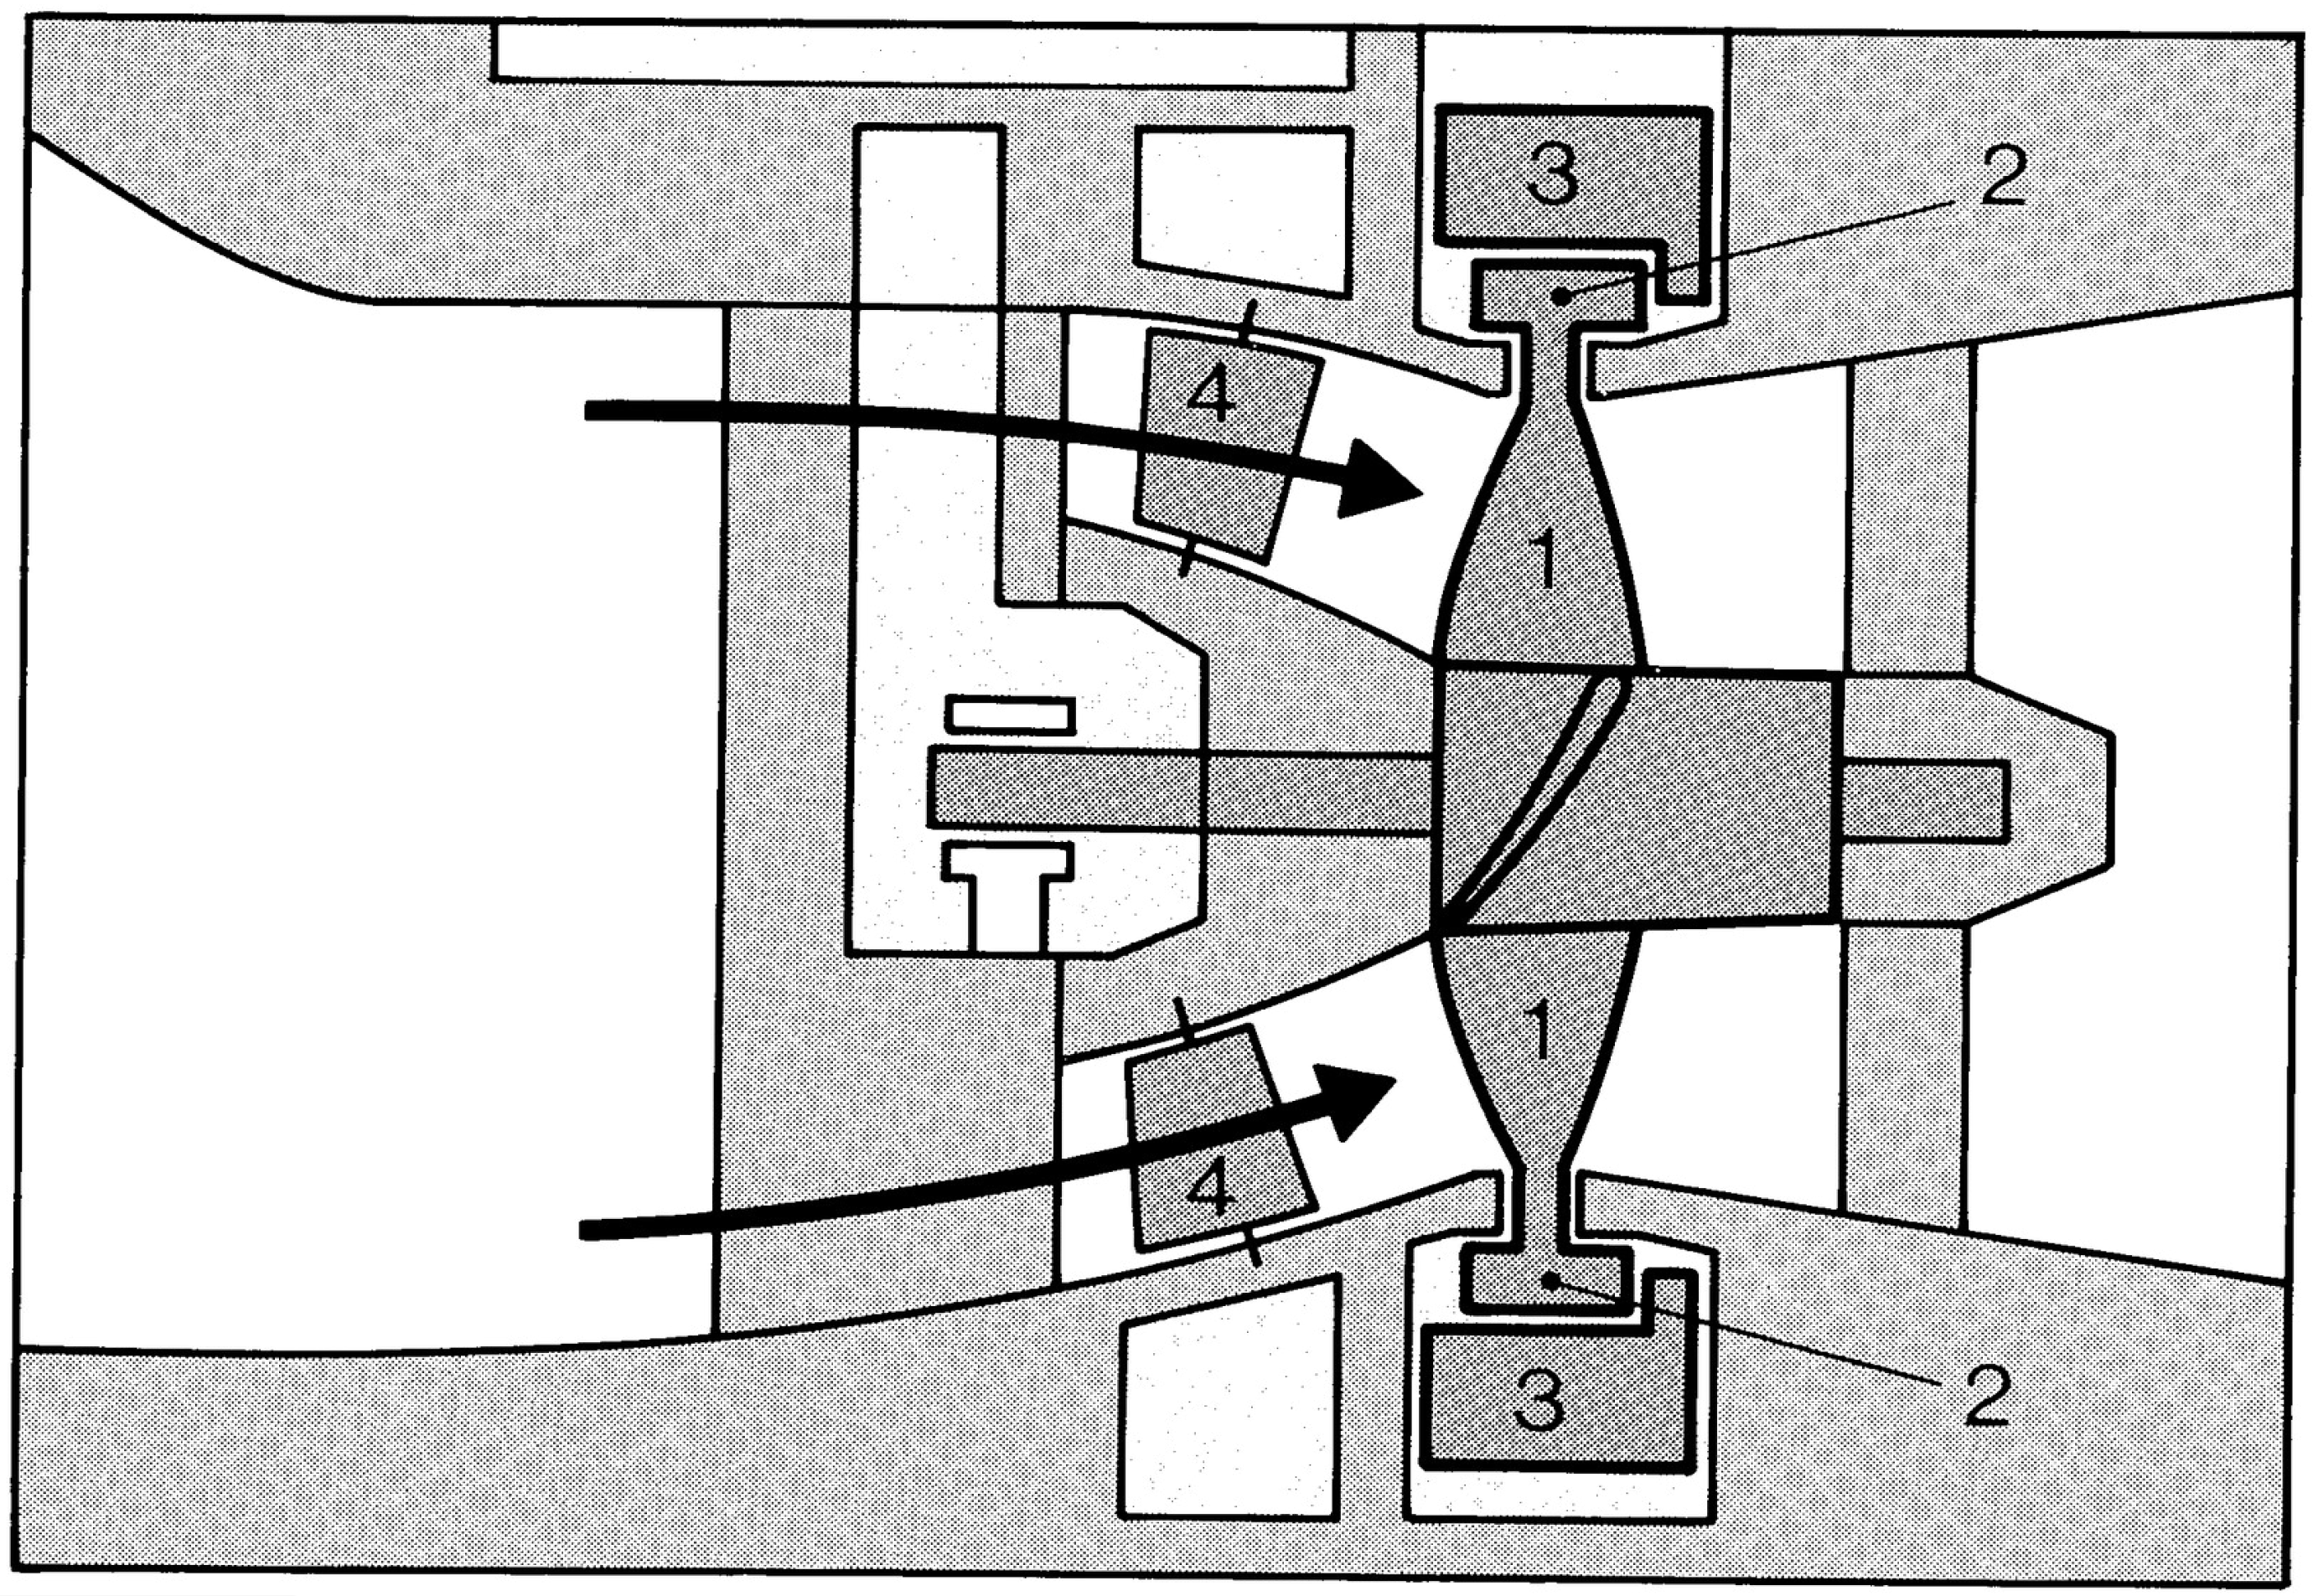
\includegraphics[width=0.98\columnwidth, align=c]{images/Straflo_Turbine.png}    
\end{minipage}
\hfill
\begin{minipage}[t]{0.48\columnwidth}
    \begin{tabular}{c l}
        1 & Laufradschaufeln \\
        2 & Rotor, Pole des Generators \\
        3 & Stator \\
        4 & Leitschaufeln \\
\end{tabular}  
\end{minipage}

\subsection{Speicherpumpen und Pumpturbinen}
\includegraphics[width=0.98\columnwidth, align=c]{images/Speicherpumpen und Pumpturbinen.png}   

\subsubsection{Dreimaschinensatz}

Besteht aus: Generator/Motor, Francisturbine und Speicherpumpe

\vspace{0.15cm}

    \textcolor{red}{\textbf{Nachteile}} 
    \begin{itemize}
        \item Zwei hydraulische Maschinen sowie eine größere Anzahl Abschlussorgane sind nötig.
    \end{itemize}
    \textcolor{green}{\textbf{Vorteil}}
    \begin{itemize}
        \item Unabhängige Optimierung der Turbine und der Pumpe ist möglich.
    \end{itemize}




\subsection{Wahl des Generators}

Der Generator muss synchron mit dem Netz drehen. Daher muss die definitive Drehzahl der in der Nähe liegenden Synchrondrehzahl entsprechen.

\vspace{0.15cm}

$
\boxed{n = 60 \cdot \frac{f}{p} } \quad \boxed{n = \frac{3000}{p}}
$

\vspace{0.15cm}

\renewcommand{\arraystretch}{1.2}
\begin{tabular}{@{} l p{6cm} l @{}}
    $[n]$           & Drehzahl des Generators \dotfill                         & $\text{U/min}$ \\
    $[f]$           & Frequenz, meist 50 Hz \dotfill                            & $\text{Hz} = \frac{1}{\text{s}}$ \\
    $[p]$           & Polpaarzahl \dotfill                                      & (1, 2, 3, \dots) \\
\end{tabular}


\subsection{Kochrezept zur Grob-Auslegung von Pumpen und Turbinen}

\begin{enumerate}
    \item Bestimmung der \textbf{Netto-Fallhöhe} \( H_n \)
    \item Auswahl \textbf{Gesamtdurchfluss} \( Q \), abhängig von Zufluss, Rückhaltemöglichkeit, Einsatztyp (z.B. Spitzenlast)
    \item Bestimmung der \textbf{hydraulischen Leistung}:
    \[
    P_\mathrm{hyd} = \rho \cdot Q \cdot g \cdot H_n
    \]
    \item Auswahl \textbf{Turbinentyp}, \textbf{Turbinen-Durchfluss} \( Q \) und \textbf{spezifische Drehzahl} \( n_q \) aus Diagrammen\\
    (ggf. Aufteilung \( Q \) auf mehrere Turbinen / Pumpen)
    \item Bestimmung der \textbf{Turbinen-Drehzahl}:
    \[
    n = n_q \cdot \frac{H_n^{3/4}}{Q^{1/2}}
    \]
    \item Bestimmung der \textbf{Polpaarzahl}:
    \[
    p = \frac{3000}{n}
    \]
    (auf ganze Zahl runden und prüfen, ob \( n_q \) nach Rundung noch im möglichen Bereich liegt)
    \item Weitere Bedingungen zur \textbf{Feinauslegung}:
    \begin{itemize}
        \item Teillastverhalten, Wirkungsgrad, Betriebsbereiche
        \item Räumliche Bedingungen, Simulationen, Experimente
        \item \(\ldots\)
        \item Lösung ist ein Abwägen und iterativer Prozess
    \end{itemize}
\end{enumerate}



















        \section{Thermische Kraftwerke/ Dampfkraftwerke}
Gegen 90\% der weltweiten Bereitstellung
elektrischer Energie erfolgt in «Thermischen Kraftwerken».\\
Kraftwerksarten:
\begin{itemize}
    \item Thermische Kraftwerke auf fossiler Basis
(Dampf-, Gasturbinen-, Gas- und Dampfturbinen-Kraftwerke (GUD), Blockheiz-, Diesel- Kraftwerke)
    \item Kernkraftwerke
    \item Geothermische Anlagen
    \item Solarthermische Anlagen
    \item Heizkraftwerke
    \item Kehrichtverbrennung mit thermischem Kraftwerk
\end{itemize}

\subsection{Funktionsweise}
\includegraphics[width=0.95\columnwidth, align=c]{images/Prinzip_Thermisch.png}\\
\includegraphics[width=0.5\columnwidth, align=c]{images/Prinzip2_Thermisch.png}\\
\begin{enumerate}
    \item Brenn- und Treibstoffe, Geothermie, Solarthermie, atomare Bindungsenergie
    \item Thermische Energie in Form von Gas oder Dampf
    \item Gas- oder Dampfturbine
    \item Generator
    \item Transformator/Netz
\end{enumerate}

\subsection{Thermodynamik}
\vspace{-0.25cm}

    \includegraphics[width=0.98\linewidth, align=c]{images/Thermo.png}\\ 
    \textbf{isotherme:} $T = const,\ W = m \cdot Ri \cdot T \cdot \mathrm{ln}\left(\frac{p2}{p1} \right)$\\
    \textbf{isochore:} $V = const,\ Q = c_v \cdot m \cdot \Delta T$\\
    \textbf{isobare:} $p = const,\ Q = c_p \cdot m \cdot \Delta T$\\
    \textbf{isotrop:} Entropie bleibt konstant $ \frac{T1}{T2} = \left( \frac{p_1}{p_2}\right) ^{\frac{x-1}{x}}= \frac{T_4}{T_3}$\\
    \textbf{adiabatisch:} Zustandsänderung ohne Wärmetausch mit der Umgebung\\
    \textbf{ideales Gas:} $\frac{p\cdot v}{T} = const$\\
    \textbf{Enthalpie:} Wärmeinhalt, $H=U+p\cdot V$, $U$: innere Energie\\
    \textbf{Entropie:} Energie pro Temperatur $T$, Entropieänderung $\Delta S =\frac{Q}{T}$, $Q$: zugeführte Wärme
\subsection{Kreisprozesse}
\subsubsection{Carnot Prozess}
Wärme (Dampferzeuger) -> Mechanische Arbeit (Dampfturbine)\\
\begin{minipage}[ht]{0.49\columnwidth}
    \includegraphics[width=0.98\linewidth, align=c]{images/carnot1.png}
    
\end{minipage}
\begin{minipage}[ht]{0.49\columnwidth}
    \textbf{Carnot-Prozess im T, s - Diagramm}\\
    Nutzbare Arbeit: $w_nutz = q_{zu} - q_{ab}$\\Da die Entropie als $dq = T \cdot ds$ definiert ist, erscheint sowohl die dem Prozess zugeführte Wärme $q_{zu} = T_{max} ( s_3 - s_2 )$ als auch die abgeführte Wärme $q_{ab} = T_{min} (s_4 - s_1)$  als Fläche im T, s -Diagramm.\\
    Der Wirkungsgrad des Carnot-Prozesses ergibt sich somit:
\end{minipage}

\textbf{Thermischer Wirkungsgrad}\\
$\boxed{\eta_{\mathrm{th}}' 
= \frac{P_m - P_u}{P_{zu}}
= \frac{(h_3 - h_{4^*})\,\dot m_D - (h_{2^*} - h_1)\,\dot m_D}{(h_3 - h_{2^*})\,\dot m_D}}$

$\boxed{\eta_{\mathrm{th}}'
= 1 - \frac{P_{ab}}{P_{zu}}
= 1 - \frac{(h_{4^*} - h_1)\,\dot m_D}{(h_3 - h_{2^*})\,\dot m_D}
= 1 - \frac{h_{4^*} - h_1}{h_3 - h_{2^*}}}$

\begin{tabular}{@{} l p{7.5cm} l @{}}
  $[P_m]$ & abgegebene mechanische Leistung der Wärmekraftmaschine \dotfill & $\mathrm{kW}$    \\
  $[P_{u}]$ & Leistung der (elektrisch angetriebenen) Speisewasserpumpe \dotfill & $\mathrm{kW}$    \\
  $[P_{zu}]$ & Leistungszufuhr aus dem Kessel \dotfill & $\mathrm{kW}$    \\
  $[P_{ab}]$ & abzuführende Wärmeleistung im Kondensator \dotfill & $\mathrm{kW}$    \\
  $[\dot m_{D}]$ & konstanter Dampf-Massenstrom pro Zeiteinheit \dotfill & $\mathrm{kg/s}$  \\
  $[h]$ & spezifische Enthalpie \dotfill & $\mathrm{kJ/kg}$ \\
  $[Q]$ & Wärmemenge \dotfill & $\mathrm{J}$ \\
\end{tabular}

\subsubsection{Wirkungsgrad erhöhen}

\begin{itemize}  
    \item Zwischenüberhitzung
    \item Speisewasservorwärmung
    \item Erhöhung des Dampfdrucks und der Temperatur
    \item Kombination mit Gasturbine (GuD-Prozess)
\end{itemize}

\subsection{Joule-Prozess für Gasturbinen}

\begin{minipage}[ht]{0.49\columnwidth}
    \includegraphics[width=0.98\linewidth, align=c]{images/carnot2.png}
    
\end{minipage}
\begin{minipage}[ht]{0.49\columnwidth}
    \textbf{Joule-Prozess im T, s - Diagramm}\\
    \textbf{Ablauf:}\\
    1 - 2 Verdichtung, $s$ const, $p$ steigt (isotrop)\\
    2 - 3 Erwärmung, $s$ steigt, $T$ steigt, $p$ konstant (isobar)\\
    3 - 4 Entspannung, $s$ konstant, $p$ sinkt (isotrop)\\
    4 - 1 Abkühlung, $s$ sinkt, $T$ sinkt, $p$ konstant (isobar)\\
\end{minipage}

\subsection{Enthalpie}
\begin{minipage}[ht]{0.49\columnwidth}
    \includegraphics[width=0.95\columnwidth, align=c]{images/Wasserverlauf.png}
    
\end{minipage}
\begin{minipage}[ht]{0.49\columnwidth}
    $\boxed{dH= dQ + V\cdot dp}$ d.h. Enthalpie ändert mit Druck\\
    Verdampfungswärme:
    $\boxed{q_V=T_V\cdot \Delta S}$\\
    \textbf{Arregatsänderungen:}\\
    Fest - Flüssig: Schmelzen/ erstarren\\
    Flüssig - Gas: Verdampfen/ kondensieren\\
    Fest - Gas: Sublimieren/ Resublimieren\\
    $0^\circ$C = 273K\\
\end{minipage}

\subsection{Mollier-Diagramm}
\includegraphics[width=0.95\columnwidth, align=c]{images/hsDiagramm.png}\\
Dampfturbine mit Zwischenüberhitzung\\
\circled{1}: Startdruck: $500\, \mathrm{^\circ C}$ $50\, \mathrm{bar}$\\
\circled{1} zu \circled{2}: Entspannung in Turbine\\
\circled{2} zu \circled{3}: Temperaturzufuhr mit konstantem Druck (isobar); Dampferzeuger(Energieeintrag,Q)\\
\circled{3} zu \circled{4}: Entspannung in Turbine\\
$\boxed{x=\frac{m_D}{m_W + m_D}}$
$\boxed{\frac{m_w}{m_d}= \frac{1}{x}-1}$
$\boxed{\Delta h_{liquid}= V \cdot \Delta p}$
($1  Bar = 10^5pa$)\\
\boxed{P = \dot{m}_D \cdot \Delta h}
$\boxed{P_{\text{mech}} = \dot{m}_k \cdot \eta_{\text{Th}} \cdot \eta_{\text{DE}} \cdot H
}$
$\boxed{\eta_{\mathrm{th}}
= 1 - \frac{P_{ab}}{P_{zu}}
= 1 - \frac{\Sigma h_{tief}}{{\Sigma h_{hoch}}}} $
$\boxed{\eta_\mathrm{c} = 1-\frac{T_U}{T_O}}$ $0^\circ C= 273 K$ \\

\textcolor{red}{Senkrechte $[\Delta h]$ nicht beachten bei der Berechnung von Wirkungsgrad des Kreisprozesses.}


\begin{tabular}{@{} l p{7.5cm} l @{}}
  $[x]$ & Wasserdampfgehalt \dotfill &    \\
  $[m_D]$ & Dampfmassegehalt \dotfill & $\mathrm{kg/m^3}$    \\
  $[m_W]$ & Wassermassegehalt \dotfill & $\mathrm{kg/m^3}$    \\
  $[\Delta h]$ & Entropie zweier Punkte senkrecht verbunden \dotfill & $\mathrm{kJ/\ kg}$   \\
  $[V]$ & Volumen $0.001\,\mathrm{\frac{m^3}{kg}}$\dotfill & $\mathrm{m^3}$ \\
  $[\Delta p]$ & Druckunterschied \dotfill & Pa \\
  $[\eta_{\mathrm{th}}]$ & Thermischer Wirkungsgrad \dotfill &  \\
  $[\eta_{\mathrm{c}}]$ & Carnot-Faktor \dotfill &  \\
  $[T_o]$ & Höchste Temperatur Prozess \dotfill & $\mathrm{K}$ \\
  $[T_u]$ & Tiefste Temperatur über x=1 Grenze \dotfill & $\mathrm{K}$ \\
  $[P_{\text{mech}}]$ & Mechanisch abgegebene Leistung \dotfill & $\mathrm{W}$ \\
  $[\dot{m}_k]$ & Massenstrom des eingesetzten Brennstoffs \dotfill & $\mathrm{kg/s}$ \\
  $[\eta_{\text{th}}]$ & Thermischer Wirkungsgrad \dotfill &  \\
  $[\eta_{\text{DE}}]$ & Wirkungsgrad der Dampferzeugung bzw. Energieumwandlung \dotfill &  \\
  $[H]$ & Heizwert des Brennstoffs \dotfill & $\mathrm{J/kg}$ \\
\end{tabular}


\subsection{Anleitung Mollier Diagramm (s - h)}
\subsubsection{Clausius-Rankine-Prozess}
Sattdampfprozess (Dampfkreislauf)\\
1 - 2 Druckerhöhung mit Speiseerhöhung (von 1 Bar bis Zieldruck, senkrecht links unten)\\
\textcolor{ForestGreen}{2 - 3 Dampferzeuger, Energiezugabe (Druck bleibt konstant)}\\
\textcolor{purple}{3 - 4 Dampfturbine, Energieumwandlung zu mechanisch (Druckabnahme, s bleibt konstant (senkrechte Linie)}\\
\textcolor{red}{4 - 1 Kondensator, zurück zum Start, Verlustenergie (Druck konstant)}\\

\includegraphics[width=0.95\columnwidth, align=c]{images/Sattdampf.pdf}\\
\includegraphics[width=0.95\linewidth]{images/DampfkraftMitZwischenueberhitzung.png}
Wirkungsgrad:\\
\begin{minipage}[c]{0.4\columnwidth}
    $\boxed{\eta_{\mathrm{th}} = 1-\frac{h_{\mathrm{4b}}-h_{\mathrm{1}}}{(h_{\mathrm{3a}}-h_{\mathrm{2}})+(h_{\mathrm{3b}}-h_{\mathrm{4a}})}}$
\end{minipage}
\hfill
\begin{minipage}[c]{0.6\columnwidth}
\includegraphics[width=1\linewidth]{images/Zwischenueberhitzung.png}
\end{minipage}
\subsection{Varianten}
\begin{itemize}
    \item Dampfkraftwerk mit Zwischenüberhitzung
    \item Dampfkraftwerke mit Abwärmenutzung
\end{itemize}

\subsection{Komponenten}
Komponenten fossil befeuerten Dampfkraftwerke
\begin{itemize}
    \item Kessel und Dampferzeuger
    \item Rauchgasreinigung
    \item Feuerungen und Brenner
    \item Dampferzeuger mit Wirbelschichtfeuerung
    \item Dampfturbinen
    \item Kühlsysteme für Dampfkraftwerke
\end{itemize}
\textbf{Kühlsysteme:}\\
\begin{itemize}
    \item Frischwasserkühlung
    \item Ablaufkühlung
    \item Nasse Rückkühlung
    \item Trockene Rückkühlung
    \begin{itemize}
        \item direktes System
        \item indirekt mit Mischkondensator
        \item indirekt mit Oberflächenkondensator
    \end{itemize}
\end{itemize}
\vspace{0.2cm}
\begin{minipage}[ht]{0.49\columnwidth}
    \textbf{Kohlestaubbrenner:}\\
\includegraphics[width=0.95\columnwidth, align=c]{images/Kohlestaub.png}\\
\end{minipage}
\begin{minipage}[ht]{0.49\columnwidth}
    \textbf{Gasreinigung:}\\
\includegraphics[width=0.95\columnwidth, align=c]{images/GAsreinigung.png}\\
\end{minipage}

\includegraphics[width=0.95\columnwidth, align=c]{images/Entschwefelung.png}\\
\textbf{Turbine:}\\
\begin{minipage}[ht]{0.49\columnwidth}
    \includegraphics[width=0.95\columnwidth, align=c]{images/dampfturbine.png}
\end{minipage}
\begin{minipage}[ht]{0.49\columnwidth}
    \begin{tabular}{ll}
        a & Gehäuse \\ 
        b & Läufer \\ 
        c & Schaufeln \\ 
        d & Einströmstützen \\ 
        e & Ausstromstutzen \\ 
        f & Zylinderschnitt \\
        g & Leitgitter\\
        h & Lauftgitter\\
        m & Massestrom medium\\
        $F_\tau$ & Tangetialkraft Laufrad \\ 
    \end{tabular}
\end{minipage}

\newcolumn
        \input{sections/30_Gas_und_Dampfturbinenkraftwerke.tex}
        \input{sections/35_Kombianlagen_für_Kraft-und_Wärmekopplung.tex}
        \section{Atomkraftwerk}

\subsubsection{Merkmale Nukleare Dampferzeugung}

\begin{outline}
  \1 Leistungsfähige Energiequelle
  \1 CO2 - freie Produktion elektrischer Energie
  \1 Aufwändige Technologie
  \1 Sicherheit
  \1 Tiefenlager radioaktiver Stoffe
  \1 Diskussion in Politik, Gesellschaft, Ethik
\end{outline}


\subsubsection{Kernprozesse für die Energiegewinnung}

\begin{outline}
  \1 Künstliche Kernspaltung schwerer Kerne (Fission)
    \2 → Kernkraftwerke 3. Generation
    \2 (Stand der Technik)
    
  \1 Umwandlung von schweren Kernen in gut spaltbare Kerne im Brutprozess (Konversion)
    \2 → Kernkraftwerke 4. Generation
    \2 (in Entwicklung)
    
  \1 Verschmelzung leichter Kerne zu einem Kern (Fusion)
    \2 → Grundlagenforschung in Bearbeitung
\end{outline}


\subsection{Kernphysikalische Grundlagen}

$\boxed{A = Z + N}$ \quad Nuklid-Schreibweise: $\boxed{\text{\ce{^{A}_{Z}Element}} }$ \quad \text{z.\,B.} \quad \text{\ce{^{235}_{92}U}}

\vspace{1em}
\renewcommand{\arraystretch}{1.2}
\begin{tabular}{@{} l p{6cm} l @{}}
    $[A]$ & Anzahl Kerneteilchen eines Atoms \dotfill & $-$ \\
    $[Z]$ & Anzahl Protonen (Kernladungszahl) \dotfill & $-$ \\
    $[N]$ & Anzahl Neutronen \dotfill & $-$ \\
\end{tabular}



\subsection{Spaltung schwerer Kerne}

\begin{outline}
    \1 Spaltung schwerer Kerne
    \1 Einige Isotope besitzen die Eigenschaft, dass sie beim Beschießen mit langsamen Neutronen diese im Kern absorbieren und in zwei Tochterkerne zerfallen, wobei gleichzeitig 2–3 Neutronen frei werden.

    \vspace{0.15cm}

    $\boxed{
    \ce{^{235}_{92}U + ^{1}_{0}n \rightarrow  ^{89}_{36}Kr + ^{144}_{56}Ba + 3 ^{1}_{0}n + 200MeV}
    }$

    \vspace{0.15cm}

    \1 Bindungsenergie wird dabei frei.\\
        Im Mittel sind dies: 
        \textbf{200 MeV = $\bm{3{,}2 \cdot 10^{-11}}$ Ws pro Spaltung}
    \1 Die „schnellen“ Neutronen müssen abgebremst werden ($\Rightarrow$  thermische Neutronen), so dass der Prozess nicht abbricht.\\
    Dies geschieht mit einem Moderator wie „leichtes“ Wasser oder Graphit.
    \1 Werden genügend thermische Neutronen zur Verfügung gestellt, hält sich durch eine Kettenreaktion der Spaltungsprozess selbst aufrecht.
\end{outline}

\section{Gasturbinenkraftwerke}
Luft wird in einem Verdichter komprimiert. 
Die komprimierte Luft wird in einer Brennkammer mit Brennstoff (z.B. Erdgas, Heizöl) gemischt und verbrannt, wodurch heisse Gase entstehen. 
Diese heissen Gase expandieren in einer Turbine und treiben diese an. 
Die Turbine treibt wiederum den Verdichter und einen Generator zur Stromerzeugung an. \\
\textbf{Vorteile gegenüber Dampfturbinen-Kraftwerken}\\
\begin{itemize}
    \item Schnelle Startzeit und hohe Flexibilität: Gasturbinen können sehr schnell hoch- und heruntergefahren werden, was sie ideal für die Abdeckung von Spitzenlasten macht. 
    \item Geringerer Kühlwasserbedarf
    \item Kompaktere Bauweise
    \item Geringere Investitionskosten
    \item Geringere Emissionswerte (bei Erdgasbetrieb) im Vergleich zu konventionellen Kohle-Dampfkraftwerken. 
\end{itemize}

\subsection{Vor- und Nachteile}
\begin{itemize}
    \item \textcolor{green}{Vorteile:}
    \begin{itemize}
        \item Kompakter und einfacher Aufbau
        \item Hohe Leistungsdichte
        \item Schnelle Bereitschaft
        \item Relativ preisgünstige Investition
    \end{itemize}
    \item \textcolor{red}{Nachteile:}
    \begin{itemize}
        \item Nur hochwertige, schwefelarme Brennstoffe (Erdgas) sind wegen Schaufelkorrosion verwendbar.
        \item Begrenzter Wirkungsgrad
    \end{itemize}
\end{itemize}
\subsection{Funktionsprinzip}
\begin{minipage}[c]{1\columnwidth}
    $\boxed{du=c_v\cdot dT}$ Enthalpie bei isochorer (konstantes Volumen) Zustandsänderung\\
    $\boxed{dh=c_p\cdot dT}$ Enthalpie bei adiabatischer (Wärmedichte) Zustandsänderung\\
    $\boxed{R = c_p-c_v}$
    $\boxed{\kappa = \frac{c_p}{c_v}}$ 
    \begin{itemize}
        \item Einatomige Gase : $\kappa = 1.66$ (Helium, Neon, Argon, Krypton, Xenon, Radon)
        \item Zweiatomige Gase : $\kappa = 1.40$ (Moleküle mit zwei Atomen)
        \item Dreiatomige Gase: $\kappa = 1.30$ (Moleküle mit drei Atomen)
    \end{itemize}
    $\boxed{\Pi = \frac{p_2}{p_1} = \left( \frac{T_2}{T_1}\right)^{\frac{\kappa}{\kappa-1}}=\frac{p_3}{p_4}=\left( \frac{T_3}{T_4}\right)^{\frac{\kappa}{\kappa-1}}}$
    $\boxed{\frac{T_1}{T_2}=\frac{T_4}{T_3}}$\\
    $\boxed{\eta_\mathrm{th} = 1- \frac{Q_{\mathrm{ab}}}{Q_{\mathrm{zu}}} = 1-\frac{T_4-T_1}{T_3-T_2}=1-\frac{T_1}{T_2}=1-\frac{T_4}{T_3}=1-\Pi^{\frac{1-\kappa}{\kappa}}}$
    \begin{tabular}{@{} l p{6cm} l @{}}
        $[Q_{zu}]$ & Zugeführte Wärme \dotfill & $\mathrm{K}$ \\
        $[Q_{ab}]$ & Abgeführte Wärme \dotfill & $\mathrm{K}$ \\
        $[T_i]$ & Temperatur $i$ \dotfill &  $\mathrm{K}$ \\
        $[p_i]$ & Druck $i$ \dotfill &  $\mathrm{Pa = \frac{N}{m^2}}$ \\
        $[\eta_\mathrm{th}]$ & Wirkungsgrad \dotfill & $-$ \\
        $[\Pi]$ & Druckverhältnis \dotfill & $-$ \\
        $[R]$ & Spezifische Gaskonstante $8.314462$ \dotfill & $\mathrm{\frac{J}{mol\cdot K}}$ \\
        $[c_v]$ & Wärmekapazität (konstantes Volumen) \dotfill & $\mathrm{\frac{J}{kg\cdot K}}$ \\
        $[c_p]$ & Wärmekapazität (konstanter Druck) \dotfill & $\mathrm{\frac{J}{kg\cdot K}}$ \\
        $[\kappa]$ & Isotropen- bzw. Adiabatenexponent \dotfill & $-$ \\

        
        
    \end{tabular}
\end{minipage}
\includegraphics[width=1\linewidth]{images/FktprinzipGasturbine.png}

\subsection{Thermodynamische Grundlage}
\includegraphics[width=1\linewidth]{images/ThermodynamischeGrundlage.png}

\subsection{Gasturbine mit Luftvorwärmer}
Verbesserung des offenen GT - Prozesses\\
Vom Brennstoff aufzubringende Wärme verringert sich um $q_{WT}$, respektive die and die Umgebung abzuführende Wärme verringert sich um $q_{WT}$. Dadurch ergibt sich eine Verbesserung des therm. Wirkungsgrades.
\includegraphics[width=1\linewidth]{images/GasturbineLuftvorwärme.png}

\subsection{Gas- und Dampfturbinenkraftwerke (GuD)}
\begin{minipage}[c]{0.5\columnwidth}
    \includegraphics[width=1\linewidth]{images/GuD.png}
\end{minipage}
\begin{minipage}[c]{0.5\columnwidth}
    Eigenschaften:
    \begin{itemize}
        \item Gasturbine
        \begin{itemize}
            \item hohe Wärmeeintrittstemperatur (bis $1200\, \mathrm{^\circ C}$)
            \item hohe Wärmeaustrittstemperatur (ca. $500\, \mathrm{^\circ C}$) Dampfturbinen
        \end{itemize}
        \item Dampfturbine
        \begin{itemize}
            \item Relative niedrige Wärmeeintrittstem- peratur ($\le 550\, \mathrm{^\circ C}$)
            \item Niedrige Austrittstemperatur (ca. $40\, \mathrm{^\circ C}$)
        \end{itemize}
    \end{itemize}
\end{minipage}
Kombination beider Prozesse $\Rightarrow$ GuD mit hohem Wirkungsgrad
\begin{itemize}
    \item \textcolor{green}{Vorteile:}
    \begin{itemize}
        \item $5 - 10\, \mathrm{\%}$ höherer Wirkungsgrad als reine Dampf-KW
        \item Gutes Teillastverhalten (wichtig bei Lastfolgebetrieb, Einsatz Sekundärregulierung)
        \item Kostengünstiger Umbau älterer Dampf-KW
        \item Geringere Abwärme
    \end{itemize}
    \item \textcolor{red}{Nachteile:}
    \begin{itemize}
        \item $25 - 30\, \mathrm{\%}$ der zugeführten Wärme muss in Form eines hochwertigen Brennstoffes (Gas) erfolgen.
        \item Instandhaltungsaufwand an der hochbeanspruchten Gasturbine, Stillstandzeiten wegen der GT
    \end{itemize}
\end{itemize}




\subsubsection{Kombianlagen für Kraft-/Wärmekopplung (KWK)}
Thermische Kraftwerke (Wärme- Kraft- Prinzip) geben aufgrund physikalischer Randbedingungen einen grossen Teil der Wärme als Anergie ($60 - 70\, \mathrm{\%}$) an die Umgebung ab.\\
$\Rightarrow$ Mit der Nutzung der Abwärme kann der Gesamtwirkungsgrad wesentlich verbessert werden.

\begin{minipage}[c]{0.5\columnwidth}
\includegraphics[width=1\linewidth]{images/KwK.png}
\end{minipage}
\begin{minipage}[c]{0.5\columnwidth}
\begin{itemize}
    \item Abwärme wird für Prozess- oder Heizzwecke genutzt
    \item Gesamtwirkungsgrad bis $90\, \mathrm{\%}$
    \item Einen Freiheitsgrad: Strom und Wärme können nur gemeinsam erzeugt werden
    \item Zwei Freiheitsgrade: gekoppelt und ungekoppelt möglich
\end{itemize}
Wichtigste Anlagentypen:
\begin{itemize}
    \item Heizkraftwerk mit Gegendruckturbine
    \item Gasturbinenheizkraftwerk
    \item Heizkraftwerk mit Verbrennungsmotor (BHKW)
    \item Auskopplung von Prozessdampf hoher Temperatur
\end{itemize}
\end{minipage}
Wirkungsgrad:\\
\begin{minipage}[c]{0.2\columnwidth}
    $\boxed{\eta_{\mathrm{KWK}} = \frac{W_{\mathrm{el}}+Q_{\mathrm{H}}}{W_{\mathrm{BS}}}}$
\end{minipage}
\hfill
\begin{minipage}[c]{0.6\columnwidth}
    \begin{tabular}{@{} l p{4cm} l @{}}
        $[W_{\mathrm{el}}]$ & Stromproduktion \dotfill & $\mathrm{kWh}$ \\
        $[Q_{\mathrm{H}}]$  & Wärmeauskopplung \dotfill & $\mathrm{J}$ \\
        $[W_{\mathrm{BS}}]$ & Zugeführte Brennstoffenergie\dotfill & $\mathrm{J}$ \\
    \end{tabular}
\end{minipage}

\subsection{Solarthermische Kraftwerke}
Stromerzeugung wie bei thermischen Kraftwerken, jedoch mit Sonne
Arten:
\begin{itemize}
    \item Parabolrinnenkonzentrator
    \item Heliostatenfeld mit Turm
    \item Paraboloid-Dish
    \item Fresnel-Linse
\end{itemize}

\subsection{Geothermische Kraftwerke}
\begin{itemize}
    \item Temperatur im Innern der Erde: \text{$5000\text{–}6000\,^\circ\text{C}$} Wärmestrom zur Oberfläche (Abkühlung)
    \item Temperaturgradient: $3\, \mathrm{K}$ pro $100\, \mathrm{m}$
    \item Geothermische Anomalien → neben der Wärmeleitung noch Konvektion bzw. Wärmetransport durch Materialtransport (Aufstieg von glutflüssigem Magmas oder aufwärtsgerichtete Grundwasserbewegungen, aber meist in Erdbebengebiten)
    \item Umweltbeeinflussung:
    \begin{itemize}
        \item chemisch agressive und z.T. giftige Bestandteile ->Bauteiele müssen Korrisionsbeständig sein
        \item Zurückpumpen, verhindert auch das Absenken des Bodens
    \end{itemize}
\end{itemize}

\subsection{Verstromung von Biomasse}
Energiegewinnung aus Pflanzen oder Pflanzenresten
Verwendete Materialien:
\begin{itemize}
    \item eigens dafür kultivierte landwirtschaftliche Nutzpflanzen wie Mais oder Raps
    \item schnell wachsende Gehölze
    \item Abfall- und Reststoffe aus Landwirtschaft, Haushalten und Industrie (beispielsweise Hackschnitzel aus der
Holzindustrie, Altfett aus der Lebensmittelherstellung, aber auch Klärschlamm)

\end{itemize}


\newcolumn
        \section{Windenergie}


\subsection{Windeleistung}
\begin{minipage}[ht]{0.59\columnwidth}
    \includegraphics[trim={0 0 3cm 0},clip ,width=0.95\columnwidth, align=c]{images/WEK_Leistungs-und_Drehzahlregelung.png}
\end{minipage}
\begin{minipage}[ht]{0.39\columnwidth}
    $
\boxed{
P_{\text{max}} = \frac{dW}{dt} = \frac{A \cdot \rho_{\text{Luft}}}{2} \cdot v_1^3
}$\\
$\boxed{
P_W = \frac{P_{\mathrm{el}}}{\eta}=c_P \cdot \frac{A \cdot \rho_{\text{Luft}}}{2} \cdot v_1^3}$\\
\textcolor{red}{Achtung! $v_1$ ist hoch 3!}
$\boxed{
W = \eta \cdot P_W \cdot \Delta t
}$\\
$\boxed{
T = \frac{W_{\text{el pro Jahr}}}{P_{\text{max}}}
}$\\
\end{minipage}







\renewcommand{\arraystretch}{1.2}
\begin{tabular}{@{} l p{8cm} l @{}}
    $[P_{\text{max}}]$ & Theoretische Windleistung \dotfill & $W$ \\
    $[P_W]$            & Effektiv nutzbare praktische Windleistung \dotfill & $W$ \\
    $[c_P]$            & Leistungsbeiwert, $c_P = 0.4 \dots 0.5$ \dotfill & $-$ \\
    $[A]$              & Rotorfläche (projizierte Fläche senkrecht zur Strömung) \dotfill & $\mathrm{m^2}$ \\
    $[\rho_{\text{Luft}}]$ & Dichte Luft, $\approx 1{,}29 \, \frac{\mathrm{kg}}{\mathrm{m^3}}$ \dotfill & $\frac{\mathrm{kg}}{\mathrm{m^3}}$ \\
    $[v_1]$            & Anströmgeschwindigkeit des Windes \dotfill & $\frac{\mathrm{m}}{\mathrm{s}}$ \\
    $[\eta]$           & Gesamtwirkungsgrad der Umwandlungskette \dotfill & $-$ \\
    $[\Delta t]$       & Betrachteter Zeitraum \dotfill & $\mathrm{s}$ \\
    $[W]$              & Umgewandelte elektrische Arbeit \dotfill & $\mathrm{J}$ \\
\end{tabular}


\subsubsection{Leistungsbeiwert}
Der Leistungsbeiwert beschreibt, wie viel der im Wind enthaltenen kinetischen Energie eine Windturbine maximal in nutzbare mechanische Leistung umwandeln kann. Laut Betz-Gesetz liegt das theoretische Maximum bei 0,593. In der Praxis erreichen moderne Windturbinen typischerweise Werte zwischen 0,4 und 0,5.

\subsubsection{Hohe Windgeschwindigkeiten}
\begin{itemize}
    \item Bei höheren Windgeschwindigkeit wird die Leistung begrenzt. Dies geschieht durch eine Pitch-Regelung (Blattwinkelverstellung).\\
    \item Abschaltung und ausdrehen aus dem Wind.\\
\end{itemize}

\vspace{-0.4cm}
\subsection{Netzkopplung}
DU = Direktumrichter, ZKU = Zwischenkreis-Umrichter\\
\vspace{-0.4cm}
\subsubsection{Direkte Netzkopplung mit ASM}
\includegraphics[width=0.5\columnwidth]{images/Direkte Netzkopplung mit ASM.png}
\vspace{-0.4cm}
\subsubsection{Direkte Netzkopplung mit SM}
\includegraphics[width=0.5\columnwidth]{images/Direkte Netzkopplung mit SM.png}
\vspace{-0.4cm}
\subsubsection{Direkte Netzkopplung mit ASM und DU im Läufer}
\includegraphics[width=0.5\columnwidth]{images/Direkte Netzkopplung mit ASM und Direktumrichter im Läufer.png}
\vspace{-0.4cm}
\subsubsection{Direkte Netzkopplung mit SM über Gleichstromzwischenkreis}
\begin{itemize}
    \item variable Drehzahl
    \item Verwendung Offshore wegen Leitungskapazitäten
\end{itemize}
\includegraphics[width=0.5\columnwidth]{images/Direkte Netzkopplung mit SM über einen Gleichstromzwischenkreis, variable Drehzahl.png}
\vspace{-0.2cm}
\subsubsection{Direkte Netzkopplung mit ASM und ZKU im Läufer}
\begin{minipage}[ht]{0.5\columnwidth}
    \begin{itemize}
    \item übersynchrone Stromrichter-Kaskade
    \end{itemize}
\end{minipage}
\begin{minipage}[ht]{0.5\columnwidth}
    \begin{itemize}
    \item variable Drehzahl
    \end{itemize}
\end{minipage}
\includegraphics[width=0.6\columnwidth]{images/Direkte Netzkopplung mit ASM und Zwischenkreis-umrichter im Läufer.png}

\newcolumn
        \section{Netze Allgemein}


\subsubsection{Stromnetz früher}

\begin{center}
    \includegraphics[width=0.95\columnwidth, align=c]{images/Aufgabe_des_Netzes_früher.jpg}
\end{center}


\subsubsection{Stromnetz heute}

\begin{center}
    \includegraphics[width=0.95\columnwidth, align=c]{images/Aufgabe_des_Netzes_heute.jpg}
\end{center}

\subsection{Interessen der Erzeuger}

\begin{itemize}
    \item \textbf{Erzeuger}
    \begin{itemize}
        \item Freier Netzzugang
        \item Hohe Verfügbarkeit: produzierte Leistung kann jederzeit abgeführt werden
        \item Geringe Kosten
    \end{itemize}
    \item \textbf{Verbraucher}
    \begin{itemize}
        \item Netzanschluss
        \item Hohe Versorgungssicherheit und -qualität
        \item Geringe Kosten
    \end{itemize}
\end{itemize}


\subsection{Anforderungen an das Stromnetz}

\begin{itemize}
    \item Hohe Verfügbarkeit
    \item Hohe Versorgungsqualität
    \item Sicherheit
    \item Wirtschaftlichkeit
    \item Diskriminierungsfreiheit
    \item Transparenz
\end{itemize}



        \section{Netzebenen}

\begin{center}
    \includegraphics[width=0.95\columnwidth, align=c]{images/Netzebenen_1.png}
\end{center}

\begin{tabular}{>{\bfseries}l l l}
    \toprule
    Spannungsebene & Spannungsbereich & Leistung \\
    \midrule
    Höchstspannung   & 380 kV, 220 kV         & > 300 MVA \\
    Hochspannung     & 150 kV bis 50 kV       & < 100 MVA \\
    Mittelspannung   & 36 kV bis 6 kV         & < 30 MVA \\
    Niederspannung   & 0{,}4 kV               & < 1 MVA \\
    \bottomrule
\end{tabular}

\subsection{NE1: Übertragungsnetz}

\begin{itemize}
    \item 380 kV und 220 kV
    \item Zweck
    \begin{itemize}
        \item Abtransport der großen Kraftwerksleistungen (typ. > 300 MVA)
        \item Versorgung der Verteilnetze
        \item Weiträumiger Energietransport
        \item Internationaler Verbundbetrieb, Energieaustausch
    \end{itemize}
    \item \textbf{Ausdehnung:} national, international
    \item \textbf{Topologie:} (stark) vermaschtes Netz
    \item \textbf{Technologie:} fast ausschließlich Freileitungen
\end{itemize}

\subsubsection{Schweizer Stromübertragungsnetz (Daten 2014)}

\begin{center}
    \includegraphics[width=0.95\columnwidth, align=c]{images/Schweizer_übertragungsnetz.png}
\end{center}

\begin{itemize}
    \item Gesamtlänge Übertragungsnetz Inland: 6700 km
    \begin{itemize}
        \item Länge 380 kV: 1780 km
        \item Länge 220 kV: 4920 km
    \end{itemize}
    
    \item Gesamtzahl Leitungen im Übertragungsnetz: 246
    \begin{itemize}
        \item Leitungen 380 kV: 48
        \item Leitungen 220 kV: 198
    \end{itemize}
    
    \item Anzahl Netzübergänge in das Ausland: 41
\end{itemize}

\subsubsection{Entso-E}

\begin{center}
    \includegraphics[width=0.95\columnwidth, align=c]{images/Entso_E.png}
\end{center}

\begin{itemize}
    \item koordinierter Systembetrieb
    \item koordinierte Marktlösungen
    \item koordinierte Systementwicklung
\end{itemize}




\subsection{NE3: Überregionales Verteilnetz}

\begin{itemize}
    \item 150 kV, 132 kV, 60 kV
    \item Zweck
    \begin{itemize}
        \item Abtransport mittlerer Kraftwerksleistungen (typ. 100 MVA)
        \item Anschluss großer Industriekunden
        \item Überregionale Verteilung
    \end{itemize}
    \item Ausdehnung: mehrere Kantone
    \item Topologie: (leicht) vermaschtes Netz oder Ringnetz
    \item Technologie: vorwiegend Freileitungen
\end{itemize}

\subsection{NE5: Verteilnetz}


\begin{itemize}
    \item 20 kV, 10 kV
    \item Zweck
    \begin{itemize}
        \item Abtransport kleiner Kraftwerksleistungen (\(< 30\,\text{MVA}\))
        \item Anschluss von Industrie- und Gewerbekunden
        \item Regionale Verteilung
    \end{itemize}
    \item Ausdehnung: Kanton, Tal
    \item Topologie: Ringnetz, Strahlennetz
    \item Technologie: Freileitungen und Kabel
\end{itemize}

\subsection{NE7: Verteilnetz}

\begin{itemize}
    \item 400 V
    \item Zweck
    \begin{itemize}
        \item Abtransport kleinster Einspeisungen (kVA)
        \item Feinverteilung zum Endverbraucher
        \item Anschluss von Haushaltskunden
    \end{itemize}
    \item Ausdehnung: typ. Gemeinde
    \item Topologie: offener Ring, Strahlennetz
    \item Technologie: Freileitungen und Kabel
\end{itemize}






















        \section{Netztopologien}


\subsection{Strahlnetz}

\includegraphics[width=0.55\columnwidth, align=c]{images/Strahlnetz.png}

\textbf{Pro:}
    \begin{itemize}
        \item geringer Planungsaufwand
        \item große Übersichtlichkeit bei der Fehlersuche
        \item geringe Anforderungen an den Netzschutz
    \end{itemize}
\vspace{1em}
\textbf{Contra:}
    \begin{itemize}
        \item größer werdende Spannungsabfälle mit zunehmendem Abstand von der Einspeisung
        \item höhere Leistungsverluste mit zunehmendem Abstand von der Einspeisung
    \end{itemize}


\subsection{Ringnetz}

\includegraphics[width=0.55\columnwidth, align=c]{images/Ringnetz.png}

\textbf{Pro:}
\begin{itemize}
    \item höhere Versorgungssicherheit
    \item geringere Verluste
    \item verbesserte Spannungshaltung
\end{itemize}

\vspace{1em}
\textbf{Contra:}
\begin{itemize}
    \item höhere Anspruch an die Qualifikation des Wartungspersonals
\end{itemize}

\subsection{Maschennetz}

\includegraphics[width=0.55\columnwidth, align=c]{images/Maschennetz.png}

\textbf{Pro:}
\begin{itemize}
    \item eine optimale Versorgungszuverlässigkeit
    \item optimale Spannungshaltung
    \item minimale Leistungsverluste
\end{itemize}

\vspace{1em}
\textbf{Contra:}
\begin{itemize}
    \item hohe Investitionskosten
    \item hohe Projektions- und Wartungsaufwand
    \item höhere Kurzschlussströme
\end{itemize}














        \newcolumn
\section{Leitungen}

\textbf{Aufgabe:}
\begin{itemize}
    \item  Energieübertragung und -verteilung\\
\end{itemize}

\textbf{Wichtigsten Leitungsarten:}
\begin{itemize}
    \item \textbf{Freileitungen} in praktisch allen Spannungsebenen von der Niederspannung bis zur Höchstspannung.
    \item \textbf{Kabelleitungen} mehr in den unteren Spannungsebenen.
\end{itemize}


\subsection{Freileitungen}
\subsubsection{Freileitungen: Vor- und Nachteile}

\textbf{Pro:}
\begin{itemize}
    \item günstige Investitionskosten
    \item bessere Zugänglichkeit bei Reparaturen $\Rightarrow$ kürzere Wiederinbetriebnahmezeiten
\end{itemize}
\vspace{1em}
\textbf{Contra:}
\begin{itemize}
    \item atmosphärischen Einwirkungen ausgesetzt
    \item Akzeptanzprobleme
\end{itemize}

\begin{itemize}
    \item \textbf{Material:}
    \begin{itemize}
        \item Al-Seile (99{,}5\% Al), Aldrey-Seile (> 98{,}5\% Al, Mg, Si, Fe) und Al-Stahl-Seile\\ 
        (Verhältnis Alu:Stahl typ. 6:1, z.\,B. 240/40 mm\textsuperscript{2}), Kupfer ist bei neuen Leitungen immer seltener
        \item Aluminium-Drähten $\Rightarrow$ eine gute elektrische Leitfähigkeit
        \item Stahlkern $\Rightarrow$ mechanische Festigkeit
        \item Aluminium hat gegenüber Kupfer einen deutlichen Preisvorteil
    \end{itemize}

    \item Ab 220\,kV $\Rightarrow$ Bündelleiter $\Rightarrow$ Sie führen also zur 
    \textbf{Verminderung des Wellenwiderstandes} und damit 
    \textbf{zur Erhöhung der übertragbaren Leistung.}

    \item \textbf{Hochtemperaturleiter:}
    \begin{itemize}
        \item normale Leiterseile $T_{\text{max}} = 80\,^{\circ}\mathrm{C}$
        \item Hochtemperaturseilen $T_{\text{max}} = 210\,^{\circ}\mathrm{C}$
        \item \textbf{Steigerung der Übertragungskapazität um bis zu 50 Prozent}
    \end{itemize}
\end{itemize}

\subsubsection{Masten}

\textbf{Funktionen:}
\begin{itemize}
    \item \textbf{Tragmast:} Tragwerke für die Aufhängung der Leiter einer Freileitung
    \item \textbf{Abspannmasten:} An Winkelpunkten nehmen sie die Zugkräfte der Leiterseile auf.
    \item \textbf{Verdrillmast:} alle Aussenleiter eines Stromkreises auf dem Mast tauschen ihre Plätze\\
    (verbessertes Übertragungsverhalten).
\end{itemize}

\vspace{1em}
\textbf{Materialien:}
\begin{itemize}
    \item Stahl-Gittermast
    \item Betonmast
    \item Stahlrohrmast
    \item Holzmast
\end{itemize}


\subsubsection{Unterscheidungsmerkmale Freileitungen}

\textbf{Die wichtigsten Unterscheidungsmerkmale:}

\begin{itemize}
    \item Anzahl Phasen
    \item Länge der Isolatorenketten (Je höher die Spannung, umso länger sind die Isolatorenketten)
    \item Abstand der Phasen und Höhe der Masten
\end{itemize}

\begin{minipage}[c]{0.48\columnwidth}
    \begin{center}
        \includegraphics[width=0.9\textwidth, align=c]{images/Freileitungen_1.png}
    \end{center}
\end{minipage}
\hfill
\begin{minipage}[c]{0.48\columnwidth}
    \begin{center}
        \includegraphics[width=0.9\textwidth, align=c]{images/Freileitungen_2.png}
    \end{center}
\end{minipage}
\newcolumn
\subsubsection{Mastenformen}

\begin{minipage}[c]{0.4\columnwidth}
    \textbf{Donaumast}
\end{minipage}
\hfill
\begin{minipage}[c]{0.56\columnwidth}
    \textbf{Einebenenmast}
\end{minipage}
\begin{minipage}[c]{0.4\columnwidth}
    Zwei Drehstromkreise bei denen die Leiter jeweils im Dreieck angeordnet sind
\end{minipage}
\hfill
\begin{minipage}[c]{0.56\columnwidth}
    Niedrigen Bauhöhe und eine grössere Trassenbreite
\end{minipage}

\begin{minipage}[c]{0.4\columnwidth}
    \begin{center}
        \includegraphics[height=5cm, align=c]{images/Mastenformen_1.png}
    \end{center}
\end{minipage}
\hfill
\begin{minipage}[c]{0.56\columnwidth}
    \begin{center}
        \includegraphics[height=5cm, align=c]{images/Mastenformen_2.png}
    \end{center}
\end{minipage}

\vspace{0.25cm}

\begin{minipage}[c]{0.5\columnwidth}
    \textbf{Tonnenmast}\\
    Eine geringe Trassenbreite, sind aber höher als vergleichbare Donaumasten

    \includegraphics[height=5cm, align=c]{images/Mastenformen_3.png}    
\end{minipage}



\subsection{Kabelleitungen}

\subsubsection{Material}

\begin{tabular}{>{\bfseries}l l}
    Leiter: & Kupfer oder Aluminium \\
    Isolierung: & öl-imprägniertes Papier oder Kunststoffe wie Polyäthylen (PE), \\
                & vernetztes Polyäthylen (VPE) sowie Polyvinylchlorid (PVC) \\
    Schutzmantel: & Metall \\
\end{tabular}

\subsubsection{Aufbau}

\includegraphics[width=1\linewidth]{images/Kabelaufbau.png}
\begin{multicols}{3}
    \textbf{Gürtelkabel:}\\
    Nichtradiales elektrisches Feld, Verwendung im Nieder- und Mittelspannungsbereich
    \vfill
    \columnbreak
    \textbf{Dreimantel-Kabel:}\\
    Radiales elektrisches Feld, Verwendung im Nieder- und Mittelspannungsbereich
    \vfill\null
    \columnbreak
    \textbf{Einleiterkabel:}\\
    Radiales elektrisches Feld, Verwendung im oberen Mittelspannungs- und im Hochpannungsbereich
\end{multicols}

\subsubsection{Kabel: Vor- und Nachteile}

\textbf{Pro:}
\begin{itemize}
    \item geschützt vor atmosphärischen Einwirkungen $\Rightarrow$ kleinere Ausfallsrate
    \item bessere Akzeptanz
\end{itemize}

\vspace{1em}
\textbf{Contra:}
\begin{itemize}
    \item schwierigere Zugänglichkeit bei Reparaturen $\Rightarrow$ längere Wiederinbetriebnahmezeiten
    \item im Hochspannungsbereich teurer (wirtschaftlich nur für kurze Strecken)
\end{itemize}


\subsubsection{Erdverkabelung in der Schweiz}

\textbf{Erdverkabelung pro Netzebene in der Schweiz}\\
\begin{tabular}{>{\bfseries}l r}
    Netzebene 1 & 8 km \\
    Netzebene 3 & 1'893 km \\
    Netzebene 5 & 30'607 km \\
    Netzebene 7 & 72'852 km \\
\end{tabular}

\newcolumn
        \newpage
\section{Schaltanlagen / Umspannwerke}

\subsection{Aufgabe}

\begin{itemize}
    \item Stromfluss herstellen oder unterbrechen
    \item Betriebsmittel unter Spannung setzen oder spannungslos schalten
    \item Topologie ändern
    \item Strom- und Spannungsmessung
\end{itemize}

\subsection{Aufbau}

\begin{center}
    \includegraphics[width=0.98\columnwidth]{images/Aufbau_Schaltanlagen_1.png}
\end{center}

\begin{enumerate}
    \item Transformatoren
    \item Trennschalter
    \item Erdungsschalter
    \item Strom- und Spannungswandler
    \item Leistungsschalter
    \item Überspannungsableiter
    \item Sammelschiene
    \item Blitzschutzmast
    \item Portal
    \item Relais- und Betriebsgebäude
\end{enumerate}


\subsection{Transformator}

\begin{itemize}
    \item Veränderung der Spannung
    \item Öl zur Isolation und zum Wärmeabtransport
\end{itemize}

\begin{minipage}[c]{0.58\columnwidth}
    \begin{center}
        \includegraphics[width=0.98\textwidth, align=c]{images/Transformator_1.png}
    \end{center}
\end{minipage}
\hfill
\begin{minipage}[c]{0.38\columnwidth}
    \begin{center}
        \includegraphics[width=0.98\textwidth, align=c]{images/Transformator_2.png}
    \end{center}
\end{minipage}


\subsection{Leistungsschalter}



\begin{minipage}[c]{0.28\columnwidth}
    \begin{center}
        \includegraphics[width=0.98\textwidth, align=c]{images/Leistungsschalter.png}
    \end{center}
    
\end{minipage}
\hfill
\begin{minipage}[t]{0.68\columnwidth}
    \begin{itemize}
        \item Schaltet \textbf{Strom}
        \item Ein- und Ausschalten von Leitungen und Anlagenteile
        \item Schaltet im Normalbetrieb und im Fehlerfall\\(Kurzschlussstromunterbrechung)
    \end{itemize}
\end{minipage}


\subsection{Lastschalter}

\begin{itemize}
    \item Schaltet \textbf{Strom}
    \item Kann bis zu ca. 2-fachem Laststrom unterbrechen
\end{itemize}


\subsection{Trennschalter}

\begin{minipage}[c]{0.5\columnwidth}
    \includegraphics[width=0.98\textwidth]{images/Trennschalter.png}    
\end{minipage}

\begin{itemize}
    \item Leitungs- oder Sammelschienentrennschalter
    \item öffnen eines Stromkreises (Trennung einer Anlage von den restlichen Anlagen)
    \item Die Trennschalter schalten \textbf{keinen Strom}.
\end{itemize}


\subsection{Sonstiges}

\begin{minipage}[c]{0.48\columnwidth}
    \subsubsection{Messwandler}
\end{minipage}
\hfill
\begin{minipage}[c]{0.48\columnwidth}
    \subsubsection{Überspannungsableiter}
\end{minipage}

\begin{minipage}[c]{0.48\columnwidth}
    Messung der Spannung und Strom für Erkennung des Betriebszustandes
\end{minipage}
\hfill
\begin{minipage}[c]{0.48\columnwidth}
    Spannungsabhängiger Widerstand, Bei hoher Spannung verringert sich Widerstand schlagartig
\end{minipage}

\vspace{0.15cm}

\begin{minipage}[c]{0.48\columnwidth}
    \begin{center}
        \includegraphics[width=0.98\columnwidth]{images/Messwandler.png}
    \end{center}
\end{minipage}
\hfill
\begin{minipage}[c]{0.48\columnwidth}
    \begin{center}
        \includegraphics[width=0.98\columnwidth]{images/Überspannungsableiter.png}
    \end{center}
\end{minipage}


\subsection{Schaltfelder Aufbau}

\begin{minipage}[c]{0.48\columnwidth}
    \subsubsection{Einfachsammelschiene}
\end{minipage}
\hfill
\begin{minipage}[c]{0.48\columnwidth}
    \subsubsection{Doppelsammelschiene}
\end{minipage}

\begin{minipage}[c]{0.48\columnwidth}
    \begin{itemize}
        \item übersichtliche und billige Lösung
    \end{itemize}
\end{minipage}
\hfill
\begin{minipage}[c]{0.48\columnwidth}
    \begin{itemize}
        \item ein Sammelschienenwechsel eines beliebigen Feldes jederzeit möglich
    \end{itemize}
\end{minipage}

\vspace{0.15cm}

\begin{minipage}[c]{0.48\columnwidth}
    \begin{center}
        \includegraphics[width=0.98\columnwidth]{images/Einfachsammelschiene.png}
    \end{center}
\end{minipage}
\hfill
\begin{minipage}[c]{0.48\columnwidth}
    \begin{center}
        \includegraphics[width=0.98\columnwidth]{images/Doppelsammelschiene.png}
    \end{center}
\end{minipage}

\vspace{0.15cm}

\begin{minipage}[c]{0.48\columnwidth}
    \subsubsection{Sammelschienenkupplung}
\end{minipage}
\hfill
\begin{minipage}[c]{0.48\columnwidth}
    \subsubsection{Umgehungsschiene}
\end{minipage}

\begin{minipage}[c]{0.48\columnwidth}
    \begin{itemize}
        \item Ermöglicht die Parallelschaltung der beiden Sammelschienensysteme und damit den Sammelschienenwechsel des Feldes ohne Betriebsunterbruch
    \end{itemize}
\end{minipage}
\hfill
\begin{minipage}[c]{0.48\columnwidth}
    \begin{itemize}
        \item Bei dieser Schaltung ersetzt Reserveschalter den Kuppelschalter beim
        Sammelschienenwechsel
    \end{itemize}
\end{minipage}

\vspace{0.15cm}

\begin{minipage}[c]{0.48\columnwidth}
    \begin{center}
        \includegraphics[width=0.98\columnwidth]{images/Sammelscheinenkupplung.png}
    \end{center}
\end{minipage}
\hfill
\begin{minipage}[c]{0.48\columnwidth}
    \begin{center}
        \includegraphics[width=0.98\columnwidth]{images/Umgehungsschiene.png}
    \end{center}
\end{minipage}

\subsection{Reglen beim Schalten (Reihenfolge)}

\subsubsection{Allgemein}
Es muss immer beidseitig Spannungsfrei sein, um ein Teil auszutauschen.\\
Es darf kein Strom fliessen.

\subsubsection{Ausschalten}
Beim Ausschalten werden Leistungsschalter zuerst geöffnet, dann Last- und Trennschalter
\subsubsection{Einschalten}
Beim Einschalten müssen zuerst Trennschalter, dann Lastschalter und zuletzt Leistungsschalter geschlossen werden







        \section{Leitungsbeläge}

\subsection{Elektrisches und magnetisches Feld}
\includegraphics[width=0.98\columnwidth, align=c]{images/Elektrisches_und_Magnetisches_Feld.png}

\subsubsection{Ersatzschaltbild}

\includegraphics[width=0.7\columnwidth, align=c]{images/Ersatzschaltbild.png}
\begin{minipage}[c]{0.3\columnwidth}
    \begin{itemize}
        \item Widerstandsbelag (r)
        \item Induktivitätsbelag (l)
        \item Ableitbelag (g)
        \item Kapazitätsbelag (c)
    \end{itemize}
\end{minipage}


\subsection{Widerstandsbelag}
\newcolumn
\subsubsection{Ursache}
\begin{itemize}
    \item Ohmscher Widerstand des Leiterseils
    \item Bei \textbf{Wechselstrom} $\Rightarrow$ Berücksichtigung der \textbf{Stromverdrängung} (\textit{skin-effect})
\end{itemize}


\subsubsection{Temperaturabhängigkeit des Widerstands}

Der spezifische Widerstand $\rho$ ist temperaturabhängig und ergibt sich aus:

\vspace{0.15cm}

$
\boxed{
\rho = \rho_{20^\circ} \cdot \left[ 1 + \alpha \cdot (T - 20^\circ) \right]
}
$

\vspace{0.15cm}

\renewcommand{\arraystretch}{1.2}
\begin{tabular}{@{} l p{6cm} l @{}}
    $[\rho]$              & Spezifischer Widerstand \dotfill & $\frac{\Omega \cdot \text{mm}^2}{\text{m}}$ \\
    $[\rho_{20^\circ}]$   & Spezifischer Widerstand bei $20\,^\circ$C \dotfill & $\frac{\Omega \cdot \text{mm}^2}{\text{m}}$ \\
    $[\alpha]$            & Temperaturkoeffizient \dotfill & $\frac{1}{\text{$^\circ$C}}$ \\
    $[T]$            & Temperatur \dotfill & $^\circ$C \\
\end{tabular}


\subsubsection{Ohmscher Widerstand des Leiterseils}

Der spezifische Widerstand $R'$ eines Leiterseils in $\frac{\Omega}{\text{m}}$ ergibt sich zu:

\vspace{0.15cm}

$
\boxed{
R' = \sigma \cdot \frac{\rho}{A}
}
$

\vspace{0.15cm}

\renewcommand{\arraystretch}{1.2}
\begin{tabular}{@{} l p{6cm} l @{}}
    $[R']$      & Ohmscher Widerstand pro Meter \dotfill & $\Omega/\text{\text{m}}$ \\
    $[\sigma]$  & Verseilfaktor (typisch $\sigma = 1{,}07$) \dotfill & $-$ \\
    $[\rho]$    & Leitfähigkeit (spezifischer Widerstand) \dotfill & $\frac{\Omega \cdot \text{mm}^2}{\text{m}}$ \\
    $[A]$       & Leiterquerschnitt \dotfill & $\text{mm}^2$ \\
\end{tabular}



\subsection{Skin-Effekt}

Die Eindringtiefe $\delta$ des elektrischen Feldes in einen Leiter ergibt sich zu:

\vspace{0.15cm}

$
\boxed{
\delta = \sqrt{\frac{2 \cdot \rho}{\omega \cdot \mu}}
}
\quad
\boxed{
\delta = \sqrt{\frac{2 \cdot \rho}{2 \cdot \pi \cdot f \cdot \mu}}
}
$

\vspace{0.15cm}

\renewcommand{\arraystretch}{1.2}
\begin{tabular}{@{} l p{6cm} l @{}}
    $[\delta]$   & Eindringtiefe des Stroms (Skin-Tiefe) \dotfill & $\text{m}$ \\
    $[\rho]$     & Spezifischer Widerstand des Leitermaterials \dotfill & $\Omega \cdot \text{m}$ \\
    $[\omega]$   & Kreisfrequenz \dotfill & $\frac{\text{rad}}{\text{s}}$ \\
    $[\mu]$      & Permeabilität des Leitermaterials \dotfill & $\frac{\text{H}}{\text{m}}$ \\
\end{tabular}

\vspace{0.5em}

\textbf{Hinweis:}\\
Bei \textbf{Bündelleitern} wird der Skin-Effekt durch die Aufspaltung des Querschnitts \textbf{abgeschwächt}.



\subsection{Ableitungsbelag}

\begin{itemize}
    \item \textbf{Ursache:} die Verluste des Dielektrikums zwischen den Leitern und zwischen Leiter und Erde
    \item $G'$ ist sehr klein und kann bei normalen Betriebsverhältnissen gegenüber $\omega C'$ \textbf{vernachlässigt} werden
    \item $G'$ ist grösser wenn Teilentladungen (Corona-Effekt) auftreten.
    \item \textbf{Witterungsabhängig}
  \end{itemize}


\newcolumn
\subsection{{Induktivitätsbelag}}

 \begin{itemize}
    \item \textbf{Ursache:} Verkettung der magnetischen Flüsse
    \item Strom in L1 hat magnetische Flussverkettung zur Folge
    \item Fluss = verursachenden Strom × Induktivität
 \end{itemize}

 \includegraphics[width=0.8\columnwidth, align=c]{images/Induktivitätsbelag_1.png}


\subsubsection{Formeln}

\includegraphics[width=0.7\columnwidth, align=c]{images/Induktivitätsbelag_2.png}

$
\begin{tabular}{rcl}
$\phi_1$ &=& $\displaystyle \int_A B_1(x)\, da = \int_r^R B_1(x)\, dx$ \\
$da$ &=& $l\, dx$ \\
$B_1(x)$ &=& $\mu_0 H_1(x) \quad \text{and} \quad H_1(x) = \dfrac{i}{2\pi x}$ \\
$\phi_1$ &=& $\mu_0 \displaystyle \int_r^R \frac{i}{2\pi x} \, l\, dx$ \\
&=& $\dfrac{\mu_0 i}{2\pi} \ln \dfrac{R}{r}$ \\
$\phi_1$ &=& $L_1 i$ \\
$L_1$ &=& $\dfrac{\mu_0}{2\pi} \ln \dfrac{R}{r}$
\end{tabular}
$


\subsection{Induktivitätsbelag}

Der Induktivitätsbelag $L'$ in H/m enthält Eigeninduktivität und Kopplungsinduktivität.\\
Annahme: verdrillte Leitung, kreisförmiger Leiterquerschnitt

\vspace{0.15cm}

$
\boxed{L' = \frac{\mu_0}{2 \cdot \pi} \cdot \ln\left( \frac{d}{0{,}78 \cdot r} \right)}
\quad
\boxed{d = \sqrt[3]{d_{12} \cdot d_{23} \cdot d_{31}}}
$

\vspace{0.15cm}

\renewcommand{\arraystretch}{1.2}
\begin{tabular}{@{} l p{6cm} l @{}}
    $[L']$     & Induktivitätsbelag \dotfill & $\frac{\text{H}}{\text{m}}$ \\
    $[r]$      & Leiterradius \dotfill & $\text{m}$ \\
    $[d]$      & Mittlerer Leiterabstand \dotfill & $\text{m}$ \\
    $[d_{ij}]$ & Abstand zwischen Phase $i$ und $j$ \dotfill & $\text{m}$ \\
    $[\mu_0]$  & Magnetische Feldkonstante $4\pi\cdot10^{-7}$  \dotfill & $\frac{\text{H}}{\text{m}}$ \\
\end{tabular}

\vspace{0.15cm}

\subsubsection{Einfluss Leiterseilabstand auf Längsinduktivität}
\begin{itemize}
    \item Grösserer Abstand erhöht die Induktivität, da der magnetische Kopplungseffekt abnimmt.
    \item Kleinere Abstände verringern die Längsinduktivität wegen stärkerer magnetischer Verkettung zwischen Phasenleitern.
\end{itemize}

Der Abstand zwischen den Phasen (Leitern) wird jeweils ab dem Mittelpunkt des Leiters gemessen.

\subsection{Kapazitätsbelag}
Verursacht durch Kapazitäten gegenüber anderen Aussenleitern sowie der Umwelt (Mast/Boden).\\
\begin{minipage}[c]{0.48\columnwidth}
    \includegraphics[width=0.35\columnwidth, align=c]{images/Kapazitätsbelag_1.png}
\end{minipage}
\hfill
\begin{minipage}[c]{0.48\columnwidth}
    $ \boxed{C' = \frac{2 \pi k}{\ln\left(\frac{d}{r}\right)}}$
\end{minipage}

\renewcommand{\arraystretch}{1.2}
\begin{tabular}{@{} l p{8cm} l @{}}
$[C']$     & Kapazitätsbelag \dotfill & $\frac{\text{F}}{\text{m}}$ \\
$[k]$      & Geometriefaktor (abhängig z.\,B. von Masthöhe, Durchhang) \dotfill & $-$ \\
$[d]$      & Mittlerer Leiterabstand \dotfill & $\text{m}$ \\
$[r]$      & Leiterradius \dotfill & $\text{m}$ \\
\end{tabular}



\subsection{Verdrillung}

\includegraphics[width=0.98\columnwidth, align=c]{images/Verdrillung.png}

\vspace{0.15cm}

\begin{itemize}
    \item Die Leiterabstände sind bei einer Freileitung in der Regel nicht alle gleich.
    \item In Bezug auf die Koppelinduktivität ist die Leitung dann nicht symmetrisch.
    \item Man kann sie aber durch Phasentausch nach je einem Drittel der Leitungslänge symmetrisieren (verdrillen).
\end{itemize}


\subsection{Bündelleiter}

\includegraphics[width=0.98\columnwidth, align=c]{images/Bündelleiter.png}

\vspace{0.15cm}

$
\boxed{r_\text{eq} = \sqrt[n]{n \cdot R^{(n-1)} \cdot r}}
$

\vspace{0.15cm}

\renewcommand{\arraystretch}{1.2}
\begin{tabular}{@{} l p{8cm} l @{}}
$[r_\text{eq}]$ & Äquivalenter Leiterradius \dotfill & $\mathrm{m}$ \\
$[R]$           & Radius des Kreises, auf welchem die Bündelleiter angeordnet sind \dotfill & $\mathrm{m}$ \\
$[r]$           & Teilleiterradius \dotfill & $\mathrm{m}$ \\
$[n]$           & Anzahl der Bündelleiter \dotfill & $-$ \\
\end{tabular}

























        \newcolumn
\section{Leitungsmodell}

\subsection{Leitungsgleichungen}
\includegraphics[width=0.98\columnwidth, align=c]{images/Leitungsgleichungen_1.png}

\subsubsection{Allgemeine Differential Gleichung}
 
    \vspace{0.15cm}
    $
    \boxed{\frac{\partial u}{\partial x} = -\left(R' + L' \frac{\partial}{\partial t}\right)  \cdot i}
    \quad
    \boxed{\frac{\partial i}{\partial x} = -\left(G' + C' \frac{\partial}{\partial t}\right)  \cdot u}
    $
    \vspace{0.15cm}

\subsubsection{Allgemeine Differential Gleichung für Wechselstrom}
    
    \vspace{0.15cm}
    $
    \boxed{\frac{\partial U}{\partial x} = -\left(R' \cdot I + j \omega L' \cdot I\right)}
    \quad
    \boxed{\frac{\partial I}{\partial x} = -\left(G' \cdot U + j \omega C' \cdot U\right)}
    $

\subsubsection{Weitere Gleichungen}

$
\boxed{\frac{d^2 U}{dx^2} = \left(R' + j \omega L'\right)\left(G' + j \omega C'\right) \cdot U}
$

$
\boxed{\frac{d^2 I}{dx^2} = \left(R' + j \omega L'\right)\left(G' + j \omega  C'\right) \cdot I}
$

\vspace{0.15cm}

Mit folgender Definition von $\gamma$ ergibt sich:

\vspace{0.15cm}

$
\boxed{\underline{\gamma} = \sqrt{(R' + j\omega L')(G' + j \omega C')} = \alpha + j\beta}
$

$
\boxed{\frac{d^2 U}{dx^2} = \underline{\gamma}^2 \cdot U}
$

$
\boxed{\frac{d^2 I}{dx^2} = \underline{\gamma}^2 \cdot I}
$


\subsection{Lösung der Leitungsgleichung}

$
\boxed{\underline{U}(x) = \underline{U}_a + \underline{U}_b = \underline{U}^+ \cdot e^{-\underline{\gamma} x} + \underline{U}^- \cdot e^{\underline{\gamma} x}}
$

$
\boxed{\underline{I}(x) = \underline{I}_a + \underline{I}_b = \underline{I}^+ \cdot e^{-\underline{\gamma} x} + \underline{I}^- \cdot e^{\underline{\gamma} x}}
$

$
\boxed{\underline{I}(x) = \frac{-1}{R' + j\omega L'} \cdot \frac{d\underline{U}}{dx}
= \sqrt{\frac{G' + j\omega C'}{R' + j\omega L'}} 
\cdot \left( \underline{U}^+ \cdot e^{-\underline{\gamma} x} - \underline{U}^- \cdot e^{\underline{\gamma} x} \right)}
$

$
\boxed{\underline{Z}_W = \sqrt{\frac{R' + j\omega L'}{G' + j\omega C'}} \quad \ldots \text{ Wellenimpedanz in } \Omega}
$

\subsubsection{Wenn die Spannung der Leitung bekannt ist}

$
\boxed{\underline{U}(x = 0) = \underline{U}_1 = \underline{U}^+ + \underline{U}^-}
$

$
\boxed{\underline{I}(x = 0) = \underline{I}_1 = \frac{1}{Z_W} \left( \underline{U}^+ - \underline{U}^- \right)}
$

\subsubsection{Lösen nach $U^+$ und $U^-$}

$
\boxed{\underline{U}^+ = \frac{\underline{U}_1 + Z_W \cdot \underline{I}_1}{2}}
$

$
\boxed{\underline{U}^- = \frac{\underline{U}_1 - Z_W \cdot \underline{I}_1}{2}}
$

$
\boxed{\underline{U}(x) = \underline{U}_1 \cdot \frac{e^{\underline{\gamma} x} + e^{-\underline{\gamma} x}}{2} 
- Z_W \cdot \underline{I}_1 \cdot \frac{e^{\underline{\gamma} x} - e^{-\underline{\gamma} x}}{2}}
$

$
\boxed{\underline{U}(x) = \underline{U}_1 \cdot \cosh(\underline{\gamma} x) 
- Z_W \cdot \underline{I}_1 \cdot \sinh(\underline{\gamma} x)}
$

$
\boxed{\underline{I}(x) = \underline{I}_1 \cdot \cosh(\underline{\gamma} x) 
- \frac{\underline{U}_1}{Z_W} \cdot \sinh(\underline{\gamma} x)}
$


\newcolumn
\subsection{Allgemein und für 50Hz}
\subsubsection{Modell Allgemein mit exakter Zweitor-Gleichung}

\includegraphics[width=0.98\columnwidth, align=c]{images/Leitungsgleichungen_1.png}

\vspace{0.15cm}

$\boxed{
\begin{pmatrix}
    \underline{U}_1 \\
    \underline{I}_1
    \end{pmatrix}
    =
    \begin{pmatrix}
    \cosh(\underline{\gamma} \cdot l) & \underline{Z}_W \cdot \sinh(\underline{\gamma} \cdot l) \\
    \frac{1}{\underline{Z}_W} \cdot \sinh(\underline{\gamma} \cdot l) & \cosh(\underline{\gamma} \cdot l)
    \end{pmatrix}
    \begin{pmatrix}
    \underline{U}_2 \\
    \underline{I}_2
\end{pmatrix}}
$

$
\boxed{\underline{\gamma} = \sqrt{(R' + j\omega L')(G' + j \omega C')} = \alpha + j\beta}
$


\subsubsection{Modell Vereinfacht}

Wenn folgende 3 Punkte zutreffen, kann diese Vereinfachung angewendet werden:\\
\begin{itemize}
    \item $| \underline{\gamma } \cdot l | \ll 1$
    \item $\text{sinh}(\underline{\gamma } \cdot l) \approx \underline{\gamma } \cdot l$
    \item $\text{cosh}(\underline{\gamma } \cdot l) \approx 1$
\end{itemize}

\includegraphics[width=0.98\columnwidth, align=c]{images/Leitungsgleichungen_2.png}

\vspace{0.15cm}

$\boxed{
\begin{pmatrix}
    \underline{U}_1 \\
    \underline{I}_1
    \end{pmatrix}
    =
    \begin{pmatrix}
    1 + \underline{Z} \cdot \dfrac{\underline{Y}}{2} & \underline{Z} \\
    \dfrac{\underline{Y}}{2} \cdot \left( 2 + \underline{Z} \cdot \dfrac{\underline{Y}}{2} \right) & 1 + \underline{Z} \cdot \dfrac{\underline{Y}}{2}
    \end{pmatrix}
    \begin{pmatrix}
    U_2 \\
    \underline{I}_2
\end{pmatrix}
}
$

\vspace{0.15cm}

$
\boxed{
    \underline{Z} = (R' + jX') \cdot l
}
\quad
\boxed{
    \dfrac{\underline{Y}}{2} = \dfrac{(G' + jB') \cdot l}{2}
}
$


\subsection{Vereinfachung für "kurze" Leitungen}

Vereinfachung für „kurze“ Leitungen mit konzentrierten Elementen R, G, L, C
\begin{itemize}
    \item 50-Hz-Freileitungen bis ca. 250 km
    \item 50-Hz-Kabel bis ca. 50 km
\end{itemize}

\vspace{0.15cm}

\includegraphics[width=0.98\columnwidth, align=c]{images/Leitungsmodell_gültigkeit.png}

\vspace{0.15cm}





























        \section{Betriebsverhalten}


\subsection{Natürliche Leistung}

\begin{itemize}
    \item Bei einer gewissen Belastung wird in den Querelementen genau so viel Blindleistung „erzeugt“ wie im Längspfad „verbraucht“ wird.
    \item Diese Belastung nennt man natürliche Belastung bzw. natürliche Leistung.
    \item Die Leitung verhält sich neutral bezüglich Blindleistung.
    \item Die natürliche Leistung wird übertragen, wenn die Leitung mit ihrer Wellenimpedanz belastet wird.
\end{itemize}

\vspace{0.15cm}

\includegraphics[width=0.98\columnwidth, align=c]{images/Natürliche_Leistung.png}


\subsection{Wellenimpedanz}

\begin{itemize}
    \item Bei Abschluss mit der Wellenimpedanz „erzeugt“ die Leitung genau so viel Blindleistung wie sie „verbraucht“.
    \item Typische Wellenimpedanzwerte für Freileitung: \( |\!Z_W\!| = 200 \ldots 400\,\Omega \).
    \item Typische Wellenimpedanzwerte für Kabel: \( |\!Z_W\!| = 30 \ldots 50\,\Omega \).
\end{itemize}


\subsection{Unternatürliche Belastung}

\begin{itemize}
    \item Die Lastimpedanz ist höher als die Wellenimpedanz.
    \item Die Last nimmt weniger als die natürliche Leistung auf.
    \item Die Längsinduktivität „verbraucht“ weniger Blindleistung als die Quer­kapazität „erzeugt“.
    \item Die Spannung am Leitungsende ist höher als am Leitungsanfang.
\end{itemize}


\subsection{Übernatürliche Belastung}

\begin{itemize}
    \item Die Lastimpedanz ist niedriger als die Wellenimpedanz.
    \item Die Last nimmt mehr als die natürliche Leistung auf.
    \item Die Längsinduktivität „verbraucht“ mehr Blindleistung als die Quer­kapazität „erzeugt“.
    \item Die Spannung am Leitungsende ist tiefer als am Leitungsanfang.
\end{itemize}


\subsection{Praxis}

\begin{itemize}
    \item \textbf{Kabel} ausschließlich \textbf{unternatürlich} betrieben
    \item \textbf{Freileitungen} meistens \textbf{unternatürlich} betrieben, in seltenen Fällen \textbf{übernatürlich}
\end{itemize}


\subsection{Leerlauf}

\begin{itemize}
    \item Extremfall der unternatürlichen Belastung
    \item Leitung verhält sich wie Kapazität
    \item Spannung steigt entlang der Leitung an
    \item Spannungsüberhöhung am Leitungsende (Ferranti Effekt)
\end{itemize}

\vspace{0.15cm}

\includegraphics[width=0.75\columnwidth, align=c]{images/Leerlauf.png}

\vspace{0.15cm}


\subsection{Kurzschluss}

\begin{itemize}
    \item Extremfall der übernatürlichen Belastung
    \item Leitung verhält sich wie Induktivität
    \item Spannung sinkt entlang der Leitung ab
\end{itemize}


\subsection{Spannungsabfall entlang einer Leitung}

\includegraphics[width=0.98\columnwidth, align=c]{images/Spannungsabfall_entlang_einer_Leitung.png}

\vspace{0.15cm}































        \section{Transformatormodell}


\subsection{Idealer Transformator}

\begin{minipage}[t]{0.4\columnwidth}
    \includegraphics[width=0.8\columnwidth, align=c]{images/Idealer_Transformator_1.png}
\end{minipage}
\hfill
\begin{minipage}[t]{0.58\columnwidth}
    $
        \boxed{\frac{\underline{U_1}}{\underline{U_2}} = \frac{\underline{I_2}}{\underline{I_1}} = t}
    $
\end{minipage}



\subsection{Reales Transformatormodell}

\includegraphics[width=0.98\columnwidth, align=c]{images/Reales_Transformatorbild_1.png}

\vspace{0.15cm}

\begin{itemize}
    \item Streuverluste
    \item Wicklungsverluste
    \item Kernverluste
\end{itemize}


\subsection{Praktisches Transformatormodell}

\includegraphics[width=0.98\columnwidth, align=c]{images/Praktisches_Transformatorbild_2.png}

\vspace{0.15cm}

\begin{itemize}
    \item \( Z_h \gg Z_t \Rightarrow Z_h \) vernachlässigen
    \item \( I_h \approx \,\%\!1 \) von \( I_t \) bei großen Transformatoren
    \item Kernverluste
\end{itemize}


\subsection{Umrechnung von Impedanzen}


\begin{minipage}[t]{0.48\columnwidth}
    \includegraphics[width=0.98\columnwidth, align=c]{images/Umrechnung_Impedanzen_1.png}
\end{minipage}
\hfill
\begin{minipage}[t]{0.48\columnwidth}
    \includegraphics[width=0.98\columnwidth, align=c]{images/Umrechnung_Impedanzen_2.png}
\end{minipage}

\vspace{0.15cm}

$
    \boxed{\frac{\underline{Z_1}}{\underline{Z_2}} = t^2}
$


\subsection{Dreiphasentransformatoren}

\begin{itemize}
    \item Verschaltung der drei Phasenwicklungen auf Primär- und Sekundärseite wirkt sich auf Übersetzungsverhältnis aus.
    \item Amplitude und Phasenlage der Spannung können verändert werden.
    \item Übersetzungsverhältnis wird komplex: \( t \)
\end{itemize}

\vspace{0.15cm}

\begin{minipage}[c]{0.48\columnwidth}
    \myul{\textbf{Mögliche Schaltungen}}\\
\end{minipage}
\hfill
\begin{minipage}[c]{0.48\columnwidth}
    \myul{\textbf{Bezeichnung}}\\
\end{minipage}

\begin{minipage}[c]{0.48\columnwidth}
    \begin{itemize}
        \item Y \dots\ Sternschaltung
        \item D \dots\ Dreieck-Schaltung
        \item Z \dots\ „Zick-zack“-Schaltung
    \end{itemize}
\end{minipage}
\hfill
\begin{minipage}[c]{0.48\columnwidth}
    \begin{itemize}
        \item 1. Buchstabe (groß): \\
        Schaltung Oberspannungsseite
        \item 2. Buchstabe (klein): \\
        Schaltung Unterspannungsseite
        \item Zahl: Phasendrehung = Zahl \( \times \) 30°
    \end{itemize}
\end{minipage}

\subsection{Schaltgruppen}

\includegraphics[width=0.75\columnwidth, align=c]{images/Schaltgruppen.png}































        \section{Leistungsfluss über eine Leitung}

\subsubsection{Mathematische Vereinfachungen im Voraus}

\begin{minipage}[c]{0.48\columnwidth}
        \includegraphics[width=0.7\textwidth, align=c]{images/Erkenntnisse_1.png}
\end{minipage}
\hfill
\begin{minipage}[c]{0.48\columnwidth}
        \includegraphics[width=0.7\textwidth, align=c]{images/Erkenntnisse_2.png}
\end{minipage}

\vspace{0.15cm}

\begin{minipage}[c]{0.48\columnwidth}
    \begin{itemize}
        \item für kleinere Winkel: $\sin\delta \approx \delta$
        \item Maximale Steigung
    \end{itemize}    
\end{minipage}
\hfill
\begin{minipage}[c]{0.48\columnwidth}
    \begin{itemize}
        \item für kleinere Winkel: $\cos\delta \approx 1$
        \item Minimale Steigung
    \end{itemize}
\end{minipage}


\subsection{Leistungsfluss}

\begin{itemize}
    \item Verlustlose Leitung
    \item Ideale Spannungsquellen $\underline{U}_1$ und $\underline{U}_2$
\end{itemize}

\vspace{0.15cm}

\includegraphics[width=0.75\columnwidth]{images/Leistungsübertragung_1.png}

\vspace{0.15cm}

\columnbreak
\subsection{Leistungsübertragung}

$
\boxed{\underline{U}_1 = U_1 \cdot e^{j \cdot \theta_1}} \quad \boxed{\underline{U}_2 = U_2 \cdot e^{j \cdot \theta_2}}
$

\vspace{0.15cm}

$
\boxed{X_L = \omega \cdot L}
\quad
\boxed{X_L = \omega \cdot L' \cdot l}
\quad
\boxed{\omega = 2 \cdot \pi \cdot f}
$

\vspace{0.15cm}

$
\boxed{
\underline{I}_1 = \frac{U_1 - U_2}{j \cdot X_L} = \frac{U_1 \cdot e^{j \cdot \theta_1} - U_2 \cdot e^{j \cdot \theta_2}}{j \cdot X_L}} \quad 
$


$
\boxed{
\underline{I}_1^* = \frac{U_1 \cdot e^{-j \cdot \theta_1} - U_2 \cdot e^{-j \cdot \theta_2}}{-j \cdot X_L}
= \frac{j}{X_L} \left( U_1 \cdot e^{-j \cdot \theta_1} - U_2 \cdot e^{-j \cdot \theta_2} \right)
}
$

\vspace{0.15cm}

$\boxed{\delta = \theta_1 - \theta_2}$

\vspace{0.15cm}

$\boxed{\underline{S}_1 = \underline{U}_1 \cdot \underline{I}_1^*} \quad \boxed{\underline{S}_1 = {P}_1 + j \cdot {Q}_1} \quad  \quad $

$\boxed{
\underline{S}_1 = \underbrace{U_1 \cdot U_2 \cdot \frac{1}{X_L} \cdot \sin(\delta)}_{P_1}
+ j\, \underbrace{\left( U_1^2 \cdot \frac{1}{X_L} - U_1 \cdot U_2 \cdot \frac{1}{X_L} \cos(\delta) \right)}_{Q_1}}$

\vspace{0.15cm}

$
\boxed{P_1 = \text{Re}\{ \underline{U}_1 \cdot \underline{I}_1^*\}} \quad \boxed{P_1 = U_1 \cdot U_2 \cdot \frac{1}{X_L} \cdot \sin(\delta)}
$

\vspace{0.15cm}

$
\boxed{Q_1 = \text{Im}\{ \underline{U}_1 \cdot \underline{I}_1^*\}} \quad 
\boxed{Q_1 = U_1^2 \cdot \frac{1}{X_L} - U_1 \cdot U_2 \cdot \frac{1}{X_L} \cos(\delta)}
$

\vspace{0.15cm}

\renewcommand{\arraystretch}{1.2}
\begin{tabular}{@{} l p{6cm} l @{}}
$U_1$        & Effektive Spannungen am Leitungsanfang \dotfill & $\mathrm{V}$ \\
$U_2$        & Effektive Spannungen am Leitungsende \dotfill & $\mathrm{V}$ \\
$\theta_1$ & Phasenwinkel der Spannungen am Leitungsanfang \dotfill & $\mathrm{rad}$ \\
$\theta_2$ & Phasenwinkel der Spannungen am Leitungsende \dotfill & $\mathrm{rad}$ \\
$j$                 & Imaginäre Einheit ($j^2 = -1$) \dotfill & $-$ \\
$\omega$            & Kreisfrequenz \dotfill & $\mathrm{rad/s}$ \\
$f$                 & Netzfrequenz \dotfill & $\mathrm{Hz}$ \\
$L$                 & Induktivität der Leitung \dotfill & $\mathrm{H}$ \\
$L'$                & Induktivität pro Längeneinheit \dotfill & $\mathrm{H/m}$ \\
$l$                 & Leitungslänge \dotfill & $\mathrm{m}$ \\
$X_L$               & Reaktanz der Leitung  \dotfill & $\Omega$ \\
$I_1$               & Strom am Leitungsanfang \dotfill & $\mathrm{A}$ \\
$I_1^*$             & Komplex konjugierter Strom \dotfill & $\mathrm{A}$ \\
$S_1$               & Scheinleistung am Leitungsanfang \dotfill & $\mathrm{VA}$ \\
$P_1$               & Wirkleistung \dotfill & $\mathrm{W}$ \\
$Q_1$               & Blindleistung \dotfill & $\mathrm{VAR}$ \\
$\delta$           & Phasendifferenz \dotfill & $\mathrm{rad}$ \\
\end{tabular}

\subsection{Praxis (Vereinfachung)}

\begin{itemize}
    \item $U_1 \approx U_2$
    \item $\delta$ in der Regel klein, $\delta \leq 40^\circ$
\end{itemize}

\vspace{0.15cm}
Mit den Vereinfachungen (Anfangs Kapitel) und den aufgeführten Punkten ergibt sich:
\vspace{0.15cm}

\boxed{
P_{12} = U_1 \cdot U_2 \cdot \frac{1}{X} \cdot \sin(\delta_{12})
}

\boxed{
Q_{12} =\frac{U_1^2}{X} - \frac{U_1 \cdot U_2 \cdot \cos(\delta_{12})}{X}
}

\boxed{
Q_{21} = \frac{U_2^2}{X} - \frac{U_2 \cdot U_1 \cdot \cos(-\delta_{12})}{X}
}


\vspace{0.15cm}


\subsubsection{Erkenntisse für Wirk- und Blindleistung}

\begin{itemize}
    \item \textbf{Wirkleistung}
    \begin{itemize}
        \item Stark abhängig von der Spannungswinkeldifferenz $\delta$
        \item wenig abhängig von der Spannungsbetrag $U_1, U_2$
    \end{itemize}
    
    \item \textbf{Blindleistung}
    \begin{itemize}
        \item wenig von der Spannungswinkeldifferenz $\delta$
        \item Stark abhängig von der Spannungsbetragsdifferenz $U_1, U_2$
    \end{itemize}
\end{itemize}




\subsection{Maximale Wirkleistungsübertragung}

\begin{minipage}[c]{0.48\columnwidth}
    \includegraphics[width=0.7\textwidth, align=c]{images/Maximale_Wirkleistungsübertragung.png}
\end{minipage}
\hfill
\begin{minipage}[c]{0.48\columnwidth}
    $
    \boxed{P_{1_{\text{max}}} = \frac{U_1 \cdot U_2}{X_L}}
    $
\end{minipage}


        \newcolumn
\section{Lastflussproblem (P-Q Problem)}


\subsection{Problemformulierung}

\includegraphics[width=0.98\columnwidth, align=c]{images/Problemstellung_1.png}

\vspace{0.15cm}

\includegraphics[width=0.98\columnwidth, align=c]{images/Problemstellung_2.png}

\subsubsection{Iterationsformel}

Spannung $\underline{U}_2$ kann mittels Iteration approximiert werden.

\includegraphics[width=0.5\linewidth]{PQIteration.png}



\subsection{Analyse der Spannung-Leistung Verhältnisses}

$
\boxed{
P_{\text{last}} = -U_1 \cdot U_2 \cdot \frac{1}{X_L} \cdot \sin{\delta}
}
$

$
\boxed{
Q_{\text{last}} = -U_1^2 \cdot \frac{1}{X_L} + U_1 \cdot U_2 \cdot \frac{1}{X_L} \cdot \cos{\delta}
}
$

\vspace{0.15cm}

Nach der elimination von $\delta$ ergibt sich:

\vspace{0.15cm}

$
\boxed{
P_{\text{last}}^2 + \left(Q_{\text{last}} + \frac{U_2^2}{X_L} \right)^2 - \frac{U_1^2 \cdot U_2^2}{X_L^2} = 0
}
$

\vspace{0.15cm}

$
\boxed{
U_2 = \sqrt{
\frac{U_1^2}{2} - Q_{\text{last}} \cdot X_L 
\pm \sqrt{
\frac{U_1^4}{4} - P_{\text{last}}^2 \cdot X_L^2 - Q_{\text{last}} \cdot U_1^2 \cdot X_L}}}
$

\vspace{0.15cm}

Voraussetzung, dass mindestens eine Lösung existiert, ist:

\vspace{0.15cm}

$
\boxed{
\left(2 \cdot Q_{\text{last}} \cdot X_L - U_1^2 \right)^2 - 4 \cdot X_L^2 \cdot \left(P_{\text{last}}^2 + \left(Q_{\text{last}}\right)^2 \right) \geq 0
}
$

\vspace{0.15cm}
\begin{minipage}[c]{0.5\columnwidth}
    \begin{itemize}
      \item 2 Lösungen für $U_2$
      \item Stabile Lösung bei hohen Spannungen
  \end{itemize}
\end{minipage}
\begin{minipage}[c]{0.5\columnwidth}
    \begin{itemize}
        \item Instabile Lösung bei niedrigen Spannungen
        \item Die PV-Kurve wird auch „Nasenkurve” genannt
    \end{itemize}
\end{minipage}

\subsubsection{PV-Kurve, Nasenkurve}

\includegraphics[width=0.75\columnwidth, align=c]{images/Nasenkurve.png}







        \section{}


\subsection{}


\subsection{}


\subsection{}


\subsection{}


\subsection{}


\subsection{}


\subsection{}


\subsection{}


\subsection{}


\subsection{}

        \section{Schutztechnik}


\subsection{Aufgaben der Schutztechnik}

\begin{itemize}
  \item Gewährleistung der Kontinuität des Betriebs und die Stabilität des Netzes
  \item \textbf{Sicheres, schnelles} und \textbf{selektives} Abschalten der gestörten Netzelemente
  \item Schutzsystem muss die Fähigkeit haben, den \textbf{Fehlerzustand} vom \textbf{normalen Betriebszustand} genau zu unterscheiden.
  \item Einleitung von \textbf{Massnahmen}, die sich möglichst eng begrenzt \textbf{auf den Fehlerort} beziehen
\end{itemize}



\subsection{Selektivität}

\begin{itemize}
  \item Selektivität gewährleistet, dass im Fehlerfall möglichst nur der fehlerhafte Netzabschnitt oder Verbraucher abgeschaltet wird und andere Netzabschnitte und Verbraucher nicht mit beeinträchtigt werden.
  \item Erreichen durch \textbf{Staffelung}
  \begin{itemize}
    \item Zeitstaffelung
    \item Stromstaffelung
    \item Impedanzstaffelung
  \end{itemize}
  \item zeitverkürzte Selektivität erzielen:
  Die zeitverkürzte Selektivitäts-Steuerung (ZSS) nutzt eine Kommunikation zwischen den Leistungsschaltern, um unnötige Verzögerungen zu vermeiden.
\end{itemize}



\subsection{Überstrom-Zeit-Schutz}
Die Auswertung der Stromamplitude ist die einfachste Methode den normalen Betriebszustand eines Netzes von einem Netzfehler zu unterscheiden.

\vspace{0.15cm}

\textbf{Anwendung:} Leitungs-, Generator-, Transformator- und Sammelschienenschutz

\subsection{Unabhängiger Maximalstrom Zeitschutz - UMZ}
Abschnittweise definiert\\

\includegraphics[width=0.98\columnwidth, align=c]{images/Schutztechnik_1.png}

\vspace{0.15cm}
\subsection{Abhängiges Maximalstrom Zeitschutz - AMZ}
Als Funktion definiert\\
$
\boxed{
t(I) = \frac{0.14}{\left( \frac{I}{I_P} \right)^{0.02} - 1} \cdot T_P
}
$

\vspace{0.15cm}

\renewcommand{\arraystretch}{1.2}
\begin{tabular}{@{} l p{6.5cm} l @{}}
    $[t(I)]$      & Auslösezeit \dotfill                      & $\text{s}$ \\
    $[I]$         & Strom \dotfill                            & $\text{A}$ \\
    $[I_P]$       & Parametrierbarer Anregestrom \dotfill     & $\text{A}$ \\
    $[T_P]$       & Multiplikator \dotfill                    & $\text{s}$ \\
\end{tabular}



\subsection{Zeitstaffelung}

\includegraphics[width=0.8\columnwidth, align=c]{images/Schutztechnik_3.jpg}

\vspace{0.15cm}

\begin{minipage}[c]{0.48\columnwidth}
    %\begin{center}
        \includegraphics[width=0.98\columnwidth, align=c]{images/Schutztechnik_4.jpg}
    %\end{center}    
\end{minipage}
\hfill
\begin{minipage}[c]{0.38\columnwidth}
    %\begin{center}
        \includegraphics[width=0.98\columnwidth, align=c]{images/Schutztechnik_5.jpg}
    %\end{center} 
\end{minipage}

\vspace{0.15cm}

\textbf{\textcolor{green}{Vorteile:}} 
\begin{itemize}
    \item \textbf{Einfache Methode}, den normalen Betriebszustand eines Netzes von einem Netzfehler zu unterscheiden.
\end{itemize}

\vspace{0.15cm}

\textbf{\textcolor{red}{Nachteile:}} 
\begin{itemize}
    \item Wenn die \textbf{Einspeisung} sich \textbf{ändert}, würde der Strang unter Umständen \textit{unselektiv} abgeschaltet.
    \item In diesem Fall ist eine \textbf{Fehlerortung nicht mehr möglich}, da nur die Auslösezeit als Hilfsgrösse zur Selektion des Fehlerorts dient.
    \item Die Auslösezeit nahe der Einspeisung wird immer grösser und somit fliessen \textbf{grössere Kurzschlussströme} eine \textbf{verhältnismässig lange Zeit}.
    \item Nur in \textbf{radialen Systemen} (Strahlennetz) verwendet.
\end{itemize}


\subsection{Distanzschutz}

\includegraphics[width=0.98\columnwidth, align=c]{images/Distanzschutz_1.jpg}

\begin{itemize}
    \item \textbf{Nachteile des Überstromzeitschutzes}, wie etwa lange Auslösezeiten oder fehlende Selektivität bei Abweichung vom Normalschaltzustand, ist \textbf{behoben}.
    \item \textbf{Zeitstaffelschutz}, dessen Auslösezeit mit grösser werdender Entfernung zwischen Fehlerstelle und Schutzgerät-Einbauort stufig ansteigt.
    \item \textbf{Distanz \( \equiv \) Impedanz}
    \item \textbf{Reiner Kurzschlussschutz.}
    \item Aus den Messwerten der \textbf{Strom-} und \textbf{Spannungswandler} wird die \textbf{Impedanz} ermittelt.
    \item $Z_1$: Fehler nah, $Z_3$ Fehler weit weg
    \item Fehler vorwärts oder rückwärts ist aufgrund der Stromrichtung 
\end{itemize}


\subsubsection{Staffelplan des Distanzschutzes}
\includegraphics[width=0.98\columnwidth, align=c]{images/Distanzschutz_2.jpg}

\begin{itemize}
    \item selektive Arbeitsweise des Distanzschutzes
    \item Auslösezeiten \( t_A \) in Abhängigkeit von Entfernung des Fehlers vom Relaisort
    \item Die stufenförmige Charakteristik der Auslösekennlinien sorgt dafür, dass Netzfehler schneller abgeschaltet werden
    \item Die vorgelagerten Schutzgeräte dienen als Reserveschutz
    \item Fehlerortung viel Präziser
\end{itemize}




\subsection{Differentialschutz}

\textbf{Prinzip:}
\begin{itemize}
    \item Das Erkennungsprinzip beruht auf dem ersten kirchhoffschen Gesetz. 
    \textit{„Die Summe der zufließenden Ströme in einem elektrischen Knotenpunkt muss gleich der Summe der abfließenden Ströme sein”}
    \item \( I_{\text{Diff}} = |I_1 + I_2| > 0 \) ist Fehlerfall
    \item Wird bei Transformatoren angewendet
\end{itemize}
\includegraphics[width=0.45\columnwidth, align=c]{images/Differentialschutz.jpg}
\textbf{Vorteile:}
\begin{itemize}
    \item eine unverzögerte Abschaltung an jeder beliebigen Stelle des Schutzbereiches
    \item Die Abgrenzung des Schutzbereichs an den Leitungsenden. Damit sind, im Gegensatz zum Distanzschutz, 100\,\% der Leitung in Schnellzeit geschützt.
\end{itemize}

\textbf{Nachteile:}
\begin{itemize}
    \item keine Reserveschutzfunktionen für die angrenzenden Bereiche.
\end{itemize}

\subsection[Schwefelhexafluorid (SF6)]{Schwefelhexafluorid ($\mathrm{SF_6}$)}

+ Sehr gute elektrische Isolierfähigkeit (hohe Durchschlagfestigkeit). \\
+ Hervorragende Lichtbogenlöscheigenschaften.\\
+ Nicht brennbar, ungiftig (im reinen Zustand). \\
- Sehr hohes Treibhauspotenzial (rund 23.500x stärker als CO2). \\
- lange Lebensdauer (ca. 3.200 Jahre).\\
- Bildung giftiger Zersetzungsprodukte bei Lichtbogenentladung.\\

        \section{Stabilitätsbegriff}

Die Stabilität des Stromnetzes ist die Fähigkeit eines elektrischen Stromnetzes, bei einem gegebenen Ausgangszustand nach einer physikalischen Störung wieder einen Gleichgewichtszustand zu erreichen, wobei die meisten Systemvariablen so begrenzt sind, dass praktisch das gesamte System intakt bleibt.

\subsection{Aufgaben des Netzbetriebs}

\begin{tabular}{|l l|}
\hline
\textbf{{Technische Ziele:}} & \textbf{{Zu jedem Zeitpunkt Sicherstellung von ...}} \\
\hline
\textbf{Leistungsbilanz:} & Angebot = Nachfrage \\
\textbf{Synchronizität und Dämpfung:} & gleiche Frequenz an allen Knoten \\
\textbf{Frequenzstabilität:} & Frequenz = 50 Hz \\
\textbf{Spannungsstabilität:} & Spannung = Nennspannung \\
\hline
\end{tabular}

\vspace{0.15cm}

\begin{tabular}{|l l|}
\hline
\textbf{Technische Herausforderungen:} & \textbf{Beschreibung} \\
\hline
\textbf{Variabilität} & Fluktuierende Last- und Angebotsverläufe \\
\textbf{Unsicherheit} & Ungenaue Last- und Angebotsvorhersagen \\
\textbf{Störungen} & Ausfälle, Leistungsoszillationen, Blackouts \\
\hline
\end{tabular}



\subsection{}


\subsection{}


\subsection{}


\subsection{}


\subsection{}


\subsection{}


\subsection{}


\subsection{}


\subsection{}


\subsection{}

        \section{Frequenzregelung}
Frequenzstabilität bezieht sich auf die Fähigkeit eines Stromversorgungssystems, eine konstante Frequenz nach einem schweren Systemstörfall aufrechtzuerhalten, der zu einem signifikanten Ungleichgewicht zwischen Erzeugung und Last führt. Sie hängt von der Fähigkeit ab, das Gleichgewicht zwischen Systemgeneration und Last bei minimalem unbeabsichtigtem Lastverlust aufrechtzuerhalten bzw. wiederherzustellen.

\subsection{Modell eines einzelnen Synchrongenerators}

$
\boxed{
\frac{d\omega}{dt} = \frac{(P_{\text{Gen}} - P_{\text{Last}})}{2 \cdot H} 
}
$

\vspace{0.15cm}

\renewcommand{\arraystretch}{1.2}
\begin{tabular}{@{} l p{7cm} l @{}}
    $[\omega]$            & Elektrische Winkelgeschwindigkeit \dotfill       & $\frac{\text{rad}}{\text{s}}$ \\
    $[t]$                 & Zeit \dotfill                                    & $\text{s}$ \\
    $[H]$                 & Trägheitskonstante (proportional zur Schwungmasse) \dotfill & $\text{s}$ \\
    $[P_{\text{Gen}}]$    & Erzeugte Leistung von der Turbine \dotfill       & $\text{W}$ \\
    $[P_{\text{Last}}]$   & Elektrische Lastleistung (Netzeinspeisung) \dotfill & $\text{W}$ \\
\end{tabular}



\subsection{}


\subsection{}


\subsection{}


\subsection{}


\subsection{}


\subsection{}


\subsection{}


\subsection{}


\subsection{}

        \section{Transiente Stabilität}
\textit{Transiente Stabilität} bezieht sich auf die Fähigkeit der Synchronität eines zusammengeschalteten Stromnetzes, nach einer Störung synchron zu bleiben. Sie hängt von der Fähigkeit ab, das Gleichgewicht zwischen dem elektromagnetischen Drehmoment und dem mechanischen Drehmoment jeder Synchronmaschine im System aufrechtzuerhalten bzw. wiederherzustellen.


\subsection{Mechanische zu Elektrischer Leistung}

\includegraphics[width=0.68\columnwidth, align=c]{images/Transiente_Stabilität.jpg}

\vspace{0.15cm}

$
\boxed{
\frac{d\omega}{dt} = \frac{P_m - P_e}{2H}
}
\quad
\boxed{
\frac{d\delta}{dt} = \omega
}
$

\vspace{0.15cm}

Im stabilen Zustand gilt: 

\vspace{0.15cm}


$P_m = P_e \; \Rightarrow \; \frac{d\omega}{dt} = 0$

\vspace{0.15cm}

\renewcommand{\arraystretch}{1.2}

\subsubsection{Fehlerfall, Lastabwurf, $P_e = 0$}

\includegraphics[width=0.68\columnwidth, align=c]{images/Transiente_Stabilität_1.jpg}

\vspace{0.15cm}

$
\boxed{
\frac{d\omega}{dt} = \frac{P_m - P_{e}\big|_{=0}}{2H}
}
\quad
\boxed{
\frac{d\delta}{dt} = \omega
}
$

\vspace{0.15cm}

Der Generator kann keine elektrische Leistung abgeben $P_{e}\big|_{=0}$.

Es wird aber weiterhin mechanische Leistung dem Generator zugeführt.

Der Generator muss die von der Turbine zugeführte Energie $P_m$ aufnehmen, indem er seine kinetische Energie erhöht, d.h. beschleunigt:

\vspace{0.15cm}

$
\frac{d\omega}{dt} > 0,\quad \omega \uparrow,\quad \delta \uparrow
$

\vspace{0.15cm}

\renewcommand{\arraystretch}{1.2}
\begin{tabular}{@{} l p{6cm} l @{}}
    $[\omega]$     & Winkelgeschwindigkeit \dotfill              & $\frac{\text{rad}}{\text{s}}$ \\
    $[t]$          & Zeit \dotfill                               & $\text{s}$ \\
    $[P_m]$        & mechanische Leistung \dotfill               & $\text{W}$ \\
    $[P_e]$        & elektrische Leistung \dotfill               & $\text{W}$ \\
    $[H]$          & Trägheitsfaktor (proportional zur Schwungmasse) \dotfill & - \\
    $[\delta]$     & Polradwinkel \dotfill                        & $\text{rad}$ \\
\end{tabular}

\subsubsection{Wiedereischalten nach Fehlerfall}

\includegraphics[width=0.68\columnwidth, align=c]{images/Transiente_Stabilität_2.jpg}

\vspace{0.15cm}

Nach wenigen Sekundenbruchteilen kommt es zu einer sogenannten automatischen Wiedereinschaltung: In der Hoffnung, dass der Lichtbogen erloschen ist, schaltet das Schutzgerät die Leitung wieder zu. 

Die Schalter an beiden Leitungsenden werden nach Ablauf der Wiedereinschaltzeit (z.\,B. 500 ms) geschlossen.

\vspace{0.15cm}

In dieser Zeit ist $\delta$ gestiegen ($\delta = \delta_1$). Bei der Wiedereinschaltung ist $P_e(\delta_1) > P_m$. 

Der Generator bremst und baut so die überschüssige kinetische Energie ab.




\subsection{Flächenkriterium}

\includegraphics[width=0.45\columnwidth, align=c]{images/Transiente_Stabilität_3.jpg}

\vspace{0.15cm}
\begin{itemize}
    \item + Fläche entspricht der Energie, die der Generator währen einer halben Sekunde aufnehmen muss
    \item - Fläche entspricht der maximalen Energie, welche der Generator wieder abbauen kann
    \item Flächenkriterium: - Fläche muss grösser sein als + Fläche.\\ 
    $\Rightarrow $\textbf{Flächenbeseitigungszeit} enorm wichtig
\end{itemize}



        \section{Spannungsregelung}
Unter Spannungsstabilität versteht man die Fähigkeit eines Stromversorgungssystems, an allen Bussen (Knoten) im System konstante Spannungen aufrechtzuerhalten, nachdem es einer Störung aus einem gegebenen Betriebszustand ausgesetzt wurde.


\subsection{Spannungskollaps}

\begin{itemize}
    \item Spannung zu hoch: Isolationsdurchbruch
    \item Spannung zu tief: Spannungskollaps
    \item Abhängig von Nasenkurve
\end{itemize}

\vspace{0.15cm}

\includegraphics[width=0.98\columnwidth, align=c]{images/Spannungsregelung_1.jpg}

\vspace{0.15cm}

\includegraphics[width=0.68\columnwidth, align=c]{images/Spannungsregelung_2.jpg}

\vspace{0.15cm}

\begin{minipage}[c]{0.48\columnwidth}
    \begin{center}
        \includegraphics[width=0.98\columnwidth, align=c]{images/Spannungsregelung_3.jpg}
    \end{center}    
\end{minipage}
\hfill
\begin{minipage}[c]{0.48\columnwidth}
    \begin{center}
        \includegraphics[width=0.98\columnwidth, align=c]{images/Spannungsregelung_4.jpg}
    \end{center}
\end{minipage}

\vspace{0.3cm}

\begin{minipage}[c]{0.48\columnwidth}
    \begin{center}
        \includegraphics[width=0.98\columnwidth, align=c]{images/Spannungsregelung_5.jpg}
    \end{center}    
\end{minipage}
\hfill
\begin{minipage}[c]{0.48\columnwidth}
    \begin{center}
        \includegraphics[width=0.98\columnwidth, align=c]{images/Spannungsregelung_7.jpg}
    \end{center}
\end{minipage}

\vspace{0.15cm}

\begin{minipage}[c]{0.48\columnwidth}
    \begin{center}
        \includegraphics[width=0.98\columnwidth, align=c]{images/Spannungsregelung_6.jpg}
    \end{center}    
\end{minipage}
\hfill
\begin{minipage}[c]{0.48\columnwidth}
    \begin{center}
        \includegraphics[width=0.98\columnwidth, align=c]{images/Spannungsregelung_8.jpg}
    \end{center}
\end{minipage}



\subsection{Spannungs-Blindleistungs-Regelung}

\subsubsection{Spannungsänderung}

\begin{minipage}[c]{0.48\columnwidth}
    \begin{center}
        \includegraphics[width=0.98\columnwidth, align=c]{images/Spannungs-Blindleistungs-Regelung_1.png}
    \end{center}    
\end{minipage}
\hfill
\begin{minipage}[c]{0.48\columnwidth}
        \includegraphics[width=0.5\columnwidth, align=c]{images/Spannungs-Blindleistungs-Regelung_2.jpg}
\end{minipage}

\vspace{0.15cm}

$
\boxed{\Delta U_{\%} = \frac{\Delta Q}{S_K} \cdot 100\%} 
\quad
\boxed{\Delta U = \frac{\Delta Q}{S_K} \cdot U} 
$

\vspace{0.15cm}

\renewcommand{\arraystretch}{1.2}
\begin{tabular}{@{} l p{6cm} l @{}}
    $[S_K]$  & Kurzschlussleistung \dotfill               & $\text{VA}$ \\
    $[\Delta Q]$ & Veränderung der Blindleistung \dotfill & $\text{VAR}$ \\
    $[U]$ & Referenz-Spannung ($\mathrm{220 \ kV}$ oder $\mathrm{380 \ kV}$) \dotfill & $\mathrm{V}$ \\
    $[\Delta U]$ & Spannungsänderung \dotfill & $\mathrm{V}$ \\
    $[\Delta U_{\%}]$ & Spannungsänderung in Prozent \dotfill & $\%$ \\
\end{tabular}

Eine Kapazität speist kapazitive Blindleistung ein, was den Spannungsfall über der Netzimpedanz verringert bzw. kompensiert. Dadurch erhöht sich die Knotenspannung.

\subsubsection{Blindleistung}

\begin{itemize}
    \item Q-Bilanz eines Netzes ist immer ausgeglichen
    \item Q wirkt unmittelbar und lokal auf U
    \item Q fließt von höherer zu tieferer U
    \item Wenn Blindleistung aus dem Netz genommen wird sinkt die Spannung
\end{itemize}

\vspace{0.15cm}

\includegraphics[width=0.75\columnwidth, align=c]{images/Spannungs-Blindleistungs-Regelung_3.jpg}\\



\subsection{Grundlagen Spannungshaltung}
\includegraphics[width=0.98\columnwidth, align=c]{images/Grundlagen_Spannungshaltung_1.jpg}



\subsection{Spannunshaltung in der Schweiz}
\includegraphics[width=0.98\columnwidth, align=c]{images/Spannunshaltung_in_der_Schweiz_1.jpg}


\subsection{Kraftwerke}

\begin{itemize}
    \item geregelte Blindleistungsquellen
    \item Vergütung der anforderungskonformen Lieferung von Blindleistung.
\end{itemize}

\vspace{0.15cm}

\begin{minipage}[c]{0.48\columnwidth}
    \begin{center}
        \includegraphics[width=0.98\columnwidth, align=c]{images/Kraftwerke_1.jpg}
    \end{center}    
\end{minipage}
\hfill
\begin{minipage}[c]{0.48\columnwidth}
    \begin{center}
        \includegraphics[width=0.8\columnwidth, align=c]{images/Kraftwerke_2.jpg}
    \end{center} 
\end{minipage}


\subsection{Unterlagerte Netze}

\begin{minipage}[c]{0.38\columnwidth}
    \begin{center}
        \includegraphics[width=0.98\columnwidth, align=c]{images/Unterlagerte_Netze.jpg}
    \end{center}    
\end{minipage}
\hfill
\begin{minipage}[c]{0.58\columnwidth}
    \[
    \boxed{
        K = \frac{|\Delta U_m|}{|W_Q|} \leq \frac{1}{K_{\text{max}}}
    }
    \]
    \vspace{0.2cm}
    \renewcommand{\arraystretch}{1.2}
    \begin{tabular}{@{} l p{3cm} l @{}}
        $[W_P]$  & Wirkenergieaustausch     \dotfill    &   $\text{W}$ \\
        $[W_Q]$  & Blindenergieaustausch    \dotfill    &   $\text{var}$ \\
        $[LF]$   & Leistungsfaktor (0{,}9–1)   \dotfill    &   $\text{-}$ \\
        $[\Delta U_m]$ & Spannungsabweichung  \dotfill    &   $\text{kV}$ \\
        $[K]$    & Verhältnis Spannungsabweichung zu Blindenergie \dotfill & $\text{kV}/\text{Mvarh}$
    \end{tabular}


Für einen Arbeitspunkt A wird die Blindenergie, die der Überschreitung des blauen Bereichs entspricht, in Rechnung gestellt.

\end{minipage}
    %\end{comment}
    \end{layout}
\end{document}
